\documentclass[a4paper,12pt]{refrep}
\title{User Manual}
\usepackage{xcolor}

\usepackage{booktabs}
\usepackage{longtable}
\usepackage{rotating}
\usepackage{multicol}
\usepackage{multirow}
\usepackage[disable]{todonotes}
\usepackage[colorlinks=true]{hyperref}
\usepackage{gensymb}
\usepackage{makeidx}\makeindex
\makeatletter
\usepackage{fancyhdr}
\pagestyle{fancy}
\maxipagerulefalse
%
% Include XCSoar header and footer settings and used buttons 
\usepackage{calc}
\usepackage{fancyhdr}

\newcommand{\xcsoarheader}[1]{
\pagestyle{fancy}

% Add XCSoar User Manual title to the header
\fancyhead[L]{
\begin{tabular}{l}
\hspace*{-6cm} \em #1 \vspace*{2pt}
\end{tabular}
}

% Add page number to the footer (centered)
\fancyfoot{}
\fancyfoot[R]{\thepage}
}

% No line between content and header
\renewcommand{\headrulewidth}{0pt}

\fancypagestyle{plain}{
  % Clear fancy header and footer
  \fancyhf{}

  % Add page number to the footer (centered)
  \fancyfoot[R]{\thepage}

  % No line between content and header
  \renewcommand{\headrulewidth}{0pt}
}

\definecolor{buttongray}{rgb}{0.831,0.816,0.784}
\newcommand{\blink}[0]{$\triangleright$}
\newcommand{\bmenu}[1]{
	\fcolorbox {black}{buttongray}{{\sf{#1}}}
}
\newcommand{\bmenut}[2]{
	\fcolorbox {black}{buttongray}{
    \makebox[1.4cm][c]{
    	\begin{tabular}{c}
    	{\footnotesize\sf{#1}}\\
    	{\footnotesize\sf{#2}}
    	\end{tabular}
    }
  }
}
\newcommand{\bmenuth}[3]{
	\fcolorbox {black}{buttongray}{
    \makebox[1.4cm][c]{
    	\begin{tabular}{c}
    	{\footnotesize\sf{#1}}\\
    	{\footnotesize\sf{#2}}\\
    	{\footnotesize\sf{#3}}
    	\end{tabular}
    }
  }
}
\newcommand{\bmenus}[1]{
	\fcolorbox {black}{buttongray}{
    \makebox[1.4cm][c]{
      \begin{tabular}{c}
        {\footnotesize\sf{#1}}\\
    	  \\
      \end{tabular}
	  }
	}
}
\newcommand{\button}[1]{
	\fcolorbox {black}{buttongray}{{\sf #1}}
}

\newcommand{\infobox}[1]{
	\fcolorbox {black}{white}{\makebox[1.7cm][c]{\sf #1}}
}


\newenvironment{jspecs}{
\itemsep=2pt\topsep=3pt\partopsep=3pt\parskip=0pt
\begin{description}
\itemsep=2pt\topsep=3pt\partopsep=3pt\parskip=0pt
}
{\end{description}}

\newcommand{\jindent}[2]{
  \noindent\makebox[0pt][r]{{#1}\hspace*{\marginparsep}}
  \parbox[t]{0.95\linewidth}{#2}\par
}

%
\widowpenalty=1000
\clubpenalty=1000
%
%  XCSoar - Website Einfügen
\newcommand{\xcsoarwebsite}[1]{\url{http://www.xcsoar.org#1}}
%
% Define command to insert tip image
\newcommand{\tip}[0]{\marginlabel{\parbox{1.1cm}{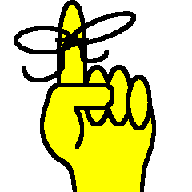
\includegraphics[width=0.7cm]{figures/reminder.pdf}}}}

% Define command to insert gesture image
\newcommand{\gesture}[1]{\marginlabel{{\it#1{\phantom{aa}}}\parbox{1.1cm}{\hspace{-3mm}
\includegraphics[width=0.8cm]{figures/gesture.pdf}}}}
%
% Define command to insert warning image
\newcommand{\warning}[0]{\marginlabel{\parbox{1.3cm}{
\includegraphics[width=0.9cm]{figures/warning.pdf}}}}
%
% Define command to insert Achtung image
\newcommand{\achtung}[0]{\marginlabel{\parbox{1.3cm}{
\includegraphics[width=2.5em]{figures/warning.pdf}}}}
%
% Define command to insert a flash image
\newcommand{\blitz}[0]{\marginlabel{\parbox{1.3cm}{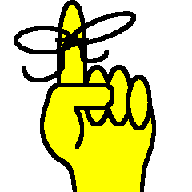
\includegraphics[height=2.0em]{figures/reminder.pdf}}}}
%
% Define command to insert a stop
\newcommand{\halt}[0]{\marginlabel{\parbox{1.3cm}{
\includegraphics[height=2.0em]{figures/warning.pdf}}}}
%
% Define command to reference a configuration item
\newcommand{\config}[1]{\marginlabel{\ref{conf:#1}\parbox{1.3cm}{
\includegraphics[width=0.8cm]{figures/config.pdf}}}}
%
% Potentially overdue ``InfoBox'' style macro but sometimes used... so ..let it be alive ..
\newcommand{\InfoBox}[0]{{InfoBox}}
%
% Define command to put a menu label on the margin
\newcommand{\menulabel}[1]{\marginpar{\parbox{5.0cm}{\raggedright #1}}}
%
% Define command to draw a sketch on the margin
\newcommand{\sketch}[1]{\marginpar{\parbox{4.750cm}{\includegraphics[angle=0,width=0.9\linewidth,keepaspectratio='true']{#1}}}}
%
% Define command to draw a small sketch on the margin
\newcommand{\smallsketch}[1]{\marginpar{\includegraphics[angle=0,keepaspectratio='true']{#1}}}
%
% Enumerated todo's for the todonotes package
\newcounter{todocounter}
\newcommand{\todonum}[2][]{\stepcounter{todocounter}\todo[#1]{\thetodocounter: #2}}
%
% dies nette Makro bringt mir die aktuelle Version der bearbeiteten XCSoar-Verrion aufs Papier 
\newcommand{\version}{\begingroup\catcode`\_=\active\input{VERSION.txt}\endgroup}
%
%Anführungszeichen per Tastatur einfach so eingeben -> "
\shorthandoff{"}%

\def\maketitle{%
  \null
  \thispagestyle{empty}%
  \begin{maxipage}
    \begin{center}
    
\includegraphics[angle=0,width=\textwidth,keepaspectratio='true']{xcsoar-title.png}
    \end{center}
    \begin{center}
      \normalfont\huge\textsf{Glide~Computer and Navigation~System}\par
    \end{center}
    \vskip 1cm
    \begin{center}
      \normalfont\huge\textsf{\@title}\par
    \end{center}
    \vskip 1cm
  \end{maxipage}

  \vfill

  \begin{flushright}
    \large \strut {
      \sf
      \begin{tabular}{r}
      Manual version 1.6 \\
      \today \\
      For XCSoar version 6.0 \\
      \xcsoarwebsite \\
      \end{tabular} 
    } 
    \par
  \end{flushright}
  \par
  \vfil
  \vfil
  \null
  \cleardoublepage
}

\usepackage{setspace}
\newcommand{\InfoBox}[0]{{InfoBox}}
\begin{document}
\maketitle

\begingroup
\setlength{\parskip}{0.1\baselineskip}
\tableofcontents
\endgroup

%%%%%%%%%%%%%%%%%%%%%%

\chapter*{Preface}

This manual applies to XCSoar version 6.0.  The authors reserve the
right to update this manual as enhancements are made throughout the
life of this product.

\section*{Warnings and precautions}

\warning IT IS THE USER'S RESPONSIBILITY TO USE THIS SOFTWARE PRUDENTLY. THIS
SOFTWARE IS INTENDED TO BE USED ONLY AS A NAVIGATION AID AND MUST NOT
BE USED FOR ANY PURPOSE REQUIRING PRECISE MEASUREMENT OF DIRECTION,
DISTANCE, LOCATION, OR TOPOGRAPHY. THIS SOFTWARE SHOULD NOT BE USED AS
AN AID TO DETERMINE GROUND PROXIMITY FOR AIRCRAFT NAVIGATION.
THIS SOFTWARE SHOULD NOT BE USED AS A TRAFFIC COLLISION AVOIDANCE SYSTEM.


\section*{Legal notices}

\subsection*{Software license agreement}

This software is released according to the GNU General Public License
Version~2.  See Appendix~\ref{cha:gnu-general-public} for the full
text of the agreement and warranty notice.

\subsection*{Limited liability}

In no event shall XCSoar, or its principals, shareholders, officers,
employees, affiliates, contractors, subsidiaries, or parent
organizations, be liable for any incidental, consequential, or
punitive damages whatsoever relating to the use of the Product.

\subsection*{Disclaimer}

This product, and all accompanying files, data and materials, are
distributed "as is" and with no warranties of any kind, whether
express or implied.  This product is used entirely at the risk of the
user.  Although great care has been taken to eliminate defects during
its development it is not claimed to be fault-free. No claims are made
regarding its correctness, reliability or fitness for any particular
purpose.  The XCSoar project developers and contributors shall not be
liable for errors contained herein or for incidental or consequential
damages, loss of data or personal injury in connection with
furnishing, performance, or use of this material.


%%%%%%%%%%%%%%%%%%%%%%%%%%%%%%%%%%%%%%%%%%%%%%%%%%%%%%%%%%%%%%%%
\chapter{Introduction}\label{cha:introduction}
This document is a pilot's manual for XCSoar, an open source glide
navigation system for Pocket PC devices.  The audience is assumed to
have a sound knowledge of the fundamental theory of flight for
gliders, and at least a basic working knowledge of cross-country soaring.

Updates to the XCSoar software may result in some of this manual being
out of date.  You should read the release notes distributed with the
software to keep track of changes.  Updates to the manual and software
are available from 
\begin{quote}
\xcsoarwebsite
\end{quote}

\section{Organisation of this manual}

This manual is broadly organised into the major functions of the
software from a pilot's perspective.  The remainder of this chapter
deals with how to download, install and run the software on various
platforms.  Chapter~\ref{cha:interface} introduces the user interface
concepts and gives an overview of the display.

Chapter~\ref{cha:navigation} describes the moving map part of the
display in greater detail and describes how the software can assist in
general navigation.  Chapter~\ref{cha:tasks} describes how
cross-country tasks are specified and flown, and presents some of the
analysis tools available to pilots to help improve their performance.
Chapter~\ref{cha:glide} goes into further detail on the glide computer
functions as it is important for pilots to be aware of how the
computer performs its calculations.

Chapter~\ref{cha:atmosph} describes how the computer can interface to
variometers and other air data sensors, and how it uses these
measurements to provide various models of the atmosphere, in
particular on winds and thermal convection.
Chapter~\ref{cha:airspace} describes how XCSoar can assist in managing
flight in special use airspace and the FLARM collision awareness
system.  Chapter~\ref{cha:avionics-airframe} deals with systems
integration and systems diagnostics, the integration of XCSoar with
communications devices and with airframe switches.

The remainder of the manual contains mainly reference material.
Chapter~\ref{cha:infobox} lists the types of information that can be
displayed in the grid of InfoBoxes next to the map display.  The
configuration of the software is described in detail in
Chapter~\ref{cha:configuration}.  The formats of the various data
files that program uses, as well as where to obtain them from and how
to edit them, is described in Chapter~\ref{cha:data-files}.

Finally, a short history and discussion of XCSoar's development
process is presented in Chapter~\ref{cha:history-development}.

\section{Notes}

\subsection*{Terminology}
A variety of terms may be used to describe Pocket PC devices,
including `organiser' and Portable Digital Assistant (PDA).  XCSoar is
available on triadis Engineering's Altair glide computer, which is
formally an Electronic Flight Instrumentation System.  Throughout this
document, these terms are used interchangeably to refer to whatever
hardware XCSoar is running on.

\subsection*{Screen shots}

Throughout this manual are several screen-shots of XCSoar.  These are
taken from the program running on a variety of hardware platforms.
Each platform may have different screen resolutions, layouts and
fonts, and so there may be slight differences in the appearance of the
display.  Most of the screen-shots in this manual are of XCSoar running
in landscape orientation.

\section{System requirements}
\begin{description}
\item[PC or laptop]
Running Microsoft ActiveSync, to enable installation to a Pocket PC
device.  The PC is used for XCSoar installation on Pocket PC devices,
and is used for the PC version of XCSoar.  Refer to the XCSoar website
for installation instructions when using Linux or MacOS operating
systems.
\item[Pocket PC]
Microsoft Windows CE Version 3.0 or later (PocketPC), MIPS and ARM
processors.  Refer to the XCSoar website for a list of devices verified
to work correctly.  Devices with Symbian, Palm OS or Linux operating
systems are not currently supported.
%Section~\ref{sec:pocket-pc-devices} lists several suitable Pocket PC
%devices.
\item[GPS data source]
NMEA-0183 data source that outputs GPRMC and GPGGA sentences.
Suitable devices include handheld serial GPS devices, glider flight
loggers, bluetooth GPS devices, GPS-integrated variometers, and FLARM.
%Section~\ref{sec:gps-devices} lists several suitable GPS data sources.
Many flight simulators can output NMEA data and so can be used with
XCSoar.  Some Pocket PC devices now have an internal GPS.
Up to two GPS devices may be used simultaneously, giving XCSoar 
a degree of redundancy of the GPS fixes. 
\item[Altair]
The Altair glide computer by triadis Engineering is a glide computer
factory installed with XCSoar.  The Altair PRO version also contains
an internal GPS.
\end{description}

\section{Downloading XCSoar}
The software is available as a free download from the XCSoar website~\xcsoarwebsite.  Follow the links to the download section.

Several versions are available for different operating systems:
\begin{description}
\item[Pocket PC] This version is used by Pocket PC (Windows Mobile) organisers.
\item[Altair] This version is used by the Altair glide computer.
\item[PC]  This version is used on Windows personal computers.
\end{description}

\subsection*{Pocket PC Installer}
Download the relevant package for your Pocket PC operating system
version and save it to disk:
\begin{description}
\item[PPC2000] For Pocket PC 2002 and older, MIPS or ARM CPU.
\item[PPC2003] For Pocket PC 2003, Pocket PC 2003 Second Edition, 
  and Windows Mobile 5.0 and Windows Mobile 6.0.
\item[ALL] This package contains the executable programs for all
 operating systems versions listed above.
\end{description}

\begin{center}
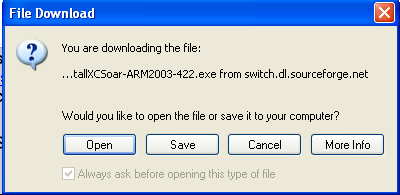
\includegraphics[angle=0,width=\linewidth,keepaspectratio='true']{figures/XCS_Download.png}
\end{center}

%XXX SmartPhone?

\subsection*{Additional files}

Additional data files, such as terrain and topology, special use
airspace, waypoints etc.\ can also be downloaded.  The files used by
XCSoar are described in Chapter~\ref{cha:data-files}.

All data files should be copied into the directory
\texttt{XCSoarData}.  The location of this directory is determined
with the following method:

\begin{itemize}
\item on PC, it is always in your personal folder (``\texttt{My
  Documents}'')
\item if you start XCSoar from a SD card, it is always in the root of
  that SD card (e.g. ``\texttt{/SD Card/XCSoarData}'')
\item if \texttt{XCSoarData} already exists on any SD card inserted
  during XCSoar startup, this one is used
\item if none of the above applies, then it is in your personal folder
  (``\texttt{/My Documents}'')
\end{itemize}

It is recommended to create \texttt{XCSoarData} on a SD card, because
you can easily update the data files on your PC.


\section{Installation}
\subsection*{Installation of Pocket PC version from Windows PC}

Prior to performing any installation, it is a good idea to backup your
organiser for extra safety.

The following sequence describes how to install XCSoar from Windows:
\begin{enumerate}
\item Place your PocketPC in its cradle and make sure
 you have MS ActiveSync running.
\begin{center}
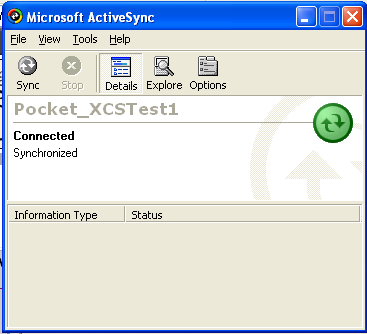
\includegraphics[angle=0,width=\linewidth,keepaspectratio='true']{figures/XCS_ActiveSync.png}
\end{center}

\item Run the installation program \verb|Install-XCSoar-XXX-YYY.exe| 
  (where XXX and YYY refer to the version number and operating system
  version respectively).

\begin{center}
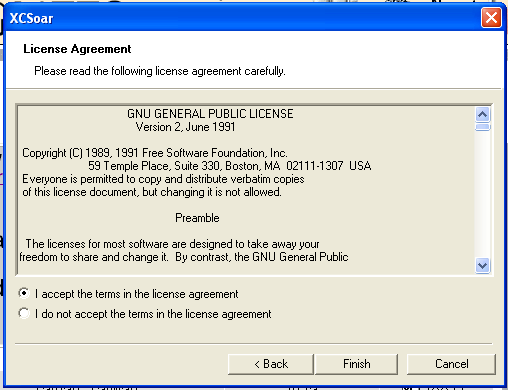
\includegraphics[angle=0,width=\linewidth,keepaspectratio='true']{figures/XCS_License.png}
\end{center}

\item Read and accept the license
\item Follow the prompts in the installation program and also follow the prompts on the organiser.

\begin{center}
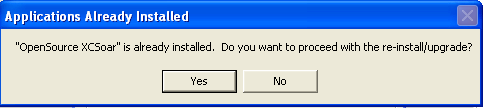
\includegraphics[angle=0,width=\linewidth,keepaspectratio='true']{figures/XCS_Windows.png}
\end{center}

\item XCSoar is now installed.
\item Perform a reset of your device.  See the operating instructions for your
  organiser about how to do this.
\item After the reset, the XCSoar `FLY' and `SIM' launcher icons will
 be visible on the Today screen.

\begin{center}
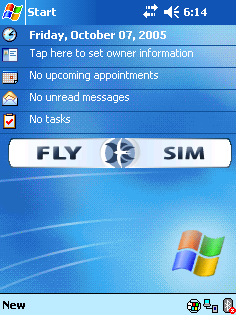
\includegraphics[angle=0,width=0.6\linewidth,keepaspectratio='true']{figures/XCS_Today.png}
\end{center}

\end{enumerate}

It is a good idea to assign one of your PocketPC hardware buttons to
run XCSoar. See your PocketPC manual for details of how to do this.

Owners of Compaq Aero PocketPCs may find it useful to enable `Game
Keys'.

\subsection*{Installation of Pocket PC version from a Pocket PC CAB file}

You can download the CAB file appropriate for your organiser and
install it onto a nonvolatile storage card like a Compact Flash or
Secure Digital card. Place it in your organiser. Use the File Manager
on your organiser to find the CAB and click on it to execute
it. Follow the onscreen instructions, the CAB file will be deleted
after installation.

Alternatively you can download the CAB file from sourceforge through
your Internet Explorer on your organiser and install it that way.

\tip It is generally a good idea to keep the CAB file on the storage card
so that if the organiser's power fails and the memory is lost, XCSoar
can be reinstalled.

\subsection*{Installation of PC version}

The file \verb|XCSoarPC.zip| needs to be unzipped using a utility
program such as WinZip.

Development of a proper windows installer for the PC version is in
progress.  For now, any additional data files used by the PC version
must be placed in the \verb|My Documents\XCSoarData| directory.

\section{Running XCSoar}
%\subsection*{Fly and simulator modes}

Two versions of XCSoar are available, FLY and SIM. 
\begin{description}
\item[FLY] This mode is used when actually flying.  The simulator is 
  disabled and serial communications are active. 
\item[SIM] This starts XCSoar in simulator mode, no serial communications
  are attempted.
\end{description}

The simulator contains a simple interface allowing the user to fly
the glider about.  Dragging the map screen (with touchscreen or
mouse) causes the glider to move in the direction of the drag, the
speed being proportional to the length of the drag.  In SIM mode, the
aircraft altitude can be adjusted by selecting the GPS altitude
{\InfoBox} (marked \infobox{H GPS}), and pressing the up or down keys.

\tip It is recommended that on Pocket PC devices, no other programs
 are running while XCSoar is used in flights.  This gives the best
 possible performance and responsiveness of the program.

\subsection*{XCSoar Pocket PC version}
The program can be run in either of two modes by pressing the `FLY' or
`SIM' launcher on the Today screen.

In addition to starting the program through the use of the launcher,
it is also possible to use the File Explorer to locate the
\verb|XCSoar.exe| or \verb|XCSoarSimulator.exe| programs 
(respectively FLY and SIM modes).  Typically these are located in the
\verb|Program Files\XCSoar| directory.

\subsection*{Altair version}
XCSoar starts up automatically when Altair is powered on.
The PWR/ESC button (top left) has multiple functions:
\begin{description}
\item[Powering on]  Press and hold the PWR/ESC button for one second.
  The LED in the button will light up, and XCSoar will start after
  Altair has booted.
\item[Powering off]  Press and hold the PWR/ESC button for 3 seconds.
  Altair will switch off.
\item[Escape] Pressing the PWR/ESC button quickly acts as an
Escape key, typically used to close dialog pages or as a cancel function.
\end{description}

The Altair version of XCSoar does not include a simulator mode.

\subsection*{XCSoar PC version}
The program can be run by opening the explorer window, find the
\verb|C:\XCSoar| directory, and double clicking on the program file:
\begin{description}
\item[FLY] Run XCSoarPC.exe 
\item[SIM] Run XCSoarPCSim.exe
\end{description}

The program command line options allows the screen orientation of
the display to be defined:
\begin{description}
\item[-portrait] The screen is 480 pixels wide, 640 pixels high.
\item[-square] The screen is 480 pixels wide, 480 pixels high.
\item[-landscape] The screen is 640 pixels wide, 480 pixels high.
\item[-small] Draws the screen at half size.  This is useful for using XCSoar in
 conjunction with flight simulators e.g.\ Condor.
\end{description}
To change the default screen orientation, it is convenient to create a
shortcut to the program, then right click on the shortcut icon, then
click ``Shortcut''.  In the field ``Target'' add the desired option
listed above.

\subsection*{Start-up and user profiles}

When XCSoar starts up, it displays a small window with a safety
reminder.  To proceed, press Enter (to acknowledge the reminder).
There is also a data field that allows the user to select a profile
from a list.  This allows multiple independent configurations of
XCSoar to coexist for different purposes, such as:
\begin{itemize}
\item Different pilots
\item Competition versus casual flying
\item Flying in different locations
\end{itemize}

\begin{center}
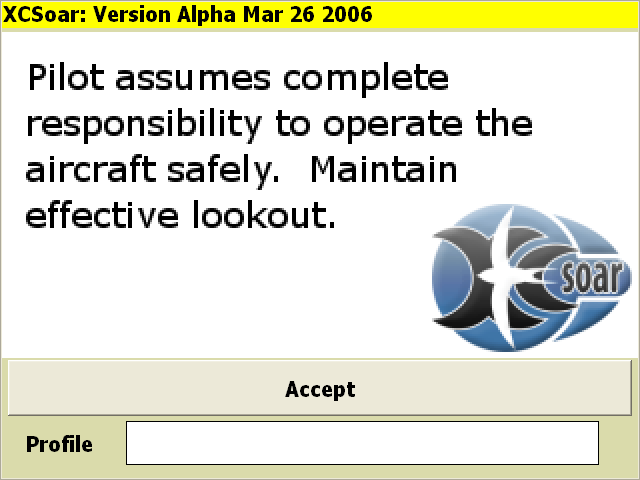
\includegraphics[angle=0,width=0.7\linewidth,keepaspectratio='true']{figures/disclaimer.png}
\end{center}

This customisation of profiles is described briefly in
Chapter~\ref{cha:data-files} and in greater detail in the {\em XCSoar
Advanced Configuration Manual}.  When multiple profiles are available,
changes to configuration settings will only affect the profile
selected at start-up; others are unaffected.

\subsection*{Splash screen}

When XCSoar starts up, shuts down, or loads large files, such as
airspace, waypoints etc, a splash screen is presented while the file
is being loaded.  This screen has a progress bar which indicates the
file loading activity, and a short line of text describing the action
that is being performed.

This screen also displays the software version information.

\subsection*{Last flight statistics}

The previous flight's statistics are saved when XCSoar exits, and
loaded at startup.  This allows the flight to be reviewed after
shutting down Altair.  Statistics are reset on takeoff so they will
not affect the next flight.  Note that these persistent flight
statistics use approximately 85 kilobytes of storage.

\subsection*{Persistent settings}

The basic settings (MacCready setting, Bugs, Ballast, QNH, maximum
forecast temperature) are preserved when XCSoar shuts down and
restored when XCSoar initialises.  

\subsection*{Exiting the program}

For PDA and PC versions, XCSoar is shut down from the menu:
\begin{quote}
\bmenu{INFO}\blink\bmenu{INFO}\blink\bmenu{INFO}\blink\bmenu{Exit}
\end{quote}

For PC versions, XCSoar can also be shut down by clicking the close icon
on the XCSoar window.

For Altair, XCSoar is shut down by holding the PWR button for two seconds or
more.


\section{Through-life support}

\subsection*{Troubleshooting}

A small team of dedicated developers produces XCSoar.  Although we are
happy to help with the use of our software, we cannot teach you about
basics of modern information technology. There are ample existing
resources dealing with these.  If you have a question about XCSoar
please email us at 
\begin{quote}
\url{xcsoar-user@lists.sourceforge.net}.
\end{quote}

Any frequent questions will be added to this document and to the Frequently
Asked Questions (FAQ) section of the XCSoar website.

You may also find it useful to subscribe to the XCSoar users mailing
list so you will be kept up to date with latest developments.

A log file of the startup functions of XCSoar is generated to the file
\verb|xcsoar-startup.log|.  This can be sent to the XCSoar developers
to help determine the cause if the program crashes at startup.

For Altair users, the startup file is transferred to the `FromAltair'
directory by AltairSync if a USB drive is plugged in when Altair is
first switched on.

\subsection*{Updates}

You should periodically visit the XCSoar website to check for program
updates.  The installation procedure described above can typically be
repeated in order to upgrade the software.  All user configuration
settings and data files will be preserved during the
re-installation/upgrade.

It is also recommended to periodically check for updates to data
files, particularly Special Use Airspace, which may be subject to
change by the national civil aviation authority.

Like any complex software program, XCSoar may be subject to software
bugs, so if you find any, please report them to the XCSoar developers
by using the bug tracker at 
\begin{quote}
\url{http://sourceforge.net/projects/xcsoar}
\end{quote}
or email
\begin{quote}
\url{xcsoar-devel@lists.sourceforge.net}
\end{quote} 

\subsection*{Updating XCSoar on Altair}

Updating XCSoar on Altair involves downloading the latest program file
{\tt XCSoarAltair-YYY-CRCXX.exe}, copying it to a USB memory stick,
then using the AltairSync utility on the Altair device to complete the
installation.  Refer to the {\em Altair Owner's Manual} for details.

Other data and program files can be transferred to Altair in a similar
way.

\section{Training}

For safety of self and others, pilots using XCSoar are advised to
train with it on the ground and become familiar with its interface and
features prior to flight.

\subsection*{Using XCSoarPC}

The XCSoarPC simulator may be used to become familiar with XCSoar's
interface and functionality in the comfort of one's home.  All files
and configuration used by XCSoarPC are identical to the Pocket PC or
Altair versions, so it can be helpful to try out customisations on the
PC version before using them in flight.

The XCSoarPC fly version can also be connected to external devices
and operates just as the Pocket PC FLY and Altair versions do.
Suggested uses include:
\begin{itemize}
\item Connect the PC to a FLARM device to use XCSoarPC as a ground
station display of FLARM-equipped traffic.
\item Connect the PC to an intelligent variometer such as Vega to
test configuration settings of the variometer.
\end{itemize}

\subsection*{Using XCSoar with a flight simulator}

A good way to learn how to use XCSoar is to connect the Pocket PC
device to a PC running a flight simulator that can output NMEA
sentences to the serial port.  Suitable simulators include Condor and
X-Plane.  

The benefit of this form of training is that XCSoar can be used in FLY
mode, so it behaves exactly as if you were really flying, and you can
get a good feel for how the program works while you are flying the
simulator.

\section{Using XCSoar safely}

The use of an interactive system like XCSoar in flight carries with it
certain risks due to the potential distraction of the pilot from
maintaining situational awareness and eyes outside the cockpit.

The philosophy guiding the design and development of the software is
to try to reduce this distraction by minimising the need for user
interactions as much as possible, and by presenting information in a
clear fashion able to be interpreted in a glance.

Pilots using XCSoar must take responsibility for using the system safely.
Good practice in the use of XCSoar includes:
\begin{itemize}
\item Becoming familiar with the system thoroughly through training on 
  the ground.
\item Performing clearing turns before interacting with XCSoar in flight
  in order to ensure there is no collision risk with other traffic.
\item Setting up the system to take advantage of automatic functions
  and input events so that user interactions can be minimised.  If you
  find yourself mechanically performing certain interactions frequently,
  ask yourself (or other XCSoar users) if the software can be made to do 
  these interactions for you.
\end{itemize}

%%%%%%%%%%%%%%%%%%%%%%%%%%%%%%%%%%%%%%%%%%%%%%%%%%%%%%%%%%%%%%%%%%%%%
\chapter{User Interface}\label{cha:interface}
This chapter describes the fundamental user interface concepts used by
XCSoar, and is intended as an overview.  More detailed descriptions
are given in following chapters.

\begin{center}
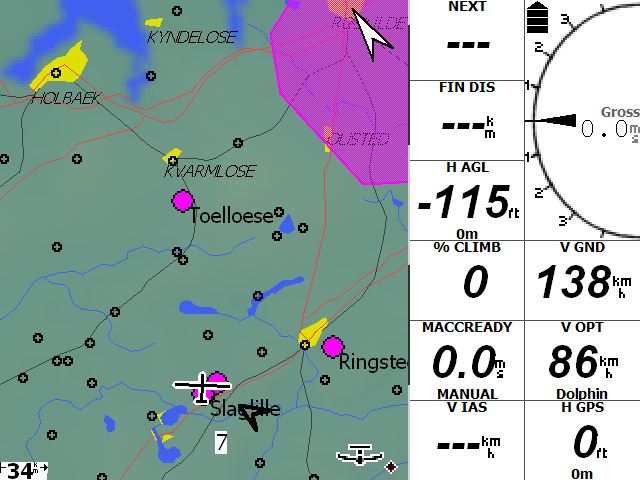
\includegraphics[angle=0,width=\linewidth,keepaspectratio='true']{figures/plain.png}
\end{center}

The XCSoar display is composed of several parts:
\begin{description}
\item[Map area] The bulk of the screen is dedicated to the GPS moving 
 map display.  Various symbols relating to glide computer information
 are overlaid on the map area.  Icons and text may appear along the
 lower edge of the screen to indicate status of connected devices,
 operating modes etc.
\item[{\InfoBox}es] A grid of data values is displayed either along
  the top and bottom of the screen (portrait display) or to the right
  of the screen (landscape display).  These so-called {\InfoBox}es
  display data from the GPS and other input devices as well as data
  generated by the glide computer.
\item[Gauges]  Gauges provide instrumentation displays.
All gauges are optional and some may only have meaningful information
displayed when XCSoar is connected to a supported instrument.
\item[Button labels and menus] Hardware buttons on the Pocket PC
  can be used to bring up and navigate smaller onscreen menus that
  are typically laid out such that menu items can be selected by pressing
  the button adjacent to the item.  If the Pocket PC has a touch screen,
  then menu items can be selected by touching them.  These buttons
  are drawn in black text on a green background.
\item[Status messages]  Text is displayed over the map area in status
 message boxes.  This text is used to present detailed information to
 the pilot when certain events occur. 
\item[Dialog windows] Larger dialog windows, usually containing
  graphics and buttons, are used to present detailed data to the pilot
  regarding waypoint details, statistics and analysis etc. 
\item[Main menu] The main menu is accessible by double clicking the
  map area to bring up a ``Menu'' button, which if touched brings up a
  full-page dialog containing the main menu items.  If the Menu button
  is not pressed again after more than 10 seconds; it disappears again
  so as to not obscure the map area.  This button is not available for
  non-touchscreen computers (such as Altair).
\end{description}

There are several ways to interact with XCSoar:
\begin{itemize}
\item Touching certain map elements
\item Touching InfoBoxes and onscreen menu buttons
\item `Dragging' the screen (touching the screen and moving before releasing)
\item Pressing application buttons on the Pocket PC device.
\item Pressing the cursor keys on the Pocket PC device.
\item Pressing keys or switches on an instrument connected to XCSoar.
\end{itemize}
Depending on the particular hardware used with XCSoar, not all of
these methods of interaction are possible, and there may be different
numbers or assignments of buttons.  
%Refer to
%Chapter~\ref{cha:hardware} for details of major hardware
%configurations.  

For the PC version of XCSoar, clicking the mouse over an item is
equivalent to touching it.

Altair does not have a touch screen; all user interaction is performed
via physical buttons, switches or other external interface devices if
connected.

\section{Button labels and menus}
The button menu is a set of buttons drawn on the screen and activated
by touch or hardware button presses.  Using buttons and the button
menu are the primary ways the user interacts with XCSoar.  

\begin{center}
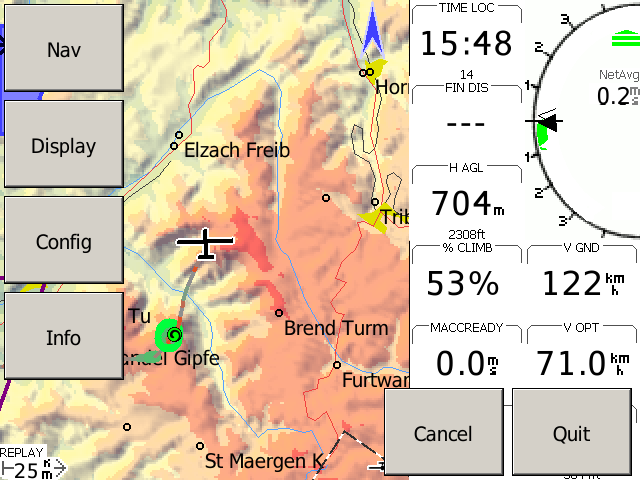
\includegraphics[angle=0,width=\linewidth,keepaspectratio='true']{figures/buttonmenu.png}
\end{center}

\subsection*{Interface basics}

The menu is organised into different groups of functions, usually in
the form of a hierarchy.  The specific menu layout depends on the
hardware button configurations and computer platform, and may also be
customised by the user as described in the {\em XCSoar Advanced
Configuration Manual}.

XCSoar can also accept input from external keyboards, game-pads,
joysticks, stick grip switches etc.  A wide variety of functions can
be assigned to these inputs.

For Altair, there are four major menus, activated by pressing one of
the vertical strip of hardware buttons on the left of the display.
When a menu is activated, a strip of onscreen buttons appear along the
bottom of the display.  Pressing the particular menu button again will
cycle through several pages of items.  Pressing the corresponding
horizontal button will activate that item.  At the last page, pressing
the menu button again will turn that menu off and the horizontal strip
of onscreen buttons disappear.  

On the PC version (XCSoarPC), these mode buttons are activated by the
1,2,3,4 keys.  The 6,7,8,9,0 keys correspond to the horizontal strip
of buttons.

On the PDA version, the mode buttons are activated by the keys to the
side of the joystick/rocker button.

By convention, buttons labeled with a trailing slash,
e.g.~\bmenu{NAV/} means that pressing the button will show more items.
Buttons labeled with a leading slash, e.g.~\bmenu{/NAV} means that
pressing the button will close that menu.

If the user doesn't interact with the computer for a long time, the
menu will close automatically.  This menu timeout is configurable.
The escape key on PC, or the PWR/ESC button on Altair, can
also be used to close the current menu.

Menu button labels appear as grey text instead of black if the
corresponding function is not available.  For example, the ``Waypoint
lookup'' function will appear grey if there are no waypoints loaded.

Several menu button labels have dynamic text based on context, in
order to make it clearer as to what happens when the button is
pressed.  The convention is used that a button's label describes what
will happen when the button is pressed.  For example, if the button
says \button{Auto Mc ON}, then pressing the button will turn auto
MacCready on, and the button label will then change to \button{Auto Mc
Off}.  In the menu list described below, generic labels are used.

\subsection*{Menu overview}
This section describes the default layout of the menu system on all
platforms.  The functions performed by each button are explained more
fully in following chapters.

The primary menu buttons are activated by each of the vertical strip of buttons on Altair, from top to bottom:
\begin{jspecs}
\item[\bmenu{NAV}] Actions for navigation control, primarily cross-country gliding tasks.
\item[\bmenu{DISPLAY}] Actions to control the display
\item[\bmenu{CONFIG}] Configuration of XCSoar, connected devices, and in-flight settings
\item[\bmenu{INFO}] Activates various informational dialog windows.
\end{jspecs}

For the PC version, the keys 1, 2, 3, and 4 activate the NAV, DISPLAY,
CONFIG, and INFO menus.

\subsection*{NAV menu}

\jindent{\bmenut{Task}{Calc}}{  Displays the task calculator dialog 
}
\jindent{\bmenut{Arm}{Advance}}{ Arms the automatic task waypoint trigger
}
\jindent{\bmenut{Waypoint}{Previous}}{ Selects the previous waypoint in the task
}
\jindent{\bmenut{Waypoint}{Next}}{ Selects the next waypoint in the task
}
\jindent{\bmenut{Waypoint}{Lookup}}{  Displays the waypoint selector dialog
}
\jindent{\bmenut{Task}{Edit}}{ Displays the task editor
}
\jindent{\bmenut{Task}{Save}}{ Saves the current task to the default, so when restarting
  XCSoar, the task is restored.
}
\jindent{\bmenut{Task}{Abort}}{ Aborts/resumes the current task.
}
\jindent{\bmenut{Force}{Final}}{ Toggles between automatic and forced final
 glide mode.
}
\jindent{\bmenut{Team}{code}}{ Displays the team code dialog.
}

\subsection*{DISPLAY menu}
\jindent{\bmenus{Pan}}{  Activates pan map mode
}
\jindent{\bmenut{Zoom}{In}}{ Zooms in the map display
}
\jindent{\bmenut{Zoom}{Out}}{ Zooms out the map display
}
\jindent{\bmenut{Mark}{Drop}}{ Drops a marker at the current glider location
}
\jindent{\bmenut{Full}{Screen}}{ Switches between full screen and normal display
}
\jindent{\bmenut{Zoom}{Auto}}{ Toggles automatic zooming
}
\jindent{\bmenut{Snail}{Trail}}{ Toggles display of snail trail
}
\jindent{\bmenut{Terrain}{Toggle}}{ Toggles display of terrain and topology
}
\jindent{\bmenus{Bright}}{ Adjusts screen brightness
}
\jindent{\bmenut{Declutter}{Labels}}{ Toggles display of topology and non-task labels
}

\subsection*{CONFIG menu}
\jindent{\bmenut{MacCready}{$+$}}{ Increases MacCready value
}
\jindent{\bmenut{MacCready}{$-$}}{ Decreases MacCready value
}
\jindent{\bmenut{MacCready}{Auto}}{ Toggles automatic MacCready when in final glide.
}
\jindent{\bmenut{Setup}{Basic}}{ Displays the basic settings (bugs/ballast/QNH) dialog
}
\jindent{\bmenus{Wind}}{ Displays the wind settings dialog 
}
\jindent{\bmenus{Vario/}}{  Control of Vega intelligent variometer, this comprises a sub-menu.
}
\jindent{\bmenut{Setup}{System}}{ Displays the XCSoar configuration dialog 
}
\jindent{\bmenut{Settings}{Airspace}}{  Displays the airspace filter dialog 
}
\jindent{\bmenut{Logger}{Record}}{ Turns on/off XCSoar's software IGC flight
  recorder
}
\jindent{\bmenut{Logger}{Replay}}{ Displays the IGC logger replay remote control dialog
}

\subsection*{INFO menu}
\jindent{\bmenut{Waypoint}{Details}}{ Displays the waypoint details dialog of the 
  active task waypoint 
}
\jindent{\bmenut{Nearest}{Waypoint}}{ Displays the waypoint details dialog of the
  waypoint nearest to the aircraft.
}
\jindent{\bmenut{Nearest}{Airspace}}{
  Displays details of the airspace nearest to the aircraft.
}
\jindent{\bmenut{Check}{List}}{
  Displays the check list dialog.
}
\jindent{\bmenus{Analysis}}{
  Displays the analysis/statistics dialog.
}
\jindent{\bmenus{Status}}{
  Displays the status dialog.
}
\jindent{\bmenus{Weather}}{
  Displays the weather forecast dialog.
}
\jindent{\bmenus{ }}{
  (Blank, reserved for future use)
}
\jindent{\bmenut{Aux}{Infobox}}{
  Toggles the infobox display between normal (flight-mode specific) or
  auxiliary infobox display.
}
\jindent{\bmenut{Message}{Repeat}}{
  Repeats the last status message.
}
\jindent{\bmenus{Exit}}{
  Exits from XCSoar after asking for confirmation.
}

\subsection*{VARIO sub-menu}
The functions in this sub-menu require the Vega intelligent
variometer.  

\jindent{\bmenut{Airframe}{Switches}}{ Displays airframe switch values
}
\jindent{\bmenut{Setup}{Audio}}{ Adjusts volume of sounds 
  produced by XCSoar as well as certain speech announcements 
  by the Vega intelligent variometer.
}
\jindent{\bmenut{Manual}{Demo}}{ Activates Vega variometer manual tone demo
}
\jindent{\bmenut{Setup}{Stall}}{ Opens Vega stall monitor setup dialog
}
\jindent{\bmenut{Vario}{Test/}}{ Test/setup submenu
}
\jindent{\bmenut{ASI}{Zero}}{ Zeros the airspeed indicator.
}
\jindent{\bmenut{Accel}{Zero}}{ Levels/zeros the accelerometers.
}
\jindent{\bmenus{Store}}{ Stores Vega settings to EEPROM
}
\jindent{\bmenut{Cruise}{Demo}}{ Activates Vega variometer cruise tone demo
}
\jindent{\bmenut{Climb}{Demo}}{ Activates Vega variometer climb tone demo
}

\subsection*{Pan mode}

\jindent{\bmenus{Pan}}{  Turns pan mode off
}
\jindent{\bmenut{Zoom}{In}}{ Zooms in the map display
}
\jindent{\bmenut{Zoom}{Out}}{ Zooms out the map display
}
\jindent{\bmenut{Nearest}{Waypoint}}{ Displays the waypoint details dialog of the
  waypoint nearest to the aircraft., or if in pan mode, nearest to the
  cross-hairs at the center of the screen.
}

\subsection*{Default buttons}

When no menu is active, (so-called default mode), the horizontal row
of buttons in Altair perform the following functions (from left to right):

\begin{center}
\begin{tabular}{c c c c c}
 F6 & F7 & F8 & F9 & F0 \\
\bmenut{Setup}{Basic} & \bmenut{Task}{Calc} & \bmenut{Task}{Edit} & \bmenut{Arm}{Advance} & \bmenut{Drop}{mark} \\
\end{tabular}
\end{center}

Pressing ESC on Altair displays labels for these default menu buttons.

For Pocket PC versions in the default mode, the cursor keys perform
the following functions:
\begin{jspecs}
\item[Up key] Zoom in
\item[Down key] Zoom out
\item[Left key] Auto-Zoom toggle
\item[Right key] Pan toggle
\item[Enter] Clear status message or acknowledge airspace warning
\end{jspecs}

For the Altair version in the default mode, the rotary knob performs
the following functions:
\begin{jspecs}
\item[Outer knob counterclockwise] Zoom in
\item[Outer knob clockwise] Zoom out
\item[Inner knob counterclockwise] (No function assigned)
\item[Outer knob clockwise] (No function assigned)
\item[Knob button press] Clear status message or acknowledge airspace warning
\end{jspecs}
In dialog forms, the rotary knob in Altair performs the role of the cursor and
enter keys:
\begin{jspecs}
\item[Outer knob counterclockwise] Up cursor
\item[Outer knob clockwise] Down cursor
\item[Inner knob counterclockwise] Left cursor
\item[Inner knob clockwise] Right cursor
\item[Knob button press] Enter key
\end{jspecs}

For Altair, the buttons along the edge of the display can be used as
alternate ways of navigating in dialogs.  The F4 key (directly above
the rotary knob) can be used as an alternate ENTER key (instead of
pressing the rotary knob) in dialogs.  The F6 and F7 keys (directly to
the right of the rotary knob) can be used to select the next or
previous page in multipage dialogs.

\section{{\InfoBox}es}

The information displayed in the {\InfoBox} fields can be selected from a
wide variety of options (listed in Chapter~\ref{cha:infobox}).  These
fields are also used to set user configurable variables, for example
the MacCready setting.

The specific number and layout of the {\InfoBox} grid depends on the
screen orientation and the device's display size.  For a 320x240 display
Pocket PC in portrait mode, there are four {\InfoBox}es above and four
{\InfoBox}es below the map display.  For landscape mode, there are 9
InfoBoxes to the right of the map display.

\begin{center}

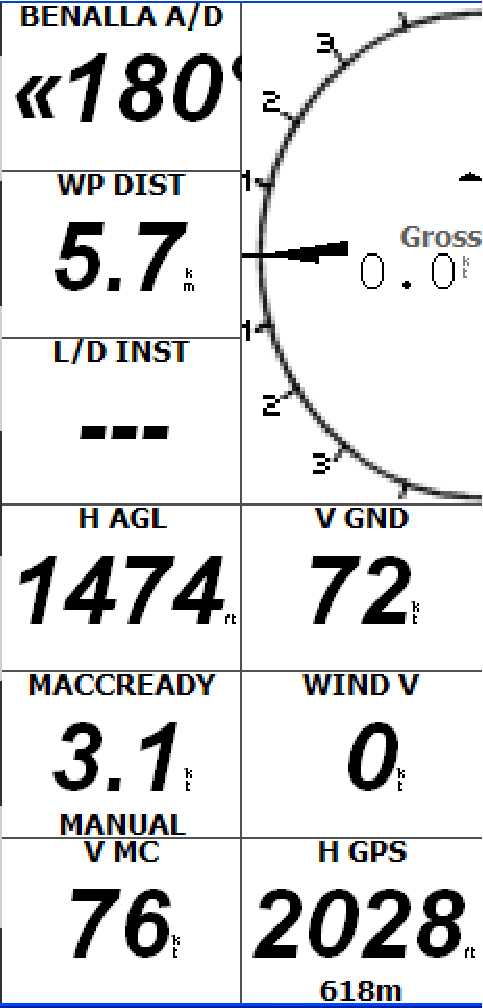
\includegraphics[angle=0,width=0.35\linewidth,keepaspectratio='true']{figures/infoboxes.pdf}

\end{center}

\subsection*{Dynamic menu labels}

Certain menu items now have dynamic labels to make it clearer what
happens when the menu item is selected.  Furthermore, items that are
not available are greyed out to indicate that selecting the menu item
will not do anything.

The convention used for dynamic menu labels is for the labels to
display the action that will be performed once the menu item is
selected.  For example ``Lights ON'' will turn the lights on, and the
menu will be updated to display ``Lights OFF'', which would then if
pressed turn the lights off.  This convention is used throughout.

A selection of key dynamic menu items is presented below, organised by the
old static menu item name.  

\begin{description}
\item[Waypoint next]  
  Greyed out if the task is cleared, or if the active turnpoint is the
  finish.  If on the turnpoint prior to the finish, this displays
  ``Waypoint finish''.
\item[Waypoint previous]  
  Greyed out if the task is cleared, or if the active turnpoint is the
  start and there are no multiple start points.  If there are multiple
  start points and the active turnpoint is the start, then this
  displays ``Cycle start'' to allow selection between the various
  start points.  If on the first turnpoint after the start, this
  displays ``Waypoint Start''.
\item[Declutter labels]  
  This now displays ``Labels ON'' or ``Labels OFF''.
\item[Task calculator]  
  Greyed out if the task is cleared or in task abort.
\item[Arm Advance]  
  Greyed out if Auto or Manual advance mode is active.  Displays ``Arm
  start'' when the active turnpoint is the start and the trigger is
  not armed.  Displays ``Arm Cancel'' if the trigger is armed.
  Displays ``Arm turn'' if the active turnpoint is past the start.
\item[Task save]
  Greyed out if in Task Abort.
\item[Task editor]
  Greyed out if in task abort or no waypoint database.
\end{description}

\subsection*{Screen display modes}

The main display can be presented with the map area and InfoBoxes, or
a full-screen map.  The screen mode can be toggled between the following:
\begin{itemize}
\item Small map area, with flight-mode specific {\InfoBox}es
\item Small map area, showing auxiliary {\InfoBox}es.
\item Full-screen map area, with {\InfoBox}es hidden.
\end{itemize}
This is performed by selecting the menu:
\begin{quote}
\bmenu{DISPLAY}\blink\bmenu{Full screen}
\end{quote}

At any time the InfoBoxes may be toggled between auxiliary and normal from
the menu:
\begin{quote}
\bmenu{INFO}\blink\bmenu{Aux infobox}
\end{quote}

When auxiliary {\InfoBox}es are displayed, the word `AUX' appears at the
lower left corner of the map area.

%{\it SMALL DIAGRAMS SHOWING OVERALL LOOK OF EACH DISPLAY MODE (MAYBE
%IN LANDSCAPE AND PORTRAIT)}
%
\subsection*{Modifying {\InfoBox} values}

(This section applies only when the hardware has
a touchscreen or mouse.)

Some {\InfoBox} values can be changed by the user by selecting the
infobox with the touchscreen or mouse.  Examples of InfoBoxes that can
be adjusted include the MacCready ring setting, and the wind speed.
The procedure for adjusting {\InfoBox} values is as follows:
\begin{enumerate}
\item Highlight the item you wish to modify, by touching the {\InfoBox}.
  The box title border will change colour indicating it is selected.
\item Press the up/down/left/right or enter button on the Pocket PC
  to change the value.  Different {\InfoBox}es allow different buttons to
  be used.
\item The value is now changed.
\item After 10 seconds or so have elapsed without further button pressing,
  the {\InfoBox} will be deactivated so there is no risk of accidental 
  adjustment later.
\end{enumerate}
%1. Ensure that the FileLock menu item is checked.
%\subsection{Changing a Data Display Field}
%\input{infobox-editing.tex}

\section{Status messages}
Status messages appear over the map area to present text for a short
period of time.  The message disappears after the time period has
elapsed, and different types of message have different periods.
Additionally, status messages can be made to disappear by
acknowledging the message.  Acknowledgement is achieved by either
pressing the enter key (rotary knob on Altair), touching the status
message (on touchscreen devices), clicking the screen (mouse enabled
devices).

Additional user buttons may be assigned to a status message repeat
function, which brings up the last message again.

Typical status messages include:
\begin{itemize}
\item Airspace queries
\item Airspace warnings
\item User interface events (e.g.\ changing display modes)
\item Glide computer events (e.g.\ takeoff, turning waypoints)
\end{itemize}

%{\it DIAGRAM SHOWING TYPICAL STATUS MESSAGE}

Note that status messages do not appear while a dialog is on screen,
the messages are buffered and displayed as soon as the dialog is
exited.

\tip The duration each type of status message appears is configurable.
The default duration for important messages is 30 seconds, for other
messages the default duration is 1.5 seconds.

\section{Dialog windows}\label{sec:dialog-windows}

XCSoar contains several dialog windows that can be activated to bring
up additional information and are also used for more complex
interactions with the user, such as editing tasks and configuration
settings.

Some dialogs simply display information, and require no user input.
Other dialogs contain data fields that can be modified or buttons that
can be pressed.  

A cursor appears over the active button or data field.  This cursor
appears as a black border around the corners of the button or field.
Pressing the up/down arrow keys (or rotating the outer knob on
Altair), the cursor will cycle through the next or previous items.
For list items and scrollable text, the up/down arrow key moves the
cursor up or down the list or text, and the left/right arrow keys
move the cursor up or down by one page in long lists.

For PDAs and PC versions, list items can be selected by touching the
item (or left-clicking with the mouse).  Once a list item is selected,
another touch (left click) is equivalent to pressing the enter key.

Pressing the right/left arrow keys (or rotating the inner knob
on Altair), the data field value under the cursor can be modified.
Pressing the enter key (or pressing the rotary knob on Altair)
activates the button or makes a selection from a list.

Dialogs are typically started from the button menu.  

Many of the dialog windows have multiple pages of information and are
controlled in a consistent fashion.  Press the \button{$>$} or
\button{$<$} buttons to select the next or previous page of the
dialog, and the \button{Close} button to make the dialog disappear.

The escape key on a PC, or the PWR/ESC button on Altair, can
also be used to close dialogs.

The user must close the dialog to return to the normal map mode.  When
a dialog has been opened, the menu buttons are disabled until the
dialog is closed.

In some dialogs, items that are not relevant or valid (such as AAT
details when flying a non-AAT task) are not displayed.

%%%%%%%%%%%%%%%%%%%%%%%%%%%%%%%%%%%%%%%%%%%%%%%%%%%%%%%%%%%%%%%%%%%%%%%%

A summary of the major dialogs is presented below.
\begin{description}
\item[Basic settings] Used to modify the polar of the glider both
before and during flight, as well as to set the QNH pressure.
\item[Wind]  Used to modify or adjust the estimated wind magnitude and
direction.
\item[Waypoint details] Describes a waypoint in detail
and has navigation functions such as GOTO, Insert.
\item[Waypoint selector] Used to select a waypoint from the waypoint database.
\item[Task editor]  Used to edit and view cross country tasks.
\item[Task calculator] Allows the pilot to see the effect of various
  changes to the task on final performance.
\item[Analysis] Shows several pages of analysis and statistics about the flight.

\item[Status]  The status dialogs give summaries of the situation of the aircraft, system, task, start and times.
\item[Checklist]  A multi-page custom checklist.
\item[Configuration]  Allows XCSoar and certain connected devices to be configured.
\item[Airspace colours and patterns]  Configuration of colours and patterns of airspace used on the map display.
\item[Airspace filter]  Controls enabling and disabling the display and warnings of each airspace class.
\item[Team code] Allows transfer of coordinates between team mates via a 
 code.
\item[Waypoint edit]  Allows editing of waypoints (name, comment, location,
  altitude, flags).
\end{description}

These dialogs are described in later chapters. with the exception of the
checklist, status and text entry dialogs, which are described below.

\subsection*{Checklist dialog}

The checklist dialog can display several pages of user-defined free
text, typically this is used for checklists.  
This is accessed via the menu under 
\begin{quote}
\bmenu{INFO}\blink\bmenu{Check list}
\end{quote}

These checklists may include: daily inspection, preflight, outlanding,
pre-landing, radio procedures, and aircraft rigging and de-rigging
instructions.  Since the checklists may be long, the up/down keys (or
rotary knob on Altair) may be used to scroll through the text.  Clicking
the \button{$<$} and \button{$>$} buttons select the previous/next checklist.

\begin{center}
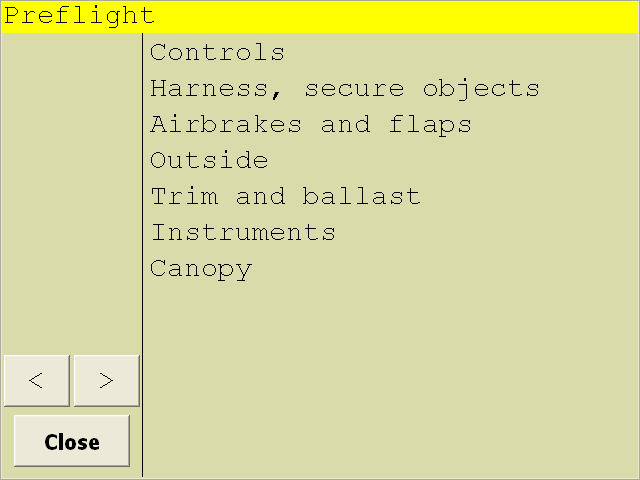
\includegraphics[angle=0,width=\linewidth,keepaspectratio='true']{figures/checklist.png}
\end{center}

\subsection*{Status dialog}

The status dialog is a multipage dialog giving overview information on the 
aircraft, system, task, rules and times.  Clicking
the \button{$<$} and \button{$>$} buttons select the previous/next page.

This is accessed via the menu under 
\begin{quote}
\bmenu{INFO}\blink\bmenu{Status}
\end{quote}

\begin{description}
\item[Aircraft]  Shows the location of the aircraft and nearest waypoint,
  and the maximum height gain.
\begin{center}
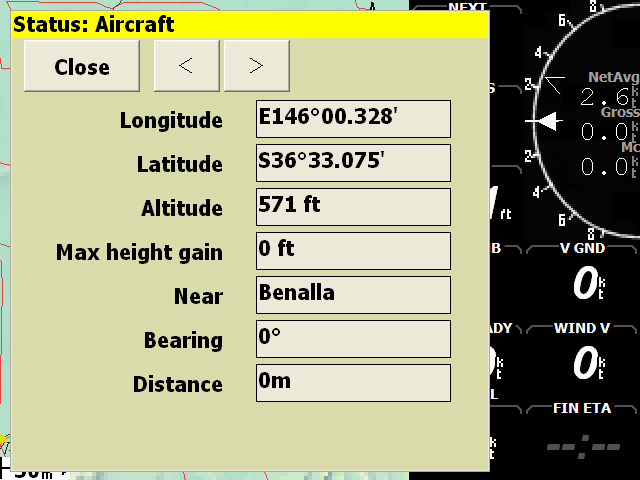
\includegraphics[angle=0,width=\linewidth,keepaspectratio='true']{figures/status-aircraft.png}
\end{center}

\item[System]  Shows the status of connected devices and battery levels

\begin{center}
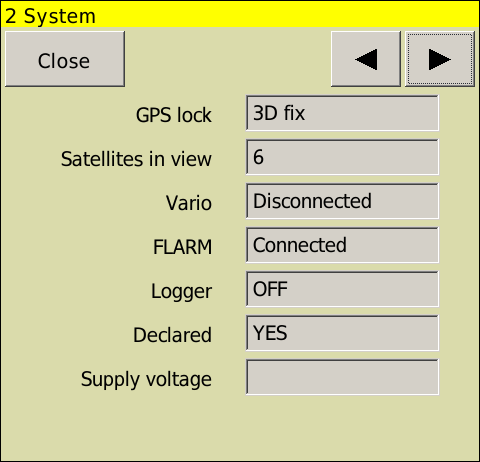
\includegraphics[angle=0,width=\linewidth,keepaspectratio='true']{figures/status-system.png}
\end{center}

\item[Task]  Shows the task speeds, distances achieved and remaining, and AAT
  times.

\begin{center}
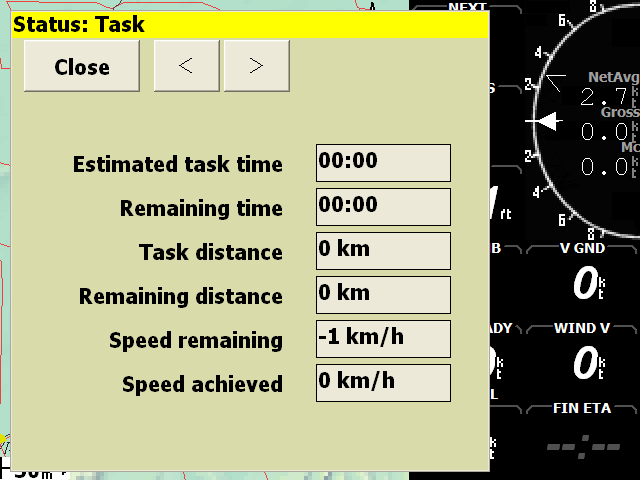
\includegraphics[angle=0,width=\linewidth,keepaspectratio='true']{figures/status-task.png}
\end{center}


\item[Rules]  Shows validity of start/finish according to the rules.

\begin{center}
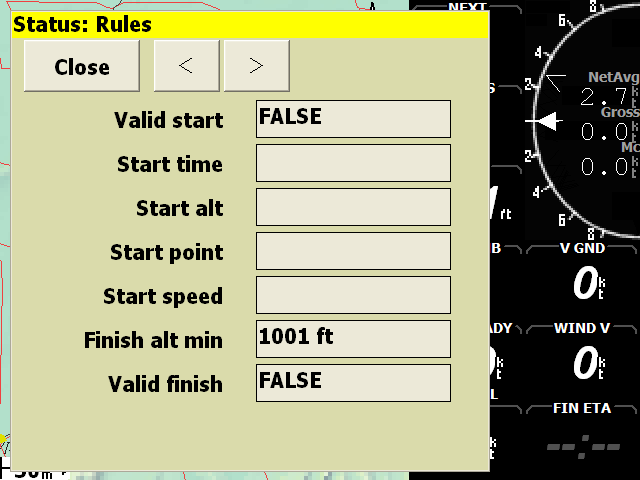
\includegraphics[angle=0,width=\linewidth,keepaspectratio='true']{figures/status-rules.png}
\end{center}

\item[Times]  Shows the local time, flight time, takeoff and landing time,
  and local sunset time.

\begin{center}
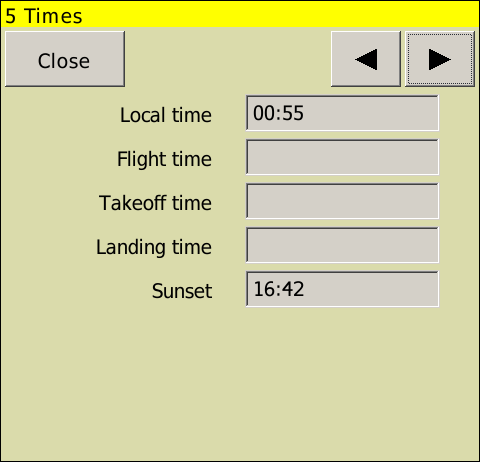
\includegraphics[angle=0,width=\linewidth,keepaspectratio='true']{figures/status-times.png}
\end{center}

\end{description}

\subsection*{Text entry}

A text entry dialog is used for entering text.  This is used for team
code entry, setting file names, waypoint editing, as well as entering
other configuration options, such as pilot name for the logger.

Two ways of entering text are provided. See Section~\ref{sec:status} for details on customisation.

To enter text in HighScore Style, use the A+/A- buttons to adjust the character under the
cursor (underlined character). Clicking the \button{$<$} and \button{$>$} buttons move the
cursor left/right.  

\begin{center}
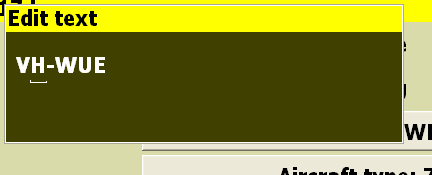
\includegraphics[angle=0,width=\linewidth,keepaspectratio='true']{figures/textentry.png}
\end{center}

To enter text with the touch screen keyboard, press the letters of choice one after the other. In some dialogs (e.g. waypoint editing) only the next letters matching to an entry in the database will be shown. For deleting the last letter use the \button{$<-$} button.

\begin{center}
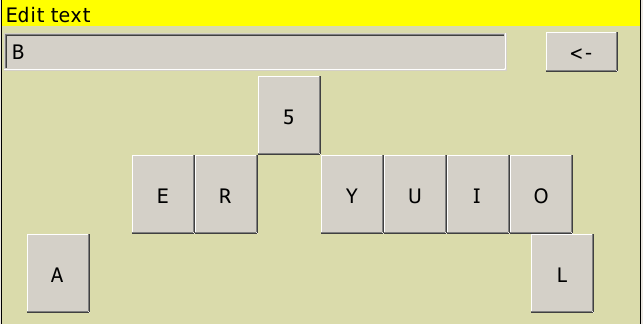
\includegraphics[angle=0,width=\linewidth,keepaspectratio='true']{figures/textentry_keyboard.png}
\end{center}

Press enter or close to exit.

\section{Sounds}

XCSoar generates sounds for different events, and can be configured to
have custom sounds for any event.  See Section~\ref{sec:status} for
details on customisation.

When XCSoar is connected to the Vega intelligent variometer, it sends
commands to Vega's speech system, to give verbal cues and warnings such as:
\begin{itemize}
\item Final glide through terrain
\item Approaching/passing a task waypoint
\item Airspace warnings
\end{itemize}

\section{Screen}

Certain aspects of the look of items on the screen can be adjusted.
The most noticeable of these is whether to display {\InfoBox}es and
gauges in black on white (called inverse colours) or white on black.

For some hardware platforms, the control of the screen hardware 
brightness can be controlled from the brightness dialog
accessible from the menu:
\begin{quote}
\bmenu{DISPLAY}\blink\bmenu{Bright}
\end{quote}

Refer to the {\em Altair User's Manual} for details of the brightness
dialog.

\begin{center}
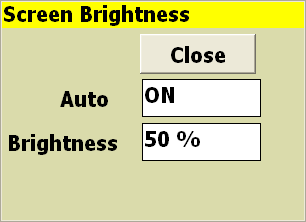
\includegraphics[angle=0,width=0.45\linewidth,keepaspectratio='true']{figures/brightness.png}
\end{center}

\section{Help system}
  A help system now provides descriptive text for properties in
  most dialogs.  When a property is selected, press and hold the
  enter button for two seconds, then release.  A window will open with
  help text describing the property.

\section{Gestures}
  As of version 6.0, XCSoar supports so-called mouse gestures. To activate 
  this feature go to the configuration dialog (Setup System) and enable it.

  To use this feature hold down the mouse button or put the finger on the 
  touchscreen, draw a certain figure and release the mouse 
  button/touchscreen. Depending on the figure that was drawn 
  a certain function is activated. A list of available gestures is 
  shown below. A figure is defined by movements of the 
  cursor in the four directions Up, Down, Left and Right. This means if 
  you hold down the mouse button, drag the mouse to the left 
  and afterwards to the top, the gesture "LU" is detected, which 
  stands for "Left-Up".


  Gestures available on the map screen:
\begin{itemize}
\item U: Equal to pressing the hardware button "Up"
\item D: Equal to pressing the hardware button "Down"
\item L: Equal to pressing the hardware button "Left"
\item R: Equal to pressing the hardware button "Right"
\item DU: Show the menu
\item DR: Show the GoTo dialog
\end{itemize}


  Gestures available on the FLARM radar dialog:
\begin{itemize}
\item U: Zoom in
\item D: Zoom out
\item L: Previous target
\item R: Next target
\item UD: Activate autozoom
\item DR: Open details of selected target
\item RL: Switch additional data show on the side (avg. climb/rel. altitude)
\end{itemize}

%%%%%%%%%%%%%%%%%%%%%%%%%%%%%%%%%%%%%%%%%%%%%%%%%%%%%%%%%%%%%%%%%%%%%
\chapter{Navigation}\label{cha:navigation}
This chapter describes the moving map display as an aid to navigation,
and also describes some of the task and glide related overlays on the
map display.

\section{Map display elements}

\begin{maxipage}
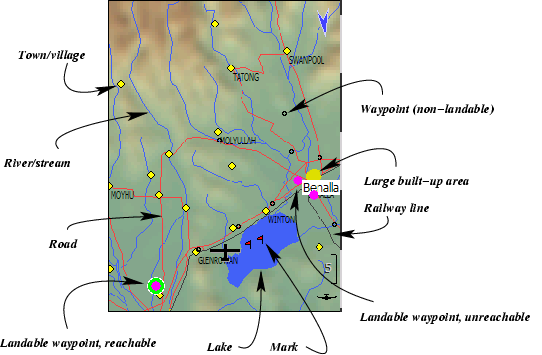
\includegraphics[angle=0,width=\linewidth,keepaspectratio='true']{figures/fig-map.png}
\end{maxipage}

The moving map shows:
\begin{enumerate} 
\item Glider symbol
\item Waypoints
\item The active task
\item The bearing to the next waypoint
\item Special Use Airspace
\item Terrain and topology
\item Markers
\item Trail
\item Glide range
\end{enumerate}
The map is drawn in a projected coordinate system (not latitude and
longitude), and the scale can be changed (zooming in and out), as well
as panned.  All navigation functions take the curvature of the Earth
into account.

\section{Glider symbol, map orientation}
The glider symbol shows the position of the glider on the map.  The
orientation of the glider indicates the estimated heading of the
glider.

The map is oriented in one of two ways, depending on the flight mode
and the configuration settings:
\begin{description}
\item[North-up]  Here the map is always oriented with true north up.
  The glider symbol is rotated according to its track corrected for wind.
\item[Track-up]  Here the map is oriented so that the glider's track
  made good is up.  The north arrow symbol points to true north.  
  The glider symbol may be shown rotated according to the computed
  heading of the glider taking wind into account.
\end{description}

Configuration settings can be used to further specify north or
target-up when in circling mode.  These are useful to prevent
disorientation when looking at the map while circling.  Target-up when
circling makes it easy to determine which direction to exit the
thermal.

When in North or target-up in circling modes, the glider symbol is
centered on the screen.  Otherwise the glider symbol is positioned
20\% from the bottom of the screen, giving a good view of the map
ahead of the glider.  This position is adjustable in the configuration
settings.

A fifth mode has north-up during cruise and track-up in circling.

\section{Zoom and map scale}

To change the scale of the map, for PC or Pocket PC:
\begin{enumerate}
\item Tap on a blank part of the map to highlight the map if it is not already selected.
\item Then use the Pocket PC up/down key to either zoom in or out.
\end{enumerate}

On Altair, the rotary knob can be used to zoom in and out, or select
from the menus:
\begin{quote}
\bmenu{DISPLAY}\blink\bmenu{Zoom in} and \bmenu{DISPLAY}\blink\bmenu{Zoom out}
\end{quote}

The map scale is displayed in the lower left corner of the moving map
display, and as a striped bar on the right side of the map area.  The
alternating colours in the striped bar represent the distance
measurement in a decimal scale, (e.g.\ 0.1 km, 1 km, 10 km, 100 km)
depending on the zoom level.
\marginpar{
\includegraphics[angle=0,width=0.4\linewidth,keepaspectratio='true']{figures/zoom.png}}

Compaq Aero Users. If you enable the Compaq Aero Game Keys (On the
Q-menu) the centre two front buttons become the up/down keys.

There is a facility to have two zoom settings; one when the glider is
in circling flight mode, and one in the cruise or final glide flight
mode.  This is the "Circling zoom" option in the configuration
settings.  
%By default, the cruise/final glide zoom is 5 km and the
%circling zoom is 0.3 km.
%\marginpar{XXX TODO Check these}
When the user zooms in or out, it affects the current
mode's zoom setting only, so when leaving the mode the previous mode's
zoom setting is used.  If `Circling Zoom' is not enabled, there is
only a single zoom level.

Auto-zoom automatically zooms in when approaching a waypoint to keep
the waypoint at a reasonable screen distance.  The user can still zoom
out if desired.  When auto-zoom is active, 'AUTO' appears next to the
map scale.  
\marginpar{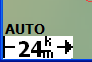
\includegraphics[angle=0,width=0.4\linewidth,keepaspectratio='true']{figures/zoomauto.png}}

To turn auto zoom on or off, select from the menu
\begin{quote}
\bmenu{DISPLAY}\blink\bmenu{Zoom Auto} 
\end{quote}

When a waypoint changes (automatically, via the task selector, or by
manually switching waypoints), auto-zoom returns the zoom level to what
it was immediately prior to its alteration.  This has the effect of
allowing users to zoom in and out manually in cruise, and when
approaching a waypoint, the system automatically zooms in.  When
passing the waypoint, the system goes back to the previous cruise zoom
level in effect.

%\begin{center}
%
%{\it DIAGRAM SHOWING MAP SCALE AND AUTOZOOM SYMBOL (CUTOUT OF MAIN MAPAREA)}
%\end{center}
%
%{\it DIAGRAM SHOWING HOW AUTOZOOM WORKS AS YOU APPROACH AND PASS A WAYPOINT}

\section{Panning the map}

A pan mode allows the user to explore areas beyond the glider.  This
is particularly useful when task planning.
\begin{enumerate}
\item Enable pan mode by pressing 
\begin{quote}
\bmenu{DISPLAY}\blink\bmenu{Pan}
\end{quote}

\item The map can then be panned by dragging the screen or using the cursor
  keys.  For Altair, panning is performed with the inner/outer rotary knob.
\item When done, pan mode should be disabled, by activating the menu again:
\begin{quote}
\bmenu{DISPLAY}\blink\bmenu{Pan}
\end{quote}

\end{enumerate} 

When pan is active, the text 'PAN' appears next to the map scale.  The
location of focus moves and rotates with the glider when panning.  

A special menu of buttons in pan mode is also displayed when in pan
mode.

\begin{center}
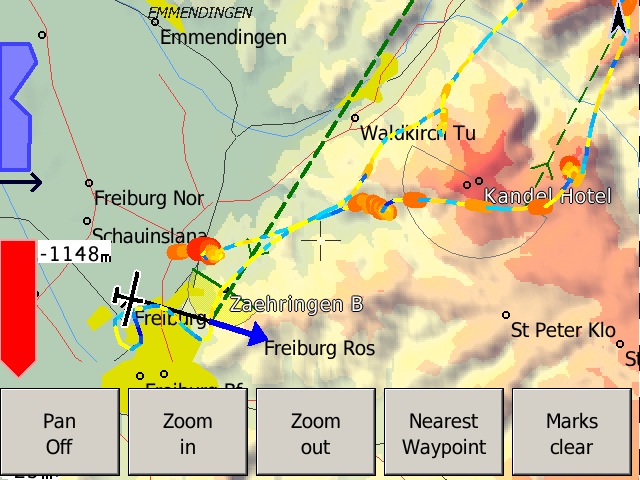
\includegraphics[angle=0,width=\linewidth,keepaspectratio='true']{figures/pan.png}
\end{center}

\section{Waypoints}
Waypoints are displayed with different symbols depending on the
waypoint type; the major distinction being landable and non-landable
waypoints.

The waypoint symbols are drawn as shown below:
\begin{itemize}
\item Non-landable waypoints are small black hollow circles.
\item Unreachable airfields are purple filled circles.
\item Reachable airfields in purple filled circles with a green band.
\end{itemize}
At large zoom scales, all waypoints are drawn as small black crosses.

%\begin{center}
\marginpar{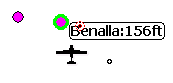
\includegraphics[angle=0,width=\linewidth,keepaspectratio='true']{figures/cut-waypoints.png}}

%{\it DIAGRAM SHOWING DIFFERENT WAYPOINT SYMBOLS ON A MAP: NORMAL WAYPOINTS, 
% LANDABLE AIRFIELDS, REACHABLE LANDABLE AIRFIELDS.  FULLSCREEN, NO TASK}
%\end{center}

Waypoints are optionally labelled according to one of several
abbreviation schemes.

XCSoar continually calculates which landing points are within gliding
range using the current wind estimate.  The estimated arrival altitude
{\em above the arrival safety height} of reachable landable points is
optionally displayed next to the waypoint (see
Section~\ref{sec:map-display} for these configuration options).  This
arrival altitude is calculated at the MacCready setting of zero.

\section{Active task}

The active task course is drawn on the map as a green dashed line.
Assigned area tasks also show the task sectors or areas as a shaded
region.  The start and finish waypoint additionally show black circles
and grey lines representing the start and finish zones or lines.
Circles are always drawn around start and finish points, lines are
only drawn if the start/finish points are of line type.  Task
observation sectors are drawn as segments.

At all times a thick black line is drawn from the glider to the next
waypoint in the task.

\begin{center}

\begin{tabular}{c c c}
{\it Start/finish} & {\it Sector} & {\it Barrel} \\
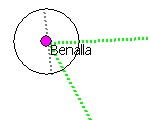
\includegraphics[angle=0,width=0.3\linewidth,keepaspectratio='true']{figures/cut-startfinish.png} &
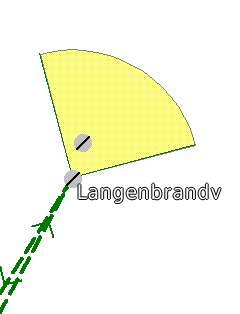
\includegraphics[angle=0,width=0.3\linewidth,keepaspectratio='true']{figures/cut-sector.png} &
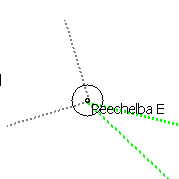
\includegraphics[angle=0,width=0.3\linewidth,keepaspectratio='true']{figures/cut-barrel.png} \\
\end{tabular}
\end{center}

\section{Terrain and Topology}

The following topological features are drawn on the map:
\begin{itemize}
\item Major roads, shown as red lines
\item Rivers, shown as blue lines
\item Large water bodies (lakes), shown as blue areas
\item Large cities, shown as yellow areas
\item Small population areas, shown as yellow diamonds
\end{itemize}
Cities and small population areas are labeled in italics.

Terrain is coloured according to height, and optionally shaded by sun
direction or lift-generating slope.  Invalid terrain, or terrain below
sea level is coloured blue.

Terrain is phong-shaded to improve visibility.  Currently the shading
is set up so that the virtual lighting position is the wind bearing,
thus brighter areas are on the upwind side of hills and dark areas in
the lee of the hill.  The amount of phong shading and overall terrain
brightness is configurable.  Support for a sun ephemeris is underway.
Terrain shading and brightness can be adjusted in the configuration
settings.

Both terrain and topology display can be switched on or off from the
menu:
\begin{quote}
\bmenu{DISPLAY}\blink\bmenu{Terrain toggle}
\end{quote}

\begin{center}
\begin{tabular}{c c}
Topology & Terrain \\
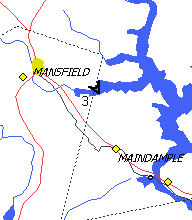
\includegraphics[angle=0,width=0.4\linewidth,keepaspectratio='true']{figures/cut-topo.png} &
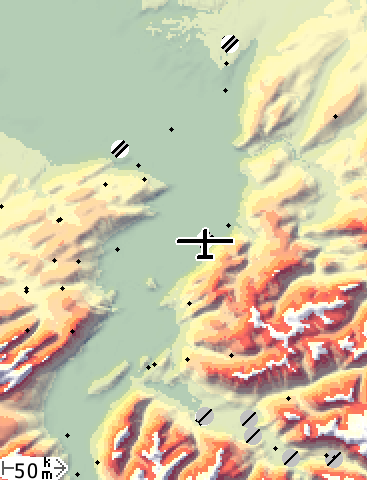
\includegraphics[angle=0,width=0.4\linewidth,keepaspectratio='true']{figures/cut-terrain.png} \\
\end{tabular}

%{\it DIAGRAMS SHOWING TOPOLOGY AND TERRAIN, SHADING. FULLSCREEN, NO TASK}
\end{center}

If the terrain file is not specified (or terrain display is turned
off), the background colour of the map window is white.  All terrain
below mean sea level is coloured blue.  If you are flying outside the
terrain region, the background colour will also be blue.

The screen can be de-cluttered, turning off the display of topology
labels and non-task waypoint labels by toggling:
\begin{quote}
\bmenu{DISPLAY}\blink\bmenu{Declutter labels}
\end{quote}


\section{Trail}\label{sec:trail}

An optional 'snail trail' is drawn on the map showing the glider's
path history.  The colour and thickness of the trail depends on the
variometer value; with lift areas being presented in green and thicker
lines, sink areas being presented in red with thin lines.  Zero lift
is presented as a grey line.

\begin{center}
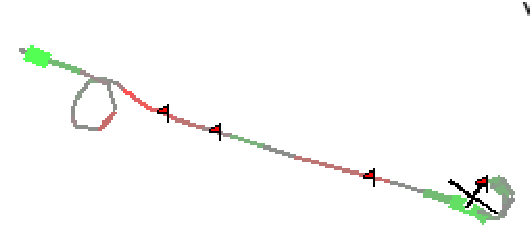
\includegraphics[angle=0,width=0.8\linewidth,keepaspectratio='true']{figures/snail.pdf}
\end{center}

If Vega or an intelligent variometer is connected with Netto output,
the Netto vario value is used; hence the colours and thickness of the
trail indicates the air-mass vertical movement rather than the glider's
vertical movement.

The snail trail display can be toggled between off, a short trail
(about ten minutes), a long trail (about one hour) or a full trail
which displays the entire flight.  This can be performed permanently
through the configuration settings or temporarily by the menu:
\begin{quote}
\bmenu{DISPLAY}\blink\bmenu{Snail trail}
\end{quote}

Note that each of these all modes, the snail trail is short in
circling mode in order to reduce screen clutter.

In order to assist centering thermals in the presence of wind, the
snail trail can be artificially drifted with the wind as it is
displayed (this is drift compensation).  In this way, the snail trail
is referenced to the prevailing wind rather than referenced to the
ground.  Since thermals drift with the wind also, the drifted trails
give a better indication of where the glider has been relative to the
thermals.

An example of this is illustrated below.  Note that when trail drift
compensation is active (right picture), the glider appears to be
circling in a column rather than an elongated spiral (left picture).

\begin{center}
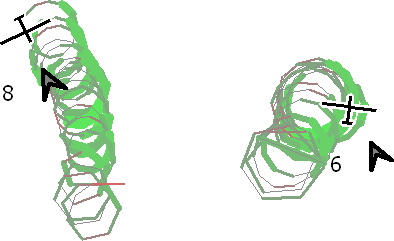
\includegraphics[angle=0,width=0.8\linewidth,keepaspectratio='true']{figures/traildrift.png}
\end{center}

Enabling trail drift compensation is performed through the
configuration settings.  The compensation is only performed whilst in
circling mode; the display of the trail in cruise mode is unaffected.
This can also be performed from the wind settings dialog:
\begin{quote}
\bmenu{CONFIG}\blink\bmenu{Setup Wind}
\end{quote}

The trail drift display is useful also to show more clearly when thermals
are cranked due to wind shear.

The trail width can be adjusted in the configuration settings (see
Section~\ref{sec:map-display}).

\section{Markers}

Markers are shown as small flags on the map.  The markers can be dropped
manually, by pressing a button, or automatically.  An example use of
automatic markers is to drop markers when entering circling mode, as a
simple way of showing all thermals encountered.

Markers are not preserved after XCSoar is exited, however the location
of all marks are appended to the file \verb|xcsoar-marks.txt|.

Markers are dropped by the menu: 
\begin{quote}
\bmenu{DISPLAY}\blink\bmenu{Mark drop}
\end{quote}

\section{Glide range line}

A reachable glide `footprint' is displayed on the map display as a
dashed line, indicating where the glider would descend through the
terrain clearance height.  This glide range line is calculated for
tracks extending in all directions.  This feature is useful in
assessing range with respect to topology when searching low for lift,
and when flying in mountainous areas.

\begin{center}
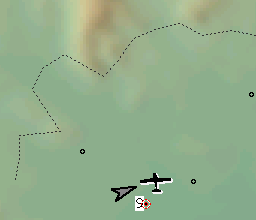
\includegraphics[angle=0,width=0.7\linewidth,keepaspectratio='true']{figures/cut-footprint.png}

%{\it DIAGRAM CUTOUT SHOWING GLIDE RANGE FOOTPRINT.  NO TOPOLOGY,
%FULLSCREEN, NO TASK.}

\end{center}

The final glide path is checked for whether the glider clears terrain
by the terrain clearance height.  If clearance is not attained, a red
cross appears on the map at the point where the violation occurs.  No
icon is drawn if there is no task defined.

\begin{center}
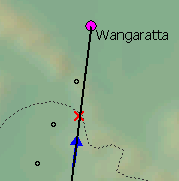
\includegraphics[angle=0,width=0.6\linewidth,keepaspectratio='true']{figures/cut-fgtt.png}
%
%{\it DIAGRAM CUTOUT SHOWING FINAL GLIDE THROUGH TERRAIN WARNING
%SYMBOL.  NO TOPOLOGY, FULLSCREEN, FINAL GLIDE TASK}
%
\end{center}

\section{Status dialog}\label{sec:aircr-stat-dial}

The nearest landmark function, typically available via the button
menu, brings up a status message describing the name, distance and
bearing to the nearest landmark.  The nearest landmark is also
reported on the status dialog.

You may find this function useful when you need to report your
location to others.

Currently the landmarks scanned are the list of waypoints.  In the
future, XCSoar may also search for nearby towns and cities in the
topology database.

The aircraft status dialog (see Section~\ref{sec:dialog-windows})
shows the status of the aircraft's locality, and can be useful when
giving position reports.

This is accessed via the menu under: 
\begin{quote}
\bmenu{INFO}\blink\bmenu{Status}.
\end{quote}
and then selecting the page `Aircraft'.

%%%%%%%%%%%%%%%%%%%%%%%%%%%%%%%%%%%%%%%%%%%%%%%%%%%%%%%%%%%%%%%%%%%%%
\chapter{Cross Country Tasks}\label{cha:tasks}

XCSoar provides a full task management system, in which tasks can be
edited prior to flight and, when undertaking casual cross-country
flying, modified during flight.  Waypoints are advanced automatically
or may be cycled through manually.  This chapter also describes the
use of IGC loggers with XCSoar.

\section{Editing tasks}

You can edit tasks in several ways.  Some methods are more useful for
editing prior to flight, and others allow tasks to be modified whilst
in flight for casual cross-country touring.  Tasks can be saved to
files and loaded later, and can be transferred between any XCSoar
platform (Pocket PC, Altair, PC).

\tip It is also possible to save a `default' task and have this task loaded
automatically upon start-up of XCSoar.  One application of this is to
set up a default task with one waypoint being the home --- this means
that XCSoar is then programmed for final glide back to home, which is
useful for casual cross-country touring.

The main ways of setting tasks are the following:
\begin{itemize}
\item Using the task editor dialog
\item Selecting waypoints from the map and adding them to the task from the
 waypoint details dialog
\item Loading the task from a file
\end{itemize}

%Selecting the Task menu item will produce the Task dialog box.  The
%list box on the left displays all of the turn points loaded into the
%system. Highlight the desired entries and using the "-$>$" and "$<$-"
%buttons assemble the desired task in the Task list box. As each turn
%point is added to the task a continuous display of the calculated task
%length is shown.  Tasks can be saved for recalling later using the
%"Save" button and recalled using the "Load" button.  Once the desired
%task is complete select "OK".
%
%{\it DIAGRAM SHOWING TASK DIALOG EDITING, WITH LABELED ARROWS POINTING
%TO THE USER INTERFACE ELEMENTS?}

\tip Loading a task from file may be useful in competition or casual
cross-country flying in groups, as one person can distribute the task
file to others, thereby saving the group the job of editing the task
themselves.

\tip If no task is present at startup, a task is created automatically,
  containing one waypoint to home.

XCSoar saves the current task when shutting down and loads it at
startup, thereby allowing the task to be entered early in the day,
then turning off the glide computer until ready for flight.

As of version 5.1.2, task waypoints are preserved even if the waypoint
file is changed.  This means, if you save a task, then change the
waypoint file, then load the task again, new waypoints are generated
for any waypoints that are missing in the new waypoint file.

\section{Waypoint details dialog}
%Several ways of selecting a waypoint are available:
%\begin{itemize}
%\item Touch its name or the waypoint symbol on the map screen if it is visible.
%\item If the waypoint is in the active task, highlight the waypoint {\InfoBox}, then use the up/down arrow keys to select the desired waypoint, and press the
%enter key.
%\item From the Task dialog, find and highlight the waypoint in
% the waypoint list, then press the 'Details' button.
%\end{itemize}
%The display will now show the waypoint details dialog.

The waypoint details dialog describes a waypoint in detail and has
navigation functions such as GOTO, Insert.

This may be accessed several ways:
\begin{itemize}
\item
From the task editor, menu \bmenu{NAV}\blink\bmenu{Task Edit} and select
a waypoint, then select the \button{Details} button.

\item 
From the menu \bmenu{INFO}\blink\bmenu{Waypoint details} to show the
details for the active waypoint.

\item
From the menu \bmenu{INFO}\blink\bmenu{Nearest waypoint} to show the
details of the waypoint nearest the aircraft, or if in pan mode,
nearest the pan cursor.

\item
From the waypoint selector, menu \bmenu{NAV}\blink\bmenu{Waypoint
look-up} and select a waypoint to show the details of that waypoint.
\end{itemize}

The waypoint details dialog contains several pages (accessed via the
\button{$>$} and \button{$<$} buttons).

Depending on the configuration files specified in the settings, not
all of these pages may be available.

\subsection*{Waypoint details}
This page contains text describing the waypoint's location, elevation
and local sunset.  
\begin{center}
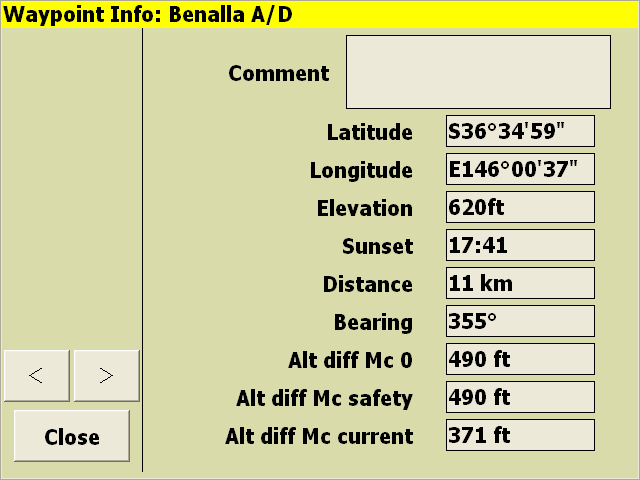
\includegraphics[angle=0,width=\linewidth,keepaspectratio='true']{figures/dialog-waypointdetails0.png}
\end{center}

This page also shows three forms of altitude difference (additional
altitude required to reach the waypoint at the safety altitude) for
the corresponding waypoint:
\begin{description}
\item[Alt diff Mc 0] Altitude difference at Mc setting of 0
\item[Alt diff Mc safety] Altitude difference at the abort/safety MacCready setting
\item[Alt diff Mc current] Altitude difference at the current MacCready setting
\end{description}

\subsection*{Task menu}  
This page contains a column of buttons allowing various actions to be performed:
\begin{description}
\item[\button{Goto (and clear task)}] cancels the current task and sets the waypoint as the
  single active waypoint in the task.
\item[\button{Replace in task}] replaces the active waypoint in the task.
\item[\button{Insert in task}] inserts the waypoint before the active waypoint in
  the task.
\item[\button{Append to task}] adds the waypoint to the end of the task.
\item[\button{Remove from task}] removes the waypoint from the task.
\item[\button{Set as new home}] sets the waypoint as the home airfield.
\item[\button{Set teamcode}] sets the waypoint as reference waypoint for
  team code coordinates.

\end{description}

It is a good idea to set your home waypoint from the waypoint details
dialog. This causes XCSoar to start up at the home location regardless
of whether a GPS fix is received.  If no home is set, then XCSoar
starts in the center of the terrain map.

\subsection*{Airfield information}
This page may contain relevant text from the Enroute Supplement about
the airfield, including runways, radio frequencies, traffic patterns,
contacts.
\begin{center}
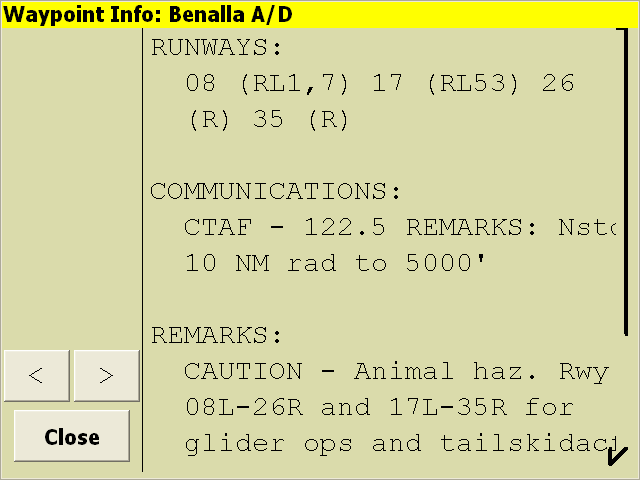
\includegraphics[angle=0,width=\linewidth,keepaspectratio='true']{figures/dialog-waypointdetails1.png}
\end{center}

\subsection*{Satellite image}
This page shows a satellite image of the
waypoint.

\begin{center}
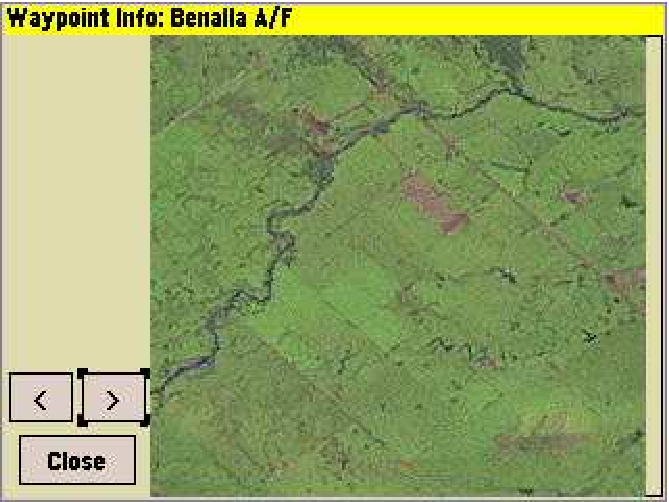
\includegraphics[angle=0,width=\linewidth,keepaspectratio='true']{figures/dialog-waypointdetails2.pdf}
\end{center}


\section{Waypoint selector dialog}
The waypoint selector is a dialog that allows waypoints to be easily selected
from a potentially large database.

This may be accessed several ways:
\begin{itemize}
\item From the menu \bmenu{NAV}\blink\bmenu{Waypoint lookup}
\item From the task editor, menu \bmenu{NAV}\blink\bmenu{Task Edit} and select
 a waypoint, then select the \button{Select} button.
\end{itemize}

The waypoint selector comprises a set of optional filters on the left
side of the page, and a list of matching waypoints on the right.
There are several filters available, which may be used together,
individually or not at all.
\begin{description}
\item[Name] Filtering based on the matching the first letter in the waypoint name. 
\item[Distance] Filters out waypoints further that a specified distance to the aircraft.
\item[Direction] Filters out waypoints that are not in a specified direction from the aircraft. 
   An additional special direction ``HD360'' filters waypoints within 30 degrees to either side of the 
   heading of the glider.  This allows the pilot to point the glider at a group of
  waypoints and quickly find them.
\item[Type] Filters out waypoints that are not of the specified type (Landpoint, Airport or Turnpoint) or
   that appear in the specified File~1 or File~2 (primary or secondary waypoint file respectively).
\end{description}
When filtering by name, the distance and direction filters are reset,
and the list of matching waypoints is sorted by name.  When filtering
by distance or direction, the name filter is reset, and the list
of matching waypoints is sorted by distance.

\begin{center}
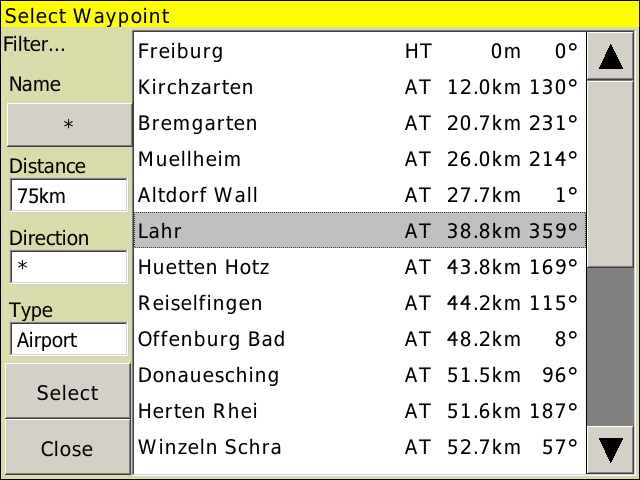
\includegraphics[angle=0,width=\linewidth,keepaspectratio='true']{figures/dialog-waypointselect.png}
\end{center}

The list can be scrolled if there is more than one screen full of
matching waypoints.  To scroll through the list, simply move to the
bottom (or top) of the list with the cursor.  

Pressing the Enter button will select the item in the list under the
cursor.  Selecting an item will result in different behaviour
depending on what function opened the waypoint selector.  In typical
use it brings up the waypoint details dialog for the selected
waypoint.

\section{Task editor dialog}\label{sec:task-editor-dialog}
The task editor is used to edit and view cross country tasks.

This is accessed via the menu
\begin{quote}
\bmenu{NAV}\blink\bmenu{Task Edit}
\end{quote} 

The task editor's primary page is the Task Overview page which
comprises a list of task waypoints on the right side of the form.
Below the list of waypoints, a Total line is displayed that shows
the total distance of the task.
\begin{center}
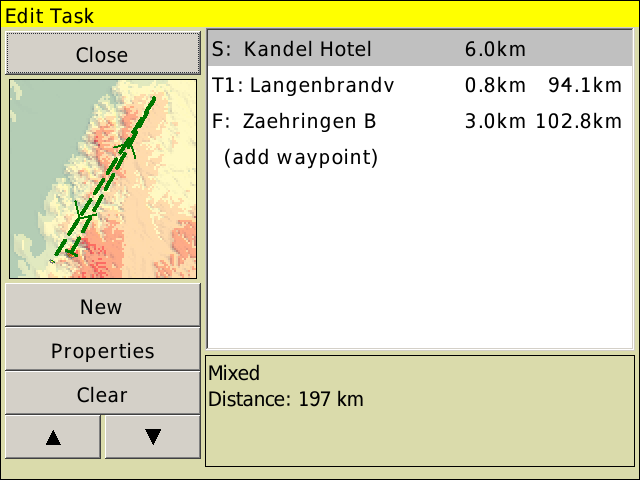
\includegraphics[angle=0,width=\linewidth,keepaspectratio='true']{figures/dialog-taskedit0.png}
\end{center}
The ETE field displays the estimated time on task in minutes for the
current wind estimate and MacCready setting.

For Assigned Area Tasks (AAT) tasks, the Total line displays the AAT
assigned time, the nominal task distance, and the task distance around
the user-specified targets within the AAT areas.

\begin{center}
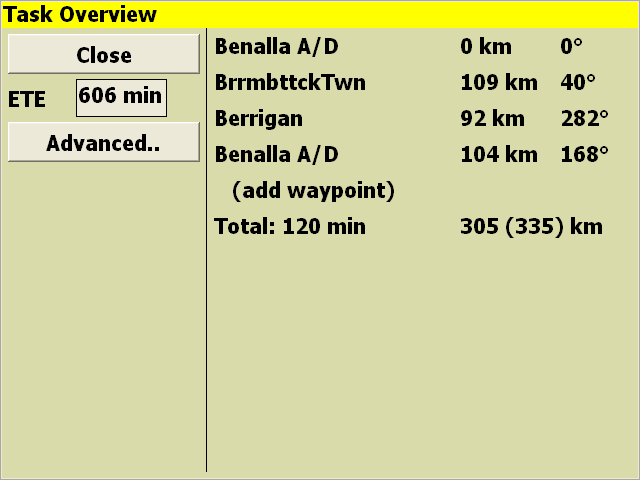
\includegraphics[angle=0,width=\linewidth,keepaspectratio='true']{figures/dialog-taskedit1.png}
\end{center}

Pressing the \button{Advanced} button exposes (or hides) several more
fields.  Pressing it again hides the fields.
\begin{description}
\item[\button{File}] This field defines the task file name to be used by save/load functions.  
\item[\button{Save}] Saves the task to the specified file name.  If a blank file name is selected, then when pressing the Save button, the system will ask for a new file name to be entered.  If the file name already exists, the system will ask the user whether it is OK to over-write the old file.
\item[\button{Load}] Loads the task from the specified file name.
\item[\button{Calc}] Opens the task calculator dialog (see Section~\ref{sec:task-calc-dial}).
\item[\button{Declare}] Sends the task declaration to the logger (if available).
\end{description} 

\begin{center}
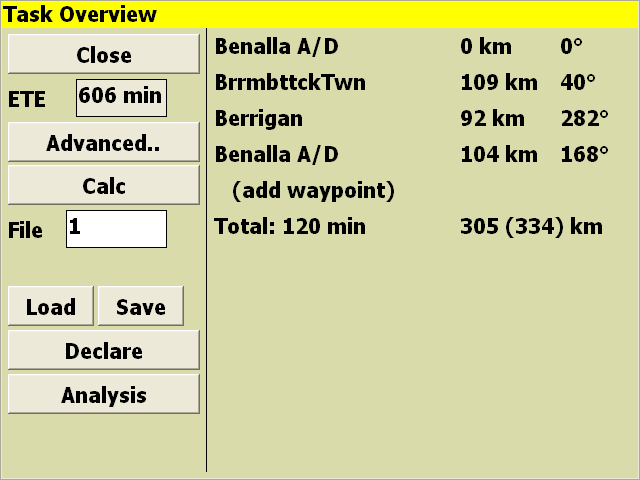
\includegraphics[angle=0,width=\linewidth,keepaspectratio='true']{figures/dialog-taskedit2.png}
\end{center}


Moving the cursor down to a task waypoint in the Task Overview page
and pressing enter will select that waypoint for editing.  New
waypoints can be added to the task by selecting the ``(add new
waypoint)'' line.  Either the home waypoint or start waypoint is
assigned to the new task waypoint, making it quick and easy to define
triangular or out and return tasks.

Once a waypoint is thus selected, a task waypoint dialog appears.
These are different for Start, Turn-point and Finish points.

Each of the task waypoint dialogs have the following buttons on the
left side of the form:
\begin{description}
\item[\button{Close}] Closes the dialog and returns to the task overview page
\item[\button{Select}] Opens the waypoint selector dialog, allowing the waypoint to be
 changed.  If the Close button or ESC button in the waypoint selector
 is pressed, the task waypoint will be unchanged.
\item[\button{Remove}] Removes the waypoint from the task
\item[\button{Details}] Opens the waypoint details dialog to give more detailed information on the waypoint location.  
This can be useful to verify the waypoint coordinates are correct.
\item[\button{Move up}] Moves the waypoint to earlier in the task.
\item[\button{Move down}] Moves the waypoint to later in the task.
\end{description}

The task waypoint dialogs for start points contain several fields:
\begin{description}
\item[Start type] Line or cylinder
\item[Start diameter] Diameter of the cylinder or length of the start line.
\item[Sector type] Sector type (cylinder, FAI sector or German sector) 
 for non-AAT tasks.
\item[Sector radius] Sector radius for non-AAT tasks.
\item[AAT] Determines whether this task is AAT or not.
\item[Min time] Specifies the AAT minimum task time.  During flight, if the expected task time is less than the AAT minimum task time, a status message notificatio of this is issued.
\item[OnLine Contest]  Specifies whether the detection of start is based
  on the start sector or minimum altitude after launch (required for
  Sprint tasks).
\item[Auto advance] Controls the auto advance mode, as described in Section~\ref{sec:advanc-rest-tasks}.
\item[Alternate start points]  Determines whether there are alternate start sectors at other start points as well as this waypoint.
\end{description}

\begin{center}
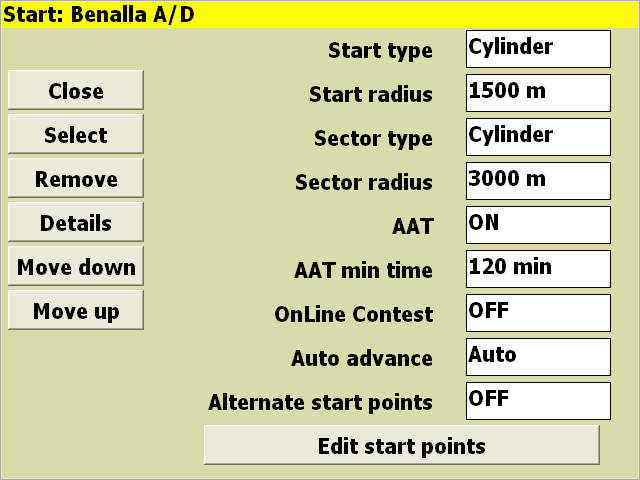
\includegraphics[angle=0,width=\linewidth,keepaspectratio='true']{figures/dialog-taskedit3.png}
\end{center}

The \button{Edit start points} button allows editing of alternate
start points.  See Section~\ref{sec:alternate-starts} for more
details.

The task waypoint dialog for turn-points in non AAT-tasks do not
contain any editable fields.  For both AAT and non AAT tasks, the
finish waypoint dialog allows the finish type to be defined:
\begin{description}
\item[Finish type] Line or cylinder
\item[Finish diameter] Diameter of the cylinder or length of the finish line.
\end{description}


For AAT tasks, the task waypoint dialog for turn-points allows the AAT
areas to be defined.
\begin{description}
\item[Target distance]  This allows the target within the AAT area to be moved to produce the shortest (-100\%) to longest (100\%) task distance.
The use of targets is described further in Section~\ref{sec:aat-tasks}.
\item[Type] Cylinder or sector.
\item[Circle radius] The radius of cylinder in meters for cylinder type.
\item[Sector radius] The radius of the sector in meters for sector type.
\item[Start radial] The start radial of the sector in degrees.
\item[Finish radial] The finish radial of the sector in degrees.
 The convention is that the sector is defined in a clockwise direction from
  start to finish radial.
\end{description}
\begin{center}
\includegraphics[angle=0,width=\linewidth,keepaspectratio='true']{figures/dialog-taskedit4.png}
\end{center}

\section{Advancing and restarting tasks}\label{sec:advanc-rest-tasks}

At all times one waypoint in the task is designated as the active
waypoint.  The active waypoint is used for calculation and display of
navigation information, that is, the pilot is directed to fly towards
the active waypoint (also referred to as the 'next waypoint' in the
description of InfoBoxes as in Chapter~\ref{cha:infobox}).

During flight a continuous display of the bearing of the next turn
point is shown.

The altitude required to complete the task is calculated from the
glider's position to the active waypoint through to the final
waypoint.

Changing the active waypoint can be performed automatically and
manually in the following ways.
\begin{description}
\item[Auto advance mode]
Once the aircraft enters the turn point observation zone and satisfies
the turn point rules, the software will automatically select the next
task turn point.

The active waypoint is advanced through the list of waypoints in the
task automatically: the start waypoint is advanced when the starting
conditions are met (such as flying through a start line or leaving a
start cylinder); intermediate waypoints are advanced when the glider
passes through the observation zone (for AAT tasks, the waypoint is
advanced when the glider enters the AAT area).
\item[Arm auto advance]
This is similar to the Auto method, but it requires the pilot to arm a
trigger.  Therefore, if the advancement conditions are met but the
trigger is not armed, the waypoint is not advanced.  The `Arm' button can be 
used to arm the trigger.  It is accessed via the menu
\begin{quote}
\bmenu{NAV}\blink\bmenu{Arm advance}
\end{quote}
\item[Arm auto advance start]
This is similar to the Auto method but the start must be armed.
Therefore, the pilot must press the arm button before starting, and on
subsequent waypoints the advancement is automatic.
\item[Manual advance]
Fully manual control.  No automatic advancement is performed at all.
\end{description}  

Status messages are given in arm modes (``arm start'' or ``arm''
modes) when inside the observation sector, as reminders to press arm
when the pilot is ready to advance to the next waypoint.
For starting, a warning is given that the glider is in the start
cylinder or behind the start line, as a reminder to ARM if necessary.

In all auto advance modes, the pilot can adjust the current waypoint
with the buttons:

\begin{quote}
\bmenu{NAV}\blink\bmenu{Waypoint next} and \bmenu{NAV}\blink\bmenu{Waypoint previous}
\end{quote}

For PC and Pocket PC with touchscreen versions only, the user may
manually cycle through the waypoints by highlighting the waypoint
{\InfoBox} and by pressing the up or down cursor key.

See Section~\ref{sec:task-rules} for details on observation rules.

If a user has cycled through the waypoint manually, this does not mean
that the glider has successfully passed the waypoint!  However, this
facility is useful to force a task restart or to skip a waypoint when
flying a casual cross-country task.

\tip Tasks can be restarted simply by manually cycling back through the
waypoints to the start.

In all modes, if the glider re-enters the start zone or crosses the
start line within 10 minutes of the previous start, the task may be
automatically restarted.  In ARM and ARM Start modes, the pilot still
needs to activate ARM to re-start.

When selecting 'previous waypoint', the trigger that detects
auto-advance for that waypoint is cleared; meaning that the task
computer expects the aircraft wants to fly to that observation zone
again before continuing the task.  The pilot may still select 'next
waypoint' to advance to the next task waypoint.

A system beep and message is given on task/waypoint advance.  The
messages are given when the system advances the task waypoint
automatically or, in arm modes, when the system is armed and the
aircraft is in sector:
\begin{itemize}
\item[Task start] appears when the aircraft has crossed the start line or
 exited the start sector; if the advance system is automatic, or for
 arm modes, if the system is armed.  For arm modes, if the aircraft
 has already crossed the start line or exited the start sector,
 pressing arm will cause the message to appear to confirm a valid
 start.
\item[Next turnpoint] appears when the aircraft has entered the observation
 sector for turnpoints; if the advance system is automatic, or for arm
 mode, if the system is armed.  For arm modes, if the aircraft has
 already entered the observation sector and left, pressing arm will
 cause the message to appear to confirm a valid advance to the next
 turnpoint.
\item[Task finish] appears when the aircraft has crossed the finish line
 or entered the finish cylinder.  This occurs in all advance modes. 
\end{itemize}

\section{Task rules}\label{sec:task-rules}

A variety of task rules may be used when specifying tasks, including
the common FAI triangles and Assigned Area Tasks (AAT).  Many aspects
of the rules can also be customised.

Starting and finishing lines are centered on their associated waypoint
and aligned perpendicular to the next and previous waypoints
respectively.

Sector turn-points are 90 degree segments aligned to the bisection of
the previous and next waypoints, as commonly used in FAI tasks.
There is also support for German DAe sectors.

Automatic advancement of the start task depends on the type of start:
\begin{description}
\item[Cylinder] When the glider leaves the cylinder area.
\item[Line] When the glider crosses the start line.
\item[FAI 90 sector] When the glider crosses the start sector lines.
\end{description}

Automatic advancement of intermediate waypoints depends on their type:
\begin{description}
\item[FAI Sector] When the glider has entered the observation zone, defined 
by a segment and radial distance from the waypoint.  The segment is
defined by a 90 degree arc centered about the bisector of inbound and
outbound legs, with a distance of 20 km.
\item[DAe 0.5/10 sector] When the glider has entered the observation zone, 
defined by a segment and radial distance from the waypoint.  The segment is
defined by a 90 degree arc centered about the bisector of inbound and
outbound legs, with a distance of 10 km.  The observation zone also includes
a cylinder of 500 m.
\item[Cylinder]  When the glider has entered the observation zone defined
by a radial distance from the waypoint.
\item[AAT] When the glider has entered the observation zone defined by the
radial distance from the waypoint, and segment for sector areas.
\end{description}

Task completion depends on the finish type:
\begin{description}
\item[Cylinder] When the glider enters the cylinder area.
\item[Line] When the glider crosses the finish line.
\end{description}

\tip Competition rules may be defined in a profile file for
distribution to a group of pilots or task-setters, so all competitors
are playing by the same rules!

Additional task rules for valid starts and finishes may also be
specified.  Starts may have a defined maximum altitude above ground,
and a maximum speed.  Finishes may have a minimum altitude above
ground.  These parameters are defined in the page ``Task Rules'' in
the configuration settings.  If any of the values are zero, the
corresponding limit rule is not applied.

For non-AAT tasks, an option is available to set the minimum finish
altitude according to the FAI rule, whereby the minimum finish
altitude is above 1000 meters below the start altitude.

\section{Alternate starts}\label{sec:alternate-starts}

The task system allows alternate start sectors to be defined.
  
To use it, on the task edit page, select the start point, then turn on
the `Alternate start points' property.  Then press the button 'Edit
alternate start points'.

\begin{center}
\includegraphics[angle=0,width=\linewidth,keepaspectratio='true']{figures/dialog-startpoint2.png}
\end{center}
  
  To edit the start points, move the cursor to an item in the list on
  the right side of the dialog, and press enter.  This opens the
  waypoint selector dialog, to allow selection of the waypoint.  This
  process can be repeated several times for several alternate start
  waypoints.  Press the `clear' button to clear all alternate start
  points.

  Each start sector is fixed to the same type (line/cylinder) and size
  (start radius) defined in the task waypoint page.

  Note that the task start point should be included in the alternate
  start location list. 

\begin{center}
\includegraphics[angle=0,width=\linewidth,keepaspectratio='true']{figures/dialog-startpoint3.png}
\end{center}

\begin{center}
\includegraphics[angle=0,width=\linewidth,keepaspectratio='true']{figures/dialog-startpoint4.png}
\end{center}

  In flight, any time you cross a start line (or exit a start
  cylinder), this will start the task at that particular alternate
  start.  Task statistics are recalculated for the start sector you
  last flew through.  All alternate start sectors are shown on the
  map.  You can re-start simply by flying through the start sector
  again or another start sector.  This automatic re-start will only
  happen if the active waypoint is the first turnpoint after the
  start, or the start itself.

  When the waypoint advance mode is `Arm' or `Arm Start', then a start
  is only recognised by XCSoar if the advance trigger is armed.

  If desired, alternate start points may be selected as the active
  waypoint by selecting the previous waypoint.  Continuing to select
  the previous waypoint will cycle through all alternate start points.

\section{Task calculator dialog}\label{sec:task-calc-dial}
The task calculator dialog allows the pilot to see the effect of
various changes to the task on final performance.

This may be accessed several ways:
\begin{itemize}
\item From the menu 
\begin{quote}
\bmenu{NAV}\blink\bmenu{Task calc}
\end{quote}
\item From the task editor, menu \bmenu{NAV}\blink\bmenu{Task Edit} and select
 the button \button{Advanced} then \button{Calc}
\item From the analysis dialog, menu \bmenu{INFO}\blink\bmenu{Analysis} and select
 the button \button{Calc}
\end{itemize}

\begin{center}
\includegraphics[angle=0,width=\linewidth,keepaspectratio='true']{figures/dialog-taskcalc3.png}
\end{center}

\begin{description}
\item[Assigned task time]  This field displays the assigned task time.
\item[Estimated task time]  This field displays the estimated total time 
 on task to complete the task at the provided MacCready setting.
\item[Task distance]  This field displays the task distance remaining.
\item[Set MacCready]  Allows the user to adjust the MacCready value and 
 see the effect it has on the estimated task time.
\item[Set range]  Allows the user to adjust the targets within the remaining 
 AAT areas, to see the effect it has on estimated task time and task distance.
\item[Set speed remaining]  This field displays the estimated speed for the
 remainder of the task at the provided MacCready setting.
\item[Achieved MacCready]  This field displays the achieved MacCready value.
\end{description}
See Section~\ref{sec:task-speed-estim} for more details on task speed
and achieved MacCready calculations.

If the \button{OK} button is pressed, the value entered in the ``Set
MacCready'' field is used as the MacCready setting.  If the
\button{Cancel} button is pressed, the MacCready setting is
unaffected.

The \button{Optimise} button, for AAT tasks, adjusts the range
(increases or decreases) so that the estimated task time exceeds the
assigned task time by less than five minutes.  In typical use, using
this button means the pilot does not have to manually adjust the range
to find the course for arrival at the assigned task time, thereby
reducing pilot workload.

\section{Task status dialog}

The status dialog (see Section~\ref{sec:dialog-windows}) gives a
summary of important task information.  It can be useful to give a
good overview of the task status while freeing up InfoBoxes for other
purposes.  The status dialog can be referred to in order to confirm
that a valid start was detected, as well as the progress against the
task.

This is accessed via the menu:
\begin{quote}
\bmenu{INFO}\blink\bmenu{Status}
\end{quote}
and then selecting the page `Task', or `Rules'.

\section{Assigned Area Tasks}\label{sec:aat-tasks}

\subsection*{AAT targets}

A {\em target} is a point within an AAT area that the pilot intends to
fly to.  These targets can be moved within the AAT areas so the pilot
can adjust the effective distance of the task.  Targets may be set on
the ground, during task planning, and modified during flight.

When flying an AAT task, the navigation system directs the glider to
the target, and statistics like distance to waypoint are also relative
to the target rather than the waypoint of the AAT area itself.

Automatic task waypoint advancement normally triggers when entering an
AAT area, so if the pilot wishes to fly to the targets, either the
`arm start', `arm' or `manual' advancement modes should be used when
flying AAT tasks.  See Section~\ref{sec:advanc-rest-tasks} for
details.

\subsection*{Manually moving targets}

In order to make the specification of targets more straightforward,
their location is defined by a range parameter that determines how
far from the minimum to maximum possible distance the target is.  This
is expressed as a percentage.  For example, with range set to 100\%,
the target is located to give the maximum overall task distance.  With
range set to~$-100$\%, the target is located to give the minimum overall
task distance.  

Zero range yields a nominal task distance: for sectors the target is
half way along the bisector radial; for cylinders the target is in the
center of the cylinder.

The targets can be modified in two ways:
\begin{itemize}
\item From the task calculator dialog (see 
 Section~\ref{sec:task-calc-dial}), the \button{Range} field adjusts the
 targets of all remaining waypoints in the task.
\item From the task editor dialog (see 
 Section~\ref{sec:task-editor-dialog}), the range of each waypoint may
 be individually adjusted.
\end{itemize}

\subsection*{AAT targets and the Task Calculator}

The typical use of targets in flying AAT is as follows:
\begin{itemize}
\item Set the expected MacCready, bugs/ballast and wind settings
  for the flight using the basic settings and wind settings dialogs.
\item Define the task as normal from the task editor.
\item Based on the pilot's judgement of how good the weather is,
  and whether some areas are likely to me more or less difficult than
  others, targets may be set individually for each turn-point in the
  task editor.  The ETE field in the task editor can be compared to
  the assigned minimum time to check the planned task is efficient and
  long enough.
\item During flight, if situations change, such as changed MacCready setting
  or wind, the task calculator can be brought up to show the estimated
  task time, again allowing comparison to the assigned minimum time.
\item If the pilot decides to extend or shorten the flight, all the remaining
  targets can be modified from the task calculator. 
\end{itemize}

The task calculator therefore allows the pilot to make (and help to
answer) `what if?' questions, for example:
\begin{itemize}
\item What will happen if the conditions improve?  The MacCready setting can be increased and the pilot can see if there is sufficient adjustment to targets in order to be able to extend the planned task.
\item What will happen if the conditions deteriorate?  The MacCready setting can be decreased and the pilot can see how much the task can be shortened and still finish the task later than the assigned minimum time.
\item What will happen if I leave the AAT area now?
%XXX TODO: need a bit more functionality here.
\end{itemize}

\subsection*{Target projection}

XCSoar continually analyses the path of the glider through AAT sectors
to find the points in previous AAT sectors through which the achieved
scoreable distance will be greatest.  Internally, the program moves
the targets for previous AAT sectors, which are then the optimal
targets.

In certain conditions, targets for the current AAT sector may be moved
automatically:
\begin{itemize}
\item When inside an AAT sector, the target in that sector is moved to
to a line projecting from the previous sector's target through the
aircraft, at the same distance from the previous sector's target to
the target prior to entering the sector.  The effect of this is to
allow pilots to choose to enter an AAT sector in a different direction
or offset from the direct line from the previous target to the current
target.

\item While the aircraft is in the AAT sector and the distance from the
previous target to the aircraft is greater than the distance from the
previous target to the current target, the target is moved further
along the projected line from the previous target to the aircraft,
just beyond the aircraft.  Hence, the black track line will not be
visible but the blue optimal track arrow will point along this
projected direction.
\end{itemize}

A worked example is provided in the following figures to illustrate
how targets move during a flight and to show how XCSoar determines the
maximum scored path.

\begin{maxipage}
\begin{center}
\begin{longtable}{|c|c|}
\toprule
\includegraphics[angle=0,width=0.45\linewidth,keepaspectratio='true']{figures/faat01.png} & 
\includegraphics[angle=0,width=0.45\linewidth,keepaspectratio='true']{figures/faat02.png} \\
{\em Outside sector} & {\em Inside sector} \\
Target (-20\%) is on bisector & Target moved along track line \\
 \midrule
\includegraphics[angle=0,width=0.45\linewidth,keepaspectratio='true']{figures/faat03.png} & 
\includegraphics[angle=0,width=0.45\linewidth,keepaspectratio='true']{figures/faat04.png} \\
{\em User decreased range} & {\em User increased range} \\
Target (-80\%) moved along track line & Target (80\%) moved along track \\

 \midrule

\includegraphics[angle=0,width=0.45\linewidth,keepaspectratio='true']{figures/faat05.png} & 
\includegraphics[angle=0,width=0.45\linewidth,keepaspectratio='true']{figures/faat06.png} \\
{\em Analysis (task page)} & {\em Next waypoint} \\
Path around active target  & Arm advance pressed \\
\bottomrule
\end{longtable}
\end{center}
\end{maxipage}

\begin{maxipage}
\begin{center}
\begin{longtable}{|c|c|}
\toprule
\includegraphics[angle=0,width=0.45\linewidth,keepaspectratio='true']{figures/faat07.png} & 
\includegraphics[angle=0,width=0.45\linewidth,keepaspectratio='true']{figures/faat08.png} \\
{\em Analysis (task page)} & {\em Approaching next area} \\
Best scored target found & Target (60\%) is on bisector \\

 \midrule

\includegraphics[angle=0,width=0.45\linewidth,keepaspectratio='true']{figures/faat09.png} & 
\includegraphics[angle=0,width=0.45\linewidth,keepaspectratio='true']{figures/faat11.png} \\
{\em Inside sector} & {\em Next waypoint} \\
Target (60\%) moved along track line & Arm advance pressed \\

 \midrule

\includegraphics[angle=0,width=0.45\linewidth,keepaspectratio='true']{figures/faat12.png} &  \\
{\em Analysis (task page)} &  \\
Best scored targets found &  \\
\bottomrule
\end{longtable}
\end{center}
\end{maxipage}

\section{OnLine Contest}

  The analysis dialog contains a page `OnLine Contest' which can be
  used to show the optimal path and estimated score.  The
  configuration settings (task rules page) allows the selection of
  which set of rules to be used for the OLC optimisation:
\begin{description}
\item[Sprint] Conforms to FAI IGC League rules.  Up to 5 points including start and finish, maximum duration 2.5 hours, finish height must not be below start height.
\item[Triangle] Conforms to FAI OLC triangle rules.  Four points with common start and finish.  For tasks longer than 500km, no leg less than 25\% or larger than 45\%; otherwise no leg less than 28\% of total.  Finish height must not be lower than start height less 1000 meters.
\item[Classic] Conforms to OLC classic rules.  Up to seven points including start and finish, finish height must not be lower than start height less 1000 meters.  Points awarded 80\% on second last leg and 60\% on last leg.
\end{description}

  The Sprint rules require the start altitude to be the lowest
  altitude in the flight after release from tow.  The detection
  of this start point can be enabled in the task editor, selecting the
  start point and turn `OLC' to ON.

\begin{center}
\includegraphics[angle=0,width=\linewidth,keepaspectratio='true']{figures/shot-olc.png}
\end{center}

  When flying OLC, either AAT or non-AAT tasks may still be used to
  manage the flight navigation.  During flight, if the `Optimise'
  button in the OLC page of the analysis dialog is pressed, the
  computer will optimise the current flight with respect to the
  selected OLC rules.  

  In the OLC analysis page, the aircraft track is shown as a thin
  green line, and after optimisation, the optimal path is shown as a
  thick red dashed line.

  If continued flight in final glide will result
  in higher score, the displayed results are shown as `In progress'
  and a blue line shows the projected path to improve the score.
  For Sprint and Classic OLC types, this path is extended in the direction
  to the current waypoint.  For Triangle OLC type, this path is extended
  in the direction to produce the largest triangle.

  The score and computed optimal distance is approximate.

  If continued flight in final glide will not achieve a higher score,
  or if the aircraft has landed, the displayed results are shown as
  `Finished'.  

  Depending on the duration of the flight, the time required to
  calculate the optimum path may take up to 10 seconds.

\section{Abort/resume task}

If atmospheric conditions change for the worse, you may make the
judgement that it will be impossible to complete the task.  In this
situation, XCSoar can be instructed to 'abort' the task, and it will
then help you reach a safe landing site.

To abort/resume the task, press
\begin{quote}
\bmenu{NAV}\blink\bmenu{Abort task}
\end{quote}

When in abort mode, whatever cross-country task was being flown is
discarded.  The task waypoint list is then filled with nearby landing
points, ordered by the estimated arrival altitude at best glide angle
with the safety MacCready ring setting, adjusted for wind.  The
first waypoint in the list is therefore the most reachable waypoint.

The configuration option `Abort use current Mc' determines whether
waypoint arrival heights in abort mode uses the MacCready value prior
to aborting the task, or if the safety MacCready value is used.  If
this is false, the Mc value used to calculate arrival heights in abort
mode is the safety MacCready value.  Default is to use the safety
MacCready value.  When switching to abort mode, the MacCready setting
is set to the safety value if it is lower than the current setting.

When no land-point is reachable, then the nearest 10 landable points
are shown. 

\begin{center}
\includegraphics[angle=0,width=\linewidth,keepaspectratio='true']{figures/abort-low.png}
\end{center}

When at least one land-point is reachable, then only the reachable land-points are shown.

\begin{center}
\includegraphics[angle=0,width=\linewidth,keepaspectratio='true']{figures/abort-high.png}
\end{center}

If the task waypoint that was active, prior to aborting the task, is
landable and estimated to be reachable, then it remains the active
waypoint in abort mode.  Otherwise, the most reachable landable
waypoint is selected as the active waypoint, even if there are no
reachable waypoints.

The active waypoint, and in fact the list of nearby landable points in
the task, is changed dynamically when in abort mode, so that at any
time the pilot is presented with several landing options and any of
these may be selected as the active waypoint.

If conditions improve, the task can be resumed (by selecting the same
menu button that aborted the task).  The active waypoint, prior to
aborting the task, is then restored along with all the other task
details.

When the task is aborted, the flight mode changes to final glide mode.

\section{Logger}

A flight logger conforming to the IGC file specification can be used
to record flights.  

Several flight loggers are accessible via XCSoar:
\begin{itemize}
\item A software-based logger.  All versions of XCSoar have this
  functionality.  The logger conforms to the IGC standard but is not
  certified.
\item The PRO version of Altair has an internal IGC certified logger device.
  XCSoar communicates with the logger as if it were an external serial device.

%  XXX TODO: Describe how XCSoar interfaces with it..

\item XCSoar can also send declarations to some external logger devices,
  such as the EW logger.  For this to work, the device name must be specified
  in the ``COMM ports and Devices'' section of the configuration settings.
\end{itemize}

The logger can be turned on and off automatically or manually.  
To turn the logger on or off manually, select from the menu
\begin{quote}
\bmenu{CONFIG}\blink\bmenu{Logger Record}
\end{quote}

When the internal software logger is active, a small diamond in the
lower right corner of the map area flashes once per second.
%{\it DIAGRAM CUTOUT SHOWING FLIGHT LOGGER ICON, NO TERRAIN/TOPOLOGY}

By default, XCSoar is set up to automatically start and stop the
internal software flight logger when it detects the aircraft is flying
and when it has landed, respectively.  Only when the logger is
manually started does it ask if the flight is to be declared; when
automatically starting it automatically declares the current task.

If a task has been declared, then subsequent attempts at modifying the
task result in a warning message asking to confirm whether the action
is to be taken and invalidate the declaration.  This is intended to
make it harder to accidentally modify the task resulting in a failed
declared task.

The XCSoar software logger, when started, checks for 500kB of free
space on the file storage.  If there is insufficient space, it will
automatically delete IGC files, oldest first, in order to free up
500kB.  It does not ask the user for confirmation before performing
this operation.

The internal software logger buffers data so that when it starts
(automatically or manually) up to 60 seconds of data prior to starting
is recorded.  This means that the software logger now adequately
captures the full takeoff.

\section{Logger replay dialog}

Flight logs in the IGC format generated by XCSoar or other loggers can
be replayed.  The logger replay dialog can be accessed via the
menu:
\begin{quote}
\bmenu{DISPLAY}\blink\bmenu{Logger Replay}
\end{quote}

\begin{center}
\includegraphics[angle=0,width=\linewidth,keepaspectratio='true']{figures/loggerreplay.png}
\end{center}

During replay, the word ``REPLAY'' appears at the lower left corner of
the screen.  During replay, the program behaves as if real GPS updates
are being received by a GPS.  The logger replay dialog does not need
to be open during replay.

To start a log, first select the file to load, and then select the
\button{Start} button.  The replay can be performed in accelerated time
by changing the time scale from 1x to a higher number, and paused by
setting the time scale to zero.  High time scales can result in degraded
performance of the wind estimation and other statistics/analysis routines.

Stop the log using the \button{Stop}.
Once a log is started, further presses of the \button{Start} has the
effect of restarting the replay.

Note: it is recommended to reset the device before flight, after a log
file has been replayed, in order to ensure that XCSoar's internal
statistics are properly reset.

When operating XCSoar in FLY mode, the replay is disabled (stopped) if
the real GPS receiver detects that the aircraft is moving.

The logger replay works best with high sampling rate log files;
6 second interval or less works fine.

\section{Analysis dialog}\label{sec:analysis-dialog-climb}

The analysis dialog is very useful in planning and conducting
cross-country flights.  This is accessed via the menu under
\begin{quote}
\bmenu{INFO}\blink\bmenu{Analysis}
\end{quote}

Several pages are of interest:
\begin{description}
\item[Barograph]  Shows a graph of the history of the altitude of the glider.
  Statistics are used to estimate the thermal working band (average
  base and ceiling of climbs) and to estimate how the ceiling is
  changing over time.  The base and ceiling lines are drawn on the
  barograph.

  The `Settings' button opens the basic settings dialog
  (e.g.\ to adjust the QNH)

\begin{center}
\includegraphics[angle=0,width=\linewidth,keepaspectratio='true']{figures/analysis-barograph.png}
\end{center}

\item[Climb history]
  Shows a bar chart of the average climb rate achieved during each
  climb.  Statistics are used to estimate the overall average climb
  rate, and to estimate how this average is changing over time.  The
  current MacCready setting is drawn on the bar chart as a thick red
  dashed line, and the climb rate trend is drawn on the chart as a
  blue line.

  The `Task calc' button opens the task calculator,
  (e.g.\ to adjust the Mc value)

\begin{center}
\includegraphics[angle=0,width=\linewidth,keepaspectratio='true']{figures/analysis-climb.png}
\end{center}

\item[Task]
  This page shows an overview of the entire task.  The main task line
  is drawn in thick dashed green, AAT areas are shaded.  For AAT
  tasks, the path from the aircraft around the remaining targets within AAT
  areas is shown in red.  The aircraft track is shown as a thin green line.

  The `Task calc' button opens the task calculator,
  (e.g.\ to adjust the AAT task range or Mc value)

\begin{center}
\includegraphics[angle=0,width=\linewidth,keepaspectratio='true']{figures/analysis-task.png}
\end{center}

\end{description}

\section{Sunlight and time}

A sun ephemeris computes the time of sunset, which is displayed in the
Aircraft Status dialog (see Section~\ref{sec:status}).  Note that
local terrain and atmospheric conditions may result in poor visibility
before the displayed sunset time.

For PDA systems, the clock is adjusted for daylight saving time according
to the settings in the operating system.  For Altair, the clock UTC offset
must be adjusted manually for daylight saving time in the configuration
settings dialog.

If the expected arrival time at the final waypoint in the task is past
sunset, a status message warning is issued.

%%%%%%%%%%%%%%%%%%%%%%%%%%%%%%%%%%%%%%%%%%%%%%%%%%%%%%%%%%%%%%%%%%%%%
\chapter{Glide Computer}\label{cha:glide}
This chapter focuses on how XCSoar's glide computer works and is
recommended reading so you understand the specific details of
calculations being performed and how to use the software properly.  It
assumes a basic knowledge of cross-country soaring, but is suitable
reading for competition pilots as well as pilots engaging in casual
cross-country touring.

\section{Flight modes} 

XCSoar automatically detects the difference between thermal (circling)
flight and cruising flight. After about 30 seconds of circling flight
the software will switch from cruise to climb mode. After about 30
seconds of straight line flight the software will switch from climb to
cruise mode.

The cruise modes are further divided into final glide and normal
cruise.  Final glide is active when the last waypoint in the task is
active, or when the task is in abort mode.

\begin{description}
\item[Cruise]   The glider is not circling and there is either no task
  active, or the task waypoint is not the finish point.
\item[Circling]  The glider is circling (though it may not be climbing).
\item[Final glide]  The glider is not circling and the active waypoint is the
 final one in the task.
\end{description}

The specific computations performed by XCSoar are of course dependent
on this flight mode.  The display changes in each mode, principally,
the InfoBoxes may be set up differently for each mode; secondly there
is a facility to automatically change zoom between circling and other
flight modes (this is called `circling zoom').

Switching between the different flight modes is automatic.  Circling
is enabled when the glider turns (typically three quarters of a turn).
It is possible to have circling mode switched based on an external
input (e.g.\ from a pilot-operated switch).

A small symbol is drawn on the lower right corner of the map area to
indicate which flight mode the computer is in.

\includegraphics[angle=0,width=0.7\linewidth,keepaspectratio='true']{figures/symbology.png}

In addition to these display modes, an auxiliary set of InfoBoxes may
be displayed in any flight mode.  This is useful if the pilot has
information he wants to be able to view no matter what mode the
computer is in.  This is accessed from the menu
\begin{quote}
\bmenu{INFO}\blink\bmenu{Auxiliary infobox}
\end{quote}

which toggles between the normal mode-specific display and
the auxiliary display.

Final glide mode can also be forced even if the active waypoint is not
the final waypoint, by selecting the menu option:
\begin{quote}
\bmenu{NAV}\blink\bmenu{Force final}
\end{quote}
This toggles between forced final glide, and normal (automatic) operation.

Final glide mode can also be forced automatically if at any stage in
the flight the aircraft is above the final glide height.  This is a
configuration option called `Auto Force Final Glide', disabled by
default.  This option is useful when flying short tasks in which the
aircraft may well be above final glide turning the penultimate
waypoint.

\section{MacCready setting}

The MacCready setting may be adjusted several ways:
\begin{itemize}
\item From the menu items
\begin{quote}
\bmenu{CONFIG}\blink\bmenu{MacCready $+$} 

\bmenu{CONFIG}\blink\bmenu{MacCready $-$}
\end{quote}
\item For touchscreen/mouse devices, select the MacCready InfoBox, then
  use the up and down arrow keys.
\item When connected to a supported intelligent variometer, adjusting
  the MacCready setting on the variometer will change the setting
  in XCSoar.
\end{itemize}
In addition, an automatic MacCready mode is available as described in
Section~\ref{sec:auto-maccready}.

\section{Glide polar}

The glide polar specifications of a small selection of glider types,
representing major classes of gliders, are built into XCSoar, and
these may be used as an approximation for other gliders if no better
glide polar can be found.  However, for most accurate results, it is
advisable to use the correct glide polar for your particular aircraft
type.

The glide polar is adjusted in flight by XCSoar to account for
degraded performance due to bugs and ballast.

The build-up of bugs on the wing's leading edge, as well as rain
droplets on the wing, affect the aerodynamic performance.  It is the
pilot's responsibility to judge and update the bugs value during
flight.  The bugs value is expressed as a percentage of the clean
glider's performance.  For example, at 100\% bugs value, the glider
performs as a clean glider, and at 50\% bugs value, the glider's sink
rate is doubled when compared to a clean glider.

%\marginpar{XXX TODO: How to judge bugs?}

%{\it DIAGRAM SHOWING GLIDE POLAR, 100\% BUGS AND 50\% BUGS}

The ballast value is expressed as a percentage of the glider's total
ballast capacity.  Depending on the specific construction of the glide
polar file, this may optionally include a weight margin to provide for
different pilot weights.  When flying with no ballast, a heavy pilot
may set a ballast value of perhaps 10\% so that the polar is
appropriately adjusted for the increased cockpit weight.

%{\it DIAGRAM SHOWING GLIDE POLAR, 0\% BALLAST AND 100\% BALLAST}

The current glide polar and all up weight can be reviewed in the
analysis dialog as described later in this chapter.

\section{Basic settings dialog}\label{sec:basic-sett-dial}
Use the Basic settings dialog to modify the polar of the glider both
before and during flight, as well as to set the QNH pressure.  

This is accessed via the menu under 
\begin{quote}
\bmenu{CONFIG}\blink\bmenu{Setup Basic}
\end{quote}

\begin{center}
\includegraphics[angle=0,width=\linewidth,keepaspectratio='true']{figures/dialog-basicsettings.png}
\end{center}

The bugs setting ('clean') determines the amount the polar is degraded
due to contamination during a long flight.  A 'clean' setting of 100\%
will cause the software to use the clean polar. A 'clean' setting of
50\% will degrade the polar by 50\%, effectively doubling the sink
rate for a given airspeed.

The ballast setting is used to modify the polar to account for any
water ballast carried during the flight. A ballast setting of 100\%
modifies the polar to account for a full load of water ballast.  

Use this dialog both before and during the flight to record the mean
sea level atmospheric pressure, also known as QNH pressure.  The
software uses the values entered to convert airspace flight levels
into altitudes.  If connected to a supported intelligent variometer
with an altimeter, the altitude is updated on this dialog as the QNH
pressure is adjusted.  This makes it easy to set the QNH pressure if
the airfield elevation is known.

The maximum forecast ground temperature is used by the convection
forecast algorithm (see Section~\ref{sec:convection-forecast}) in its
determination of estimated convection height and cloud base.

\tip It is possible to configure XCSoar to display the basic
settings dialog when it starts up.

On system startup, after the GPS has acquired lock, and if a
barometric altitude source is connected (e.g.\ Vega, AltairPro,
FLARM), the QNH is automatically adjusted.  This adjustment sets the
QNH such that the barometric altitude equals the terrain altitude.

The QNH is only updated if the aircraft is on the ground for more than
10 seconds, so that if XCSoar is restarted during flight, QNH will not
be adjusted.  The update only occurs also if the terrain database is
valid at the current aircraft location.

\section{Speed command display}

When used in conjunction with an intelligent variometer that produces
indicated airspeed measurements, a speed command chevron is drawn
on the right side of the map display.  If the glider is flying slower
than the optimal speed, the chevrons are red and point downwards.  If
the glider is flying faster than the optimal speed, the chevrons are
green and point upwards.  If the speed is approximately optimal, no
chevrons are drawn.

%{\it DIAGRAM SHOWING SPEED COMMAND CHEVRONS}

Depending on the configuration, speed command chevrons can be
displayed on the right side of the map area, or on the variometer
gauge.

\section{Speed to fly}

XCSoar continuously calculates two types of speed to fly:
\begin{description}
\item[MacCready speed]  This is the best speed to fly during cruise
  in still air, adjusted for wind if in final glide mode.
\item[Dolphin speed]  This is the instantaneous, best speed to fly
  in rising or descending air, adjusted for wind if in final glide
  mode.
\end{description}  

The user can specify a maximum manoeuvring speed in the configuration
settings, which limits the speed-to-fly in MacCready calculations to
realistic values.

Different pilots have personal preferences as to whether they prefer
to fly in so-called `block MacCready' style, in which they fly
constant speed between thermals according to the MacCready speed; or
to fly in `dolphin' style, in which they fly at varying speeds
according to the continuously changing Dolphin speed value.

\begin{maxipage}
\begin{center}
\includegraphics[angle=0,width=0.8\linewidth,keepaspectratio='true']{figures/blockmc.pdf}
\end{center}
\end{maxipage}

A configuration option `Block speed to fly' (see
Section~\ref{sec:final-glide}) can be used to specify whether dolphin
or block speed to fly is used.  The infobox `V Opt' shows the optimum
speed according to whichever mode is selected.  When connected to the
Vega intelligent variometer, the speed command sounds are based on
this optimum speed value.

\section{Speed to fly with risk}\label{sec:speed-fly-with}
  The speed to fly system can be compensated for risk, in which the
  MacCready setting used for calculating the speed to fly (in both
  Block or Dolphin modes) is reduced as the glider gets low.

  Many pilots typically wind down the Mc as they get low --- this
  feature performs this automatically.  The theory governing how this
  is implemented in XCSoar is based loosely on the paper by John
  Cochrane, ``MacCready Theory with Uncertain Lift and Limited
  Altitude'' {\em Technical Soaring} 23 (3) (July 1999) 88-96.

\url{http://faculty.chicagogsb.edu/john.cochrane/research/Papers/newmcred.pdf}

  A configuration parameter $\gamma$ (`STF risk factor', in the
  configuration settings under page `Glide Computer') controls how the
  risk Mc value is calculated.  The $\gamma$ factor determines the
  fraction of the current MacCready setting as a function of the
  height fraction.  The height fraction used in this calculation is
  the ratio of the height above the break-off height above terrain
  ($h$) to the height of the maximum climb above the break-off height
  above terrain ($h_{top}$).

  For the default value, $\gamma=0.0$, there is no compensation ---
  the risk Mc is the same as the Mc setting.  For $\gamma=1.0$, the
  risk Mc is scaled linearly with the height fraction $h/h_{top}$.
  For intermediate values of $\gamma$, the risk Mc varies smoothly
  with the height fraction, such that the risk Mc is small only when
  low.

  Low values of $\gamma$ are best when pilots do not want to slow down
  as they get low (but risk out-landing); high values of $\gamma$ can
  be used for very cautious pilots but will result in lower average
  speeds.

  A value of $\gamma=0.3$ is recommended.

\begin{center}
\includegraphics[angle=0,width=\linewidth,keepaspectratio='true']{figures/riskmc.png}
\end{center}

\section{Safety heights}\label{sec:safety-heights}

Three safety heights are defined to provide a degree of safety margin
in glide computer calculations.  

The safety heights are:
\begin{description}
\item[Arrival height]  This is the elevation above ground at which
 the glider is required to arrive at for a safe landing circuit, plus
 some safety margin.  This value is used in final glide calculations as
 well as the determination and display of reachable landable fields.
\item[Terrain clearance]
 This is the elevation above ground, below which any computed glide
 path is considered to provide inadequate clearance to the terrain.
 The terrain clearance value affects the glide range display, and if
 the final glide at any point dips below the terrain clearance
 elevation above ground, a warning marker (large red cross) is drawn
 on the screen.  If the terrain elevation model is invalid or out of
 range, then the glide range display and the terrain warning marker is
 disabled.
\item[Break-off height]  This is the elevation above ground, below which 
 it is recommended for pilots to consider the cross-country task
 failed and to concentrate on finding a suitable field to land in.
 Currently this break-off height does not affect XCSoar in any way but
 it is reserved for future use to provide warnings etc.
\end{description}

\begin{maxipage}
\begin{center}
\includegraphics[angle=0,width=\linewidth,keepaspectratio='true']{figures/fig-terrain.png}
\end{center}
\end{maxipage}

\warning
These may be set to zero but this is highly discouraged since all
glide computers, instruments and data sources (such as terrain
elevation models) are subject to some degree of error and the
atmosphere through which the glider flies is also unpredictable.

XCSoar determines the height above sea level of any turn point or
landing point either from the waypoint file, of if no height is
specified in the waypoint file, from the terrain file.

The estimated arrival altitude displayed next to landable waypoints is
calculated for best glide angle at zero MacCready ring setting
(Mc$=0$), adjusted for wind.

Landable fields are only marked as reachable if the estimated arrival
elevation above ground is above the arrival altitude safety height,
and the glide path does not intersect the terrain clearance safety
elevation.

At all times, if the final glide through terrain marker (a red
cross) is displayed on the screen, then the glider must climb in order
to safely reach the destination.

When calculating the arrival heights of landable fields (for map
display purposes and in abort mode), a safety MacCready value can be
specified in the configuration settings.  This safety value is set to
zero by default.  Larger values make the arrival height calculation
more conservative.

\section{Final glide calculator}

The final glide calculator uses many sources of information when
determining the altitude required to reach your goal or the next
waypoint. These are:

\begin{itemize}
\item The glider's polar data;
\item The wind speed and direction;
\item The distance and bearing of the goal or waypoint;
\item The MacCready setting;
\item The altitude of the waypoint or goal;
\item A user specified safety margin (arrival height).
\item The glider's total energy if XCSoar is connected to
  an instrument with an air speed indicator.
\end{itemize}

From the parameters shown above, two altitudes are derived.
\begin{description}
\item[Altitude required]
This calculation is the total altitude required for the glider to
reach the goal plus any user safety margin. 
\item[Altitude difference]
This calculation is the altitude required to glide to the goal plus
any safety arrival altitude plus the altitude of the goal, minus the
altitude above mean sea level of the glider.  The result represents
either your height above glide slope, or your arrival height at goal.
If no goal altitude is provided in the turn-point file, XCSoar will use
the terrain file altitude at the goal.
\end{description}

The final glide calculation is extended to calculate the altitudes
required and difference to complete the entire task.  This capability
is sometimes referred to as final glide around multiple turn points.
The altitude difference to complete the task is displayed continuously
as an arrow and in numeric form on the left hand side of the map area
of the screen.

The height required is adjusted for energy height, compensating for
the fact that the kinetic energy of the glider can be converted to
height (potential energy).  The kinetic energy that is convertable to
height is calculated from the difference in the true airspeed to the
true airspeed for best glide.  This compensation is most accurate when
airspeed data is available to XCSoar, otherwise the true airspeed is
estimated from the wind speed and ground speed.

\section{Display of altitude required}

On the left side of the map display, a box displays the calculated
height difference required for the glider to complete the task, or
reach the final waypoint.  If the glider is above the minimum height
required, a green arrow bar is drawn above the box indicating the
amount of excess height.

If the glider is below the minimum height required, a red arrow bar is
drawn below the box indicating the amount of height deficit.  If,
however, there are landable waypoints within glide range, but the
glider is below the minimum height required to complete the task, the
bar is colored amber.

\begin{center}
\begin{tabular}{c c}
{\it Above} & {\it Below} \\
\includegraphics[angle=0,width=0.15\linewidth,keepaspectratio='true']{figures/cut-fg-above.png} &
\includegraphics[angle=0,width=0.2\linewidth,keepaspectratio='true']{figures/cut-fg-below.png} \\
\end{tabular}
\end{center}

The scale of the final glide bar is $+/-$ 500 meters.

\subsection*{Dual height required bars}

The final glide bar has been modified to show the effect of MacCready
setting on the altitude difference to complete the task.  The display
shows in an arrow outline the altitude difference calculated at zero
MacCready, as well as the usual filled arrow that displays the
altitude difference calculated at the current MacCready setting.

The number shown in the box next to the final glide bar still shows
the altitude difference at the current MacCready setting.

Examples of the appearance in various configurations is shown below:

\begin{description}

\item[Above final glide at Mc$=M$ and Mc$=0$]
  Here the display shows that at the current MacCready setting, the aircraft
  is above final glide (filled arrow).  The hollow arrow shows the additional
  excess height.

\begin{center}
\includegraphics[angle=0,width=1.6cm,keepaspectratio='true']{figures/fig-finalglide-allabove.png}
\end{center}

\item[Below final glide at Mc$=M$, and above at Mc$=0$]
  Here the display shows that at the current MacCready setting, the aircraft
  is below final glide (filled red arrow).  The hollow green arrow
  shows that at Mc$=0$, the aircraft is above final glide.

  In this situation, if the glider is climbing, the pilot can assess
  whether to leave the thermal early and commence a final glide
  descent at a reduced MacCready setting; or continue to climb.  It is
  useful to switch on the auto MacCready setting as this will
  automatically adjust the MacCready value to the optimal value ---
  and then it is simple for the pilot to compare the achieved lift
  rate with the MacCready value.  When the achieved lift rate drops
  below the MacCready value, the thermal should be left.

\begin{center}
\includegraphics[angle=0,width=1.6cm,keepaspectratio='true']{figures/fig-finalglide-halfabove.png}
\end{center}

\item[Below final glide at Mc$=M$, and just below at Mc$=0$]
  Here the display shows that at the current MacCready setting, the aircraft
  is below final glide (filled red arrow).  The hollow red arrow
  shows that by reducing the MacCready setting to zero, the aircraft is
  nearly at final glide.
\begin{center}
\includegraphics[angle=0,width=2cm,keepaspectratio='true']{figures/fig-finalglide-littlebelow.png}
\end{center}

\item[Below final glide at Mc$=M$, and at Mc$=0$]
  Here the display shows that at the current MacCready setting, the aircraft
  is below final glide (filled red arrow).  No hollow red arrow
  shows that even at Mc$=0$ the aircraft is well below final glide.
\begin{center}
\includegraphics[angle=0,width=2cm,keepaspectratio='true']{figures/fig-finalglide-allbelow.png}
\end{center}

\end{description}

\section{Task speed estimation}\label{sec:task-speed-estim}

Some of XCSoar's internal calculations make use of estimates of the
time required to reach each waypoint in the task.  This information is
used in some {\InfoBox} displays, Assigned Area Task calculations, and
sunset warnings.

The glide computer assumes the glider's average cross-country speed is
equal to that achievable under classic MacCready theory taking wind
into account, with the current MacCready setting.  This method is used
for estimatating arrival times and task finish time.

The following task speed measures are defined:
\begin{description}
\item[Task speed remaining]  This is the estimated speed for the rest of
the task according to MacCready theory.
\item[Task speed achieved]  This is the task speed to date, compensated
for altitude differences from the task start altitude.
\item[Task speed average]  This is the task speed to date compensated
for altitude required to complete the task.
\item[Task speed remaining]  This is the task speed estimated for the
  remainder of the task.
\item[Task speed instantaneous]  This is the instantaneous estimated speed 
along the task.  When climbing at the MacCready setting, this number
will be similar to the estimated task speed.  When climbing slowly or
flying off-course, this number will be lower than the estimated task
speed.  In cruise at the optimum speed in zero lift, this number will
be similar to the estimated task speed.

This measure, available as an {\InfoBox} is useful as a continuous
indicator of the cross-country performance.  It is not used in any
internal calculations.
\end{description}

In addition, a measure called {\em achieved MacCready} is calculated.
This is computed by finding the MacCready setting that under classical
MacCready flight would produce the same task speed as has been
achieved.  This value is higher than the actual MacCready setting when
the glider has climbed faster than the MacCready setting or when the
glider has flown in cloud streets etc.  The achieved MacCready is used
in the task calculator dialog.

Task speed estimates for achieved speed, are compensated for altitude
variations, such that the effects of climbs are taken into account in
calculating the average task speed.  Considering two gliders A and B
flying the same task.  Glider A has cruised faster, trading off height
for speed.  Glider B is behind A but higher and will save time later
since it has less climbing to do to complete the task.

While flying AAT tasks, the task speed measures may change when the
glider is inside an AAT area or when the AAT range or targets are
adjusted by the pilot.  This is due to the task distance achieved and
remaining when such events occur.

%The next major release of XCSoar will allow several ways of calculating
%time estimates:
%\begin{itemize}
%\item MacCready speed (as currently implemented)
%\item Task average, the average speed achieved on this task.
%\item Manual input, so the user can specify the expected average speed
%\end{itemize}

\section{Optimal cruise track}

In order to help reduce the cross-track error when flying between
non-final waypoints, XCSoar calculates an adjustment to the cruise
track, called the 'optimal cruise track'.  This track is adjusted so
that it compensates for the wind drift incurred when circling, and as
such it needs to estimate the proportion of time spent circling
according to classical MacCready theory.

\begin{center}
\begin{maxipage}
\includegraphics[angle=0,width=\linewidth,keepaspectratio='true']{figures/fig-optcruise.png}
\end{maxipage}
\end{center}

The optimal cruise track is displayed on the map area as a large blue
arrow, and it recommends the glider steers so that the glider's track
is lined up with the blue arrow during cruise.  For example, if the
display is oriented `Track-Up', then steer so the blue arrow points
directly up.

The glide computer accounts for wind drift during circling to provide
an `optimal cruise track' vector, which indicates the track the glider
should follow during cruise such that it will arrive at the waypoint
in minimum time.  This vector is displayed on the map as a blue arrow.
When the wind is negligible, or when the computer is in final glide
mode, this arrow will point along the black line that indicates the
track to the next waypoint.

The calculation and display of optimal cruise track is a unique
feature of XCSoar.  Commonly, when cruising between thermals, glide
navigation systems direct the glider to steer so that the glider's
track points directly at the target.  Ideally, the glider's track is
collinear with the line from the previous to next waypoint, such that
the cross-track error is small and hence the glider travels the
minimum distance between waypoints.

However, because the glider usually has to stop cruising in order to
climb in lift, whilst circling the glider drifts downwind and
therefore the cross track error can increase.  After several cycles of
cruise-climb, the overall track becomes curved.
%
%{\it DIAGRAM SHOWING CRUISE TRACK NOT ADJUSTED FOR WIND}

For the case where the final waypoint is active and one is above final
glide, circling is not necessary so this simple scheme is optimal.

\section{Auto MacCready}\label{sec:auto-maccready}

XCSoar can adjust the MacCready ring setting automatically to relieve the
workload on the pilot.  Two methods of updating the MacCready ring setting
are available:
\begin{description}
\item[Final glide]  During final glide, MacCready is adjusted in order to
 arrive at the finishing point in minimum time.  For OLC sprint tasks,
 the MacCready is adjusted in order to cover the greatest distance in the remaining
 time and reach the finish height.
\item[Trending Average climb] When not in final glide, MacCready is adjusted
to the trending average climb rate based on all thermals.
\end{description}
Additionally, both methods may be used, so that before reaching final glide,
the MacCready setting is adjusted to the average climb rate, and during final
glide it adjusts the setting to give minimum time to arrival.

The method that is used is defined in the configuration settings dialog 
as the field `Auto Mc Mode'.  The default setting is `final glide'.

To enable/disable Auto MacCready, use the menu
\begin{quote}
\bmenu{CONFIG}\blink\bmenu{MacCready Auto}
\end{quote}

When Auto MacCready is enabled, the MacCready infobox displays `AUTO'
instead of `MANUAL'; and the MacCready indicator in the variometer
gauge displays `AutoMc' instead of `Mc'.

The Auto MacCready methods are described in further detail below.

\subsection*{Final glide}
When above final glide altitude, the MacCready ring setting may be
increased, resulting in a higher speed to be commanded.  Because the
ring setting has increased, this also increases the minimum strength
of the thermal that would be efficient to stop and circle in.

Similarly, when below final glide altitude, the MacCready ring setting
my be decreased, resulting in a lower speed to be commanded.  Because
the ring setting has decreased, the pilot may be prepared to stop and
circle in weaker thermals.

Auto MacCready performs this adjustment automatically and
continuously.  Typically it is meaningless to enable this mode before
reaching final glide altitude, or nearly so, because early in the
flight the glider will be very much below the final glide altitude and
the Auto MacCready function would then drive the MacCready ring
setting to zero.

\begin{maxipage}
\begin{center}
\includegraphics[angle=0,width=0.8\linewidth,keepaspectratio='true']{figures/automc.pdf}
\end{center}
\end{maxipage}

\subsection*{Average climb}

This method sets the MacCready to the average climb rate achieved
across all thermals in the current flight.  As such, it takes into
account the time spent centering the thermal.  The value is updated
after leaving a thermal.

Since MacCready theory is optimal if the MacCready setting is the
average climb rate of the next expected climb, this method may give
suboptimal performance (commanding speed too slow) if the conditions
are improving; and similarly may be non-conservative if the conditions
are deteriorating (commanding speed too high).  Similarly, if the pilot
continues to climb in weak thermals, this will reduce the average
and may therefore encourage the pilot to continue to select weak thermals.

As a result of these limitations, the pilot should be aware of how the
system operates and adjust his decision-making accordingly.

\section{Analysis dialog}

The analysis dialog can be used to check the glide polar.  This is
accessed via the menu 
\begin{quote}
\bmenu{INFO}\blink\bmenu{Analysis}
\end{quote}

The polar page shows a graph of the glide polar at the current bugs
and ballast setting.  It also shows the calculated best LD and the
speed at which it occurs, and the minimum sink and the speed at which
it occurs.  The current aircraft all up weight is displayed in the
title.

\begin{center}
\includegraphics[angle=0,width=\linewidth,keepaspectratio='true']{figures/analysis-glidepolar.png}
\end{center}

In this dialog page, the `Settings' button opens the basic settings
dialog (e.g.\ to adjust the bugs/ballast).

The glide polar page of the analysis dialog shows the average total
energy sink rate at each speed achieved in flight, when connected to a
supported intelligent variometer (e.g.\ Vega).  This facility allows
pilots to perform test flights in stable atmospheric conditions, such
as on calm days with no wind, and inspect the measured glide polar.
By comparing the measured glide polar with the model glide polar, this
enables investigation of whether the glider is being flown optimally
with respect to flap settings and also to investigate the benefits of
performance optimisation such as sealing control surfaces etc.

Data is collected only when in cruise mode and at G loading between
0.9 and 1.1; so pilots performing test flights should attempt to fly
smoothly with wings level.

\begin{center}
\includegraphics[angle=0,width=\linewidth,keepaspectratio='true']{figures/shot-glidepolar.png}
\end{center}

\section{Flight notifications}

 Notifications, appearing as status messages, appear when the
 following conditions are detected: 
\begin{itemize}
\item Estimated task time too early for
 AAT 
\item Estimated arrival at finish past sunset
\item Significant wind change
\item Transition to above/below final glide
\end{itemize}
% JMW more detail here


%%%%%%%%%%%%%%%%%%%%%%%%%%%%%%%%%%%%%%%%%%%%%%%%%%%%%%%%%%%%%%%%%%%%%%%%
\chapter{Atmosphere and Instruments}\label{cha:atmosph}
XCSoar maintains an internal model of the atmosphere based on
statistics gathered from the flight path and other instruments
connected to the Pocket PC device.  These statistics and measurements
are approximate and the weather can on some days change rapidly.  The
pilot should at all times keep observing the weather.  In
particular, when out-landing in fields, the pilot should look for
indicators on the ground to confirm wind strength and direction.

\section{Variometer}
%\subsection{Variometer}

(Landscape display mode only)

A needle-dial style display shows the variometer measurements.  The
gross variometer reading drives the main arrow on the dial, and in the
center of the dial the instantaneous measurement is shown as text.
Additionally, speed command arrows (chevrons) appear above or below
the gross variometer measurement.  Chevrons pointing up indicate
slowing down is recommended.  Chevrons pointing down indicates that
speeding up is recommended.  

The vario gauge is customisable as to what is displayed along with the
gross value, see Chapter~\ref{cha:configuration} for more details.

When the averager value is displayed, the value shown is the average
gross climb rate over the previous 30 seconds when in circling mode,
and the netto (airmass) vertical speed over the previous 30 seconds
when in cruise mode.

\marginpar{\includegraphics[angle=0,width=0.5\linewidth,keepaspectratio='true']{figures/gaugevario2.png}}

The average value can also be displayed as an optional additional
needle (caret).

See Section~\ref{sec:vario-gauge} for details on customising the variometer
gauge.

When an intelligent variometer is connected to XCSoar, the needle
displays data from the instrument; otherwise it produces variometer
estimates based on GPS vertical speed, which is slow and uncompensated
for aircraft total energy.  

The MacCready value, bugs and ballast, optimum speed to fly and wind
data are transferred between XCSoar and supported external intelligent
variometers.  In the ideal setup, both XCSoar and the variometer have
a consistent perspective on the flight at all times; and that by
adjusting the MacCready setting on one device should be kept in sync
with the other, by the software and to not require additional input from
the pilot.

Currently XCSoar supports the triadis Engineering Vega intelligent
variometer, the Cambridge 302 DDV, Borgelt B50/B500, LX Navigation
LX1600 variometers, Zander, and Tasman Instruments variometer.  Note
that the level of support for each device varies, and not all
manufacturers release their protocols to allow the XCSoar developers
to provide full support.  Barometric altitude is also read from
certain GPS units and loggers, including the Volkslogger and
Posigraph. % JMW check

For Vega, a small icon displaying a circling glider is displayed when
the variometer is in climb audio mode.

\section{Air data inputs}

Where additional aircraft dynamics or air mass data are provided by an
intelligent variometer, XCSoar can often make use of it or display it
in a separate InfoBox.  Key sensor measurements that XCSoar uses include:
\begin{description}
\item[Gross total energy variometer] (rate of change of the total energy of
 the aircraft)  Used for display, and for calculation of netto variometer.
\item[Netto variometer] (estimated vertical velocity of the air mass at
 the aircraft)  Used to for display, and to colour the snail trail
 so that it may effectively show areas of lift and sink.
\item[Aircraft acceleration] (load factor)  Used for netto variometer
  calculations where an external netto variometer is not provided.
\item[Barometric altitude] Used for display
\item[Indicated airspeed] Used for display, in compensating final glide
  calculations for aircraft kinetic energy, and in netto variometer
  calculation where an external netto variometer is not provided.
\item[Air density] Used for calculating true airspeed from indicated
  airspeed.
\end{description}

\section{Wind display}

A continuous display of wind strength and direction is provided on the
map.  The wind information is derived from the gliders wind drift
during thermal flight (climb mode).

The wind direction and speed are displayed as a wind vector on the
moving map display and optionally in numeric form in the data display
fields.  The length of the vector indicates the wind magnitude, and
this magnitude is also displayed near the wind vector.

The wind data is one of many data sources used to calculate final
glide information.  It is possible to manually adjust the wind used in
all calculations.

\begin{center}
\includegraphics[angle=0,width=0.5\linewidth,keepaspectratio='true']{figures/optwind.png}

%{\it DIAGRAM CUTOUT SHOWING WIND VECTOR AT GLIDER, MAYBE ALSO SHOW A
%WINDSOCK NEXT TO THE DISPLAY TO MAKE THE DIRECTION OBVIOUS.  NO
%TERRAIN/TOPOLOGY}

\end{center}

\section{Wind estimation}\label{sec:wind-estimation}

XCSoar offers two ways of estimating wind during flight.
\begin{description}
\item[Circling]  This method uses GPS position fixes to estimate the wind
  based on drift, typically while thermalling; and is available on all
  XCSoar installations.
\item[ZigZag]  This method uses GPS position fixes and true airspeed measurements
  to estimate the wind, typically during cruise.  It is only available where
  XCSoar is connected to an intelligent variometer that outputs true airspeed.
\end{description}

The wind magnitude and direction can also be adjusted manually from the
wind settings dialog (see below).  

Statistics are gathered so that winds are recorded at different
heights and times.  When the glider's altitude changes significantly,
the statistics are consulted to determine the best estimate of the
wind based on previous measurements.

For PC and Pocket PC with touchscreens, you can
also do this by highlighting the wind {\InfoBox} and using the cursor
keys (up and down increase and decrease the magnitude, left and right
rotate the wind direction).

The configuration settings dialog allows control of which estimation 
method is used for wind updates, via the field `Auto Wind':
\begin{itemize}
\item Manual
\item Circling
\item ZigZag
\item Both (ZigZag and Circling)
\end{itemize}

When wind estimates change significantly, a status message
notification of this is issued.

\subsection*{Circling wind algorithm}

XCSoar estimates the wind magnitude and direction when circling.  It
does this using a sophisticated algorithm that incrementally improves
the wind estimate from completed turns.  Poor quality turns, where
the bank angle changes significantly, are rejected or have minimal
impact on the overall wind estimate.  The best turns are those with
constant bank angle.

Estimates are only obtained if the average GPS fix rate is better than
one every two seconds.  This results in improved fidelity of estimates
in the presence of GPS dropouts.

%{\it DIAGRAM SHOWING WIND CALCULATION, BAD TURN AND GOOD TURN}

\subsection*{Zig-Zag algorithm}

For aircraft fitted with intelligent variometers connected to XCSoar,
a so-called `zig-zag' wind estimation algorithm is available.  With
this algorithm, the wind estimate can be updated continuously during
long glides without circling.

This allows the wind estimate to be updated during cruise while the
aircraft performs a zigzag manoeuver.  No specific manoeuver is
required, in many cases the estimate will be updated as the aircraft's
heading changes naturally as the pilot hunts for lift.  In general,
however, the technique requires the aircraft heading to change over 40
degrees.

If the wind changes significantly while in straight flight, the
zig-zag algorithm is used to update the wind estimate even if the
aircraft's heading does not change much. This provides greater
accuracy in long final glides.

Wind estimates are updated when a large difference between the
estimated ground speed and the true ground speed are detected even
without much zig-zag manoeuvering.

\subsection*{Compass algorithm}

For aircraft fitted with intelligent variometers and digital compasses
connected to XCSoar, a wind estimation algorithm making use of
magnetic heading and airspeed is being developed.  This provides
another method of updating the wind estimate during cruise and does
not require zig-zag manoeuvres.

\section{Wind settings dialog}

The wind dialog allows the initial estimate of the wind speed and
direction to be entered, usually prior to flight.

This is accessed via the menu under:
\begin{quote}
\bmenu{CONFIG}\blink\bmenu{Wind}
\end{quote}

\begin{center}
\includegraphics[angle=0,width=\linewidth,keepaspectratio='true']{figures/dialog-wind2.png}
\end{center}

The wind value can be saved so that the estimate is restored next time
XCSoar starts.

At any time during flight, the pilot can make corrections to the wind
estimate by entering the correction in the wind settings dialog and
pressing the \button{Save} button.  Once the \button{Save} button is
pressed, the internal estimate is ignored until a new internal
estimate is obtained from the circling or zigzag algorithm.

The automatic wind algorithm may also be switched on or off (or
between modes) in this dialog.  See Section~\ref{sec:wind-estimation}
for details on these algorithms.

The compensation of wind drift of the snail trail can also be switched
on or off in this dialog.  See Section~\ref{sec:trail} for details on
how this affects the display of the snail trail.

\section{Thermal profile}

Statistics on climb rates in thermals are collected and displayed in a
thermal band meter.  This is shown above the final glide difference
bar on the left side of the map display.  It is not shown when the
glider is above final glide.  It is also not shown when the glider is
below the break-off height, as you should then be focused on just
staying airborne or finding an outlanding field.

%\begin{center}
\vskip 1cm
\marginpar{\hbox{\vbox{\includegraphics[angle=0,width=0.7\linewidth,keepaspectratio='true']{figures/thermalprofile.pdf}}}}
%\end{center}

The thermal band meter shows a graph, where the vertical axis is
height above the break-off height, and is scaled according to the
maximum height achieved.  The horizontal axis is the average climb
rate achieved at a particular height band.  The horizontal axis is
scaled according to the MacCready setting, and an arrow indicating this
setting, and the glider's current height is overlaid on the shaded
area.  This scaling and arrow makes it easy to see how the pilot's
MacCready setting compares with achieved thermals and to plan the
desired working height band.

When cruising between thermals, the vertical position of the arrow,
indicating the glider's height relative to the thermal band, can be
used as a reference to suggest how urgent it is to find the next
thermal.  As the arrow approaches the bottom of the band, then the
glider is nearing the break-off height and the pilot should consider
taking even a weak thermal.

\section{Thermal locator}
  An algorithm estimates the center of the lift when circling.  The
  thermal marker symbol is a green circle with a `T' in the center.
  From the configuration menu (Setup System), Display Page, the option
  `Lift center' determines how this is used:
\begin{description}
\item[OFF] Lift center locator disabled.
\item[Circle at center]  A thermal marker is displayed at the center of lift.

\begin{center}
\includegraphics[angle=0,width=\linewidth,keepaspectratio='true']{figures/shot-tlocator-circling.png}
\end{center}

\item[Pan to center] A marker is displayed at the center of lift, 
 and when circling, the display is panned to this lift center.
\end{description}
  When the thermal locator is enabled, the location of the last 20
  thermals is marked on the map with the thermal marker during cruise.

  This location is calculated to compensate for the thermal drift at
  the glider's height.  This means that internally XCSoar remembers
  the location of the thermal source on the ground.  In other words,
  if you leave a thermal at the top and later return at low altitude,
  the position on the map shows the predicted location of the thermal
  at that low altitude (which is further upwind than the top).  

  If the wind changes and the thermal source is still active, its
  position on the map reflects the wind change; that is, the thermal
  at altitude will be projected downwind at the new wind estimate.

\begin{center}
\includegraphics[angle=0,width=\linewidth,keepaspectratio='true']{figures/shot-tlocator-cruise.png}
\end{center}

\section{Convection forecast}\label{sec:convection-forecast}

If the glider is equipped with an outside temperature and humidity
probe, a simple convection forecast system estimates the convection
ceiling and the cloud base.  The humidity probe is optional and is
mainly required for estimating cloud base.

Prior to takeoff or during flight the pilot can modify the maximum
forecast temperature on the ground, by adjusting the value in the
``Forecast Temperature'' {\InfoBox}.

The forecast convection ceiling is determined by the altitude at which
the atmospheric temperature equals the maximum forecast temperature on
the ground, cooled adiabatically as it rises according to the dry
adiabatic lapse rate.  Typically the glider will not climb as far as
the convection ceiling and so the measured values are extrapolated to
find the ceiling.  If the atmosphere is stable, the convection ceiling
is reported as zero altitude.

The maximum forecast temperature on the ground is entered using the
basic settings dialog described in Section~\ref{sec:basic-sett-dial}.


%{\it DIAGRAM SHOWING THERMAL FORECAST, STABLE WITH CLOUD}
%
%{\it DIAGRAM SHOWING THERMAL FORECAST, UNSTABLE }

The forecast cloud base is determined by the altitude at which the dew
point intersects the maximum forecast temperature on the ground,
cooled adiabatically as it rises according to the dry adiabatic lapse
rate.  If no clouds are forecast, the cloud base is reported as zero.

%{\it DIAGRAM SHOWING THERMAL FORECAST, STABLE WITH NO CLOUDS}

\section{Analysis dialog}

The analysis dialog is used to see several aspects of the atmosphere.
This is accessed via the menu under:
\begin{quote}
\bmenu{INFO}\blink\bmenu{Analysis}
\end{quote}

Several pages of interest:
\begin{description}

\item[Wind at altitude]
  This shows a graph of the wind speed versus height, and shows the
  wind vector at several heights.

The `Set wind' button opens the wind settings dialog (e.g.\ to
manually set the wind).

\begin{center}
\includegraphics[angle=0,width=\linewidth,keepaspectratio='true']{figures/analysis-wind.png}
\end{center}

\item[Temperature trace]
  This page is only available if a supported instrument is connected
  to XCSoar that produces outside air temperature and humidity.  The
  chart shows the variation of dry air temperature, dew point
  temperature and outside air temperature with height.  The convection
  forecast is summarised as the estimated thermal convection height
  and estimated cloud base.

\begin{center}
\includegraphics[angle=0,width=\linewidth,keepaspectratio='true']{figures/analysis-temptrace.png}
\end{center}

\end{description}
The climb history and barograph pages, described in
Section~\ref{sec:analysis-dialog-climb}, are also useful to determine
trends in the soaring conditions.

\section{Weather forecast}

Weather forecasts, typically generated from RASP (Regional Atmospheric
Soaring Prediction) forecasts, may be overlaid on the map.  The user
must install a `xcsoar-rasp.dat' file, prepared by a RASP provider,
into the XCSoarData directory for this function to be available.

This section of the documentation is intended to describe the basic
functionality; the reader is referred to the RASP website
\url{www.drjack.info} for more details on how RASP forecasts work, from where they are available, and their use and limitations.

The forecast overlays are accessed by the weather dialog.  This is
performed by selecting the menu:
\begin{quote}
\bmenu{INFO}\blink\bmenu{Weather}
\end{quote}

\begin{center}
\includegraphics[angle=0,width=\linewidth,keepaspectratio='true']{figures/dialog-weather.png}
\end{center}

The Field setting determines which data field is displayed on the map.
The Time setting determines at which forecast time the data field will
be displayed.  Upon entering the weather dialog, the Time setting is
advanced to the next nearest forecast time available in the RASP file.

When a field is not available in the RASP file, the background is left blank.

The maximum and minimum values of the field in the map area are drawn
at their respective locations on the map.  The field name is displayed
on the lower left of the screen.

The fields available to display are as follows:
\begin{description}
\item[Terrain] Display terrain on map, no weather data displayed.

\item[Wstar] 
Average dry thermal updraft strength near mid-BL height.  Subtract
glider descent rate to get average vario reading for cloudless
thermals.  Updraft strengths will be stronger than this forecast if
convective clouds are present, since cloud condensation adds buoyancy
aloft (i.e. this neglects ``cloudsuck'').  This value depends upon both
the surface heating and the BL depth.

\begin{center}
\includegraphics[angle=0,width=\linewidth,keepaspectratio='true']{figures/rasp-wstar.png}
\end{center}

\item[BL wind spd] 
The speed and direction of the vector-averaged wind in the BL.  This
prediction can be misleading if there is a large change in wind
direction through the BL.

\begin{center}
\includegraphics[angle=0,width=\linewidth,keepaspectratio='true']{figures/rasp-blwindspd.png}
\end{center}

\item[H bl]  
Height of the top of the mixing layer, which for thermal convection is
the average top of a dry thermal.  Over flat terrain, maximum
thermalling heights will be lower due to the glider descent rate and
other factors.  In the presence of clouds (which release additional
buoyancy aloft, creating ``cloudsuck'') the updraft top will be above
this forecast, but the maximum thermalling height will then be limited
by the cloud base.  Further, when the mixing results from shear
turbulence rather than thermal mixing this parameter is not useful for
glider flying.

\begin{center}
\includegraphics[angle=0,width=\linewidth,keepaspectratio='true']{figures/rasp-hbl.png}
\end{center}

\item[dwcrit]  
This parameter estimates the height above ground at which the average
dry updraft strength drops below 225 fpm and is expected to give
better quantitative numbers for the maximum cloudless thermalling
height than the BL Top height, especially when mixing results from
vertical wind shear rather than thermals.  (Note: the present
assumptions tend to underpredict the max. thermalling height for dry
consitions.) In the presence of clouds the maximum thermalling height
may instead be limited by the cloud base.  Being for ``dry'' thermals,
this parameter omits the effect of ``cloudsuck''.

\item[bl cloudpct]  
This parameter provides an additional means of evaluating the
formation of clouds within the BL and might be used either in
conjunction with or instead of the other cloud prediction parameters.
It assumes a very simple relationship between cloud cover percentage
and the maximum relative humidity within the BL.  The cloud base
height is not predicted, but is expected to be below the BL Top
height.

\begin{center}
\includegraphics[angle=0,width=\linewidth,keepaspectratio='true']{figures/rasp-blcloudpct.png}
\end{center}

\item[Sfc temp] 
The temperature at a height of 2m above ground level.  This can be
compared to observed surface temperatures as an indication of model
simulation accuracy; e.g. if observed surface temperatures are
significantly below those forecast, then soaring conditions will be
poorer than forecast.
\item[hwcrit]  
This parameter estimates the height at which the average dry updraft
strength drops below 225 fpm and is expected to give better
quantitative numbers for the maximum cloudless thermalling height than
the BL Top height, especially when mixing results from vertical wind
shear rather than thermals.  (Note: the present assumptions tend to
underpredict the max. thermalling height for dry consitions.) In the
presence of clouds the maximum thermalling height may instead be
limited by the cloud base.  Being for ``dry'' thermals, this parameter
omits the effect of ``cloudsuck''.
\item[wblmaxmin]  
Maximum grid-area-averaged extensive upward or downward motion within
the BL as created by horizontal wind convergence. Positive convergence
is associated with local small-scale convergence lines.  Negative
convergence (divergence) produces subsiding vertical motion, creating
low-level inversions which limit thermalling heights.
\end{description}

\begin{maxipage}
The color schemes used in rendering the RASP contours are illustrated
in the table below.

\begin{longtable}{c c c}
\includegraphics[angle=0,width=3.5cm,keepaspectratio='true']{figures/ramp-rasp-cloudpct.png}&

\includegraphics[angle=0,width=3.5cm,keepaspectratio='true']{figures/ramp-rasp-h.png}&

\includegraphics[angle=0,width=3.5cm,keepaspectratio='true']{figures/ramp-rasp-temperature.png}\\

\includegraphics[angle=0,width=3.5cm,keepaspectratio='true']{figures/ramp-rasp-vertspeed.png}&
\includegraphics[angle=0,width=3.5cm,keepaspectratio='true']{figures/ramp-rasp-windspeed.png}& \\

\end{longtable}
\end{maxipage}


%%%%%%%%%%%%%%%%%%%%%%%%%%%%%%%%%%%%%%%%%%%%%%%%%%%%%%%%%%%%%%%%%%%%%%%%
\chapter{Airspace, Traffic and Team Flying}\label{cha:airspace}
A database of Special Use Airspace (SUA) can be loaded into XCSoar and
used for both display of the airspace regions as well as detecting
when the glider enters and leaves the regions.

Two airspace files can be set in the configuration settings.  The
first of these is intended for use as the primary SUA database, the
second is intended for use with short-term or changing airspace such
as the airspace defined in NOTAMs.

It is the user's responsibility to ensure that the SUA database
(airspace file) is up-to-date.

Through a connected FLARM device, the glide computer can also
display information relating to FLARM-equipped nearby traffic
and obstacle threats.

A team code function allows teams of pilots to exchange their
positions via radio in a short code, encoded and decoded by the
computer.

\section{Airspace display}

Local special use airspace regions are drawn on the map as shaded
areas with thick borders.  The colour and pattern of the areas are
specific to different airspace categories and may be configured by the
user.  Depending on the settings, the user may choose to display no
airspace, only airspace above, only airspace within a particular
height separation, or automatic display where XCSoar decides when it
is important to display the regions.

\begin{center}
\includegraphics[angle=0,width=\linewidth,keepaspectratio='true']{figures/airspace.png}
\end{center}

The patterns used to display airspace areas include opaque,
transparent (hollow) and several hatched and stippled patterns.  The
non-opaque patterns are partially transparent with respect to terrain
and topology but are {\em not} transparent with respect to overlapping
airspace.  However, where overlapping airspace occurs, all borders are
visible.  That is, even though airspace patterns are not mutually
transparent, all airspace borders are drawn on top of the airspace
areas.

Both the display and warning of airspace classes can be individually
enabled or disabled by the user as described in
Section~\ref{sec:airsp-filt-dial}.

The default colouring of Class C, D, E and F airspace is consistent
with ICAO charts.

\section{Incursion events}

Three types of events are detected by XCSoar in relation to SUA:
\begin{description}
\item[Predicted incursion] This event is detected when the glider is estimated
to be on a track that will result in entering the airspace at a set
time in the future.  The time is the 'airspace warning time'
configuration setting.

The use of a long term average track in these calculations means that
the system can still predict incursion even when drifting in the wind
when circling.

%{\it DIAGRAM SHOWING DETECTION OF PREDICTED INCUSION WHEN CIRCLING AND
%  CRUISING}

\item[Entering] This event occurs when the glider enters an airspace region.
\item[Leaving] This event occurs when the glider leaves an airspace region.
\end{description}
In all cases, the boundary of the region is defined by maximum and
minimum altitudes or flight levels, as specified in the airspace file.

Airspace warnings are still issued even if the incursion region is
off-screen.

Where a barometric altitude source is available, it is used
preferentially to GPS altitude in detecting airspace incursions.  This
makes the system conform to normal conventions of having airspace
violations based on QNH-adjusted altitude.

\section{Airspace warning levels}

The concept of airspace warning levels is introduced:
\begin{description}
\item[0] Aircraft is outside and distant from airspace.
\item[1] Aircraft is predicted to penetrate the airspace but is not close.
\item[2] Aircraft is predicted to penetrate the airspace and is close to doing so.
\item[3] Aircraft is inside airspace.
\end{description}

At all times XCSoar monitors the aircraft relative to all airspace and
maintains warning levels for each.  The airspace warnings are still
filtered according to the airspace filter preferences; such that
certain categories of airspace may be effectively disabled.

The sequence of events when entering an airspace results typically
in three warnings: when near (level 1), when close (level 2), and when
inside (level 3).

Whenever the warning level increases (above level 0) for any airspace,
the airspace warning dialog appears, accompanied by a system beep from
Altair or the PDA.  When there are no more airspace regions at warning
levels above 0, the dialog disappears automatically.

\begin{center}
\includegraphics[angle=0,width=\linewidth,keepaspectratio='true']{figures/airspacewarning_2.png}
\end{center}

\section{Airspace warning dialog}

The airspace warning dialog contains a list of up to 4 individual
warnings.  The list item backgrounds are coloured RED if the glider is
inside, and YELLOW if outside.  If the warning is acknowledged, the
text is greyed out.

Each list item occupies two rows, and includes the following details:

\begin{maxipage}
\begin{center}
\begin{verbatim}
<NAME>   <TOP,in user units> <TOP,in alt units> <Base info>

<Inside> <Class> <distance if outside> ...  
    <TOP,in user units> <BASE,in alt units> <Base info>
\end{verbatim} 
\end{center}
\end{maxipage}

The values in the list are continuously updated. 

An example follows:
\begin{verbatim}
Bern TMA      FL100 2950m
< D H 1300m   1750m ????ft
\end{verbatim}

This means that the aircraft is 1300m horizontally separated from the Class D airspace
`Bern TMA', with a base of 1750m and ceiling at FL100.

Another example:
\begin{verbatim}
Bern CTRgld   SFC
> C           1350m ????ft
\end{verbatim}

This means that the aircraft is inside the Class C airspace `Bern
CTRgld', with base of terrain surface and ceiling at 1350m.

At any time, the airspace warning dialog can be opened by selecting
the menu:

\bmenu{INFO}\blink\bmenu{Nearest Airspace}

If well outside all airspace, this menu item just displays a simple
status message indicating details on the nearest airspace.

\section{Airspace warning acknowlegement}

When the warning dialog is visible and an airspace warning is active, the
dialog can be closed by pressing ESC.  This has the effect of closing the
warning without actually acknowledging the warning.  

When one or more warnings are visible in the airspace warning dialog,
a warning can be acknowledged by pressing one of the buttons along the bottom
of the dialog.  When the list contains more than one airspace warning,
the rotary button on Altair (or cursor on PDA) can be used to select one
for acknowledgement.

The meanings of the acknowledgement buttons are as follows:
\begin{description}
\item[ACK Warn]  Acknowledge the current warning level.  A new warning will appear
only if the warning level increases.  (Key F5 on Altair)
\item[ACK Space]  Acknowledge all current and future warning levels from this 
particular airspace region while the aircraft is within 2.5km horizontal separation
and 500m vertical separation. (Key F6 on Altair)
\item[ACK Day]  Acknowledge all current and future warning levels from this particular
airspace region for the rest of the flight (specifically, until Altair/XCSoar 
is restarted). (Key F7 on Altair)
\item[Enable]  Cancels an acknowledgement of the airspace, to reactivate all warnings
from this space. (Key F8 on Altair)
\item[Close] Closes the airspace warning dialog, without acknowledging airspace.
  The dialog will re-open automatically if the airspace warning level increases.
\end{description}

The general guidelines for using the dialog are:
\begin{itemize}
\item Don't acknowledge a warning if you intend to or must avoid the airspace
\item The warning system beep only occurs when the warning level increases.
\item The warning system is designed to allow circling near an airspace without
  over-stressing the pilot with extraneous warnings.
\end{itemize}

When an airspace region is acknowledged, the region is drawn on the
screen without a pattern.

When the aircraft is predicted to enter an SUA region, or it actually
enters an SUA region, a warning is raised, presented as an audio alert
and a status message describing the type of airspace warning, the SUA
details (including class of airspace, base and ceiling altitude or
flight level, radio frequencies).

%{\it DIAGRAM SHOWING AIRSPACE WARNING}
%\begin{center}
%\includegraphics[angle=0,width=\linewidth,keepaspectratio='true']{figures/airspacewarn.png}
%\end{center}

Acknowledged warnings will repeat after a certain time specified as
the 'airspace repeat time' in the configuration settings.

Airspace warning acknowledgements apply to individual SUA regions.
If, for example, a glider enters airspace A and the pilot acknowledges
the warning, and shortly thereafter is predicted to enter airspace B,
an airspace warning for SUA region B will be raised.

\tip If you want acknowledged airspace warnings to not be repeated,
set a very large value for the configuration setting `acknowledgement
time'.

Airspace warnings are automatically cleared when both the current
glider's position as well as the predicted advance position are clear
of the airspace.

Simultaneous airspace warnings can occur if the aircraft (or its
predicted future position) penetrates multiple airspace regions.

\section{Airspace queries}

For touchscreen/mouse devices, when an airspace region is visible on
the map area, it may be queried by touching the region on the map.
This brings up a status message containing similar SUA details as is
provided when an actual warning is raised.  Touching the status
message or pressing the enter key makes the message disappear (that
is, it acknowledges the query).  The query returns the details of all
airspace regions when overlapping airspace is visible at the query
location.

Through the button menus, there is another way of querying airspace.
The `Nearest Airspace' query brings up a status message containing SUA
details of the nearest airspace region. 
\begin{quote}
\bmenu{INFO}\blink\bmenu{Nearest airspace}
\end{quote}
This returns at most a single airspace region.  The search is limited
to 100 km range.

If the glider is outside the airspace, it also describes the distance
and bearing to the nearest point on the airspace perimeter to the
glider.  If the glider is inside the airspace, it also describes the
distance and bearing to the nearest exit.

\section{Airspace filter dialog}\label{sec:airsp-filt-dial}

The Airspace Filter dialog allows warnings and display to be enabled
or disabled for each class of airspace.  

This may be accessed several ways:
\begin{itemize}
\item From the menu \bmenu{CONFIG}\blink\bmenu{Settings airspace}
\item From the configuration dialog, menu under
\bmenu{CONFIG}\blink\bmenu{Setup system} then in the Airspace page, select the
button \button{Filter}
\end{itemize}

To use the dialog, move up or down the list and the enter key will
cycle between the various warning and display options.

\begin{center}
\includegraphics[angle=0,width=\linewidth,keepaspectratio='true']{figures/airspacefilter.png}
\end{center}

Pressing the ``Lookup'' button brings up the airspace select dialog.
This functions similarly to the waypoint lookup dialog, and allows
search based on name, distance, direction, and type (class).  

\begin{center}
\includegraphics[angle=0,width=\linewidth,keepaspectratio='true']{figures/airspacelookup.png}
\end{center}

Once an airspace item has been located, selecting it will add it to
the airspace management system as acknowledged for the day.  From the
airspace management dialog it is possible to re-enable it again.

\section{Analysis dialog}

The analysis dialog contains a page showing a cross-section of the
airspace.  This is accessed via the menu under
\begin{quote}
\bmenu{INFO}\blink\bmenu{Analysis}
\end{quote}

The display shows along the horizontal direction, the
distance from the glider out to 50 km in the direction of the glider's
track; along the vertical direction is height.  The height of the
glider is indicated by a white arrow.  This page is useful to help
visualise complex layering of airspace.

\begin{center}
\includegraphics[angle=0,width=\linewidth,keepaspectratio='true']{figures/analysis-airspace.png}
\end{center}

The `Nearest' button opens the airspace warning dialog if close to
airspace.

\section{FLARM traffic display}

If connected to a FLARM device, FLARM traffic is displayed on the map
area.  Each FLARM aircraft received is drawn as a dashed red disk.

\warning Do not use XCSoar for collision avoidance, as
FLARM audio devices are much more suitable in assisting the pilot to be
aware of traffic.

Note that unless one is circling, the usual zoom level is such that
FLARM traffic will not be easily distinguished.  When one is circling,
or if the user has North-Up screen orientation, this makes the map display 
a poor aid at helping to locate the traffic.

\subsection*{FLARM map display}

The FLARM targets on the map are drawn as red discs and also have
black arrow heads to indicate the direction the FLARM target is
heading.  Note that these arrow heads are oriented according to the
display orientation.  For example, if the orientation is track-up,
then the arrows show the relative track bearing of the target to the
aircraft.  If the orientation is north-up, then the arrows show the
absolute track bearing of the target.

\begin{center}
\includegraphics[angle=0,width=\linewidth,keepaspectratio='true']{figures/flarmmap.png}
\end{center}

Display on the map FLARM of aircraft registration or pilot name is
made possible via a look-up of the ICAO aircraft ID of FLARM traffic
in a file.  See Section~\ref{sec:flarm-ident-file} for details on this
file format.  Aircraft with the FLARM privacy flag set will not have
any identification displayed.

\subsection*{FLARM radar}

To remedy this situation, when FLARM traffic is received, the lower
right corner of the screen shows a small radar-style view of the FLARM
traffic from the perspective of the aircraft.  FLARM traffic is
displayed as coloured squares.

This FLARM display is oriented track-up and a small glider icon
clearly shows that the display is oriented as such.  The scale of the
display is nonlinear (expanded close to the aircraft).  On the
background there are three rings; the first is 500 meters, the second
is 1000 meters and the third is 2000 meters.  Traffic further away
than 2000 meters is drawn at the 2000 meter ring.

\begin{center}
\includegraphics[angle=0,width=\linewidth,keepaspectratio='true']{figures/flarmrose.png}
\end{center}

The FLARM gauge display shows FLARM traffic in colours according to
the threat level.  Previously all traffic was shown in red. The
traffic is coloured:
\begin{itemize}
\item Green for level 0 
\item Yellow for level 1
\item Red for level 2 and 3
\end{itemize}

The style of the FLARM radar can be customised with the `FLARM
symbols' configuration option (in Setup System, page 10 Vario Gauge
and FLARM). % JMW edit

This controls the symbols used to display FLARM targets on the radar
display.
\begin{description}
\item[Relative altitude] 
The relative altitude of the target is represented as a shape that
becomes triangular for extreme above/below heights, square at the same
altitude.  An arrow pointing up indicates the target is above the
aircraft.

Square shapes indicate similar altitude; a triangle pointing up
indicate the traffic is very high; a triangle pointing down indicates
the traffic is very low.  Similarly, intermediate trapezoids indicate
relative height in a similar way proportionally: thinner at the top
indicates the traffic is higher, thinner at the base indicates the
traffic is lower.

\begin{center}
\includegraphics[angle=0,width=\linewidth,keepaspectratio='true']{figures/flarmmap-alt2.png}
\end{center}

\item[Bearing] The track bearing of the target relative to the track bearing of the aircraft is displayed as an arrow head.
In all modes, the color of the target indicates the threat level.

\begin{center}
\includegraphics[angle=0,width=\linewidth,keepaspectratio='true']{figures/flarmmap-alt.png}
\end{center}

\end{description}

The FLARM radar-like display, when enabled, can be suppressed when
visible by pressing the enter button (rotary knob on Altair).  If the
FLARM radar is suppressed, pressing the enter button again cancels the
suppression and the radar is shown again.  When new traffic appears in
the radar, or if the FLARM issues a collision warning, the suppression
is cancelled.

When the alert level of the FLARM target indicates a collision
warning, a black line is drawn from the target to the edge of the
radar.  This is done to make it easier to see at a glance which
direction the target is relative to the glider, since when a collision
warning is active, typically the target will be close to the glider.

\tip It is possible to configure XCSoar to change the map display zoom
level or announce arrival and departure of FLARM traffic with status
messages.

\section{Team flying}

  Team code is a system to allow pilots flying within a team to
  communicate their position to each other in a concise and accurate
  manner.  The principle of the system is that each pilot uses their
  computer to determine a 5 digit code which describes their position
  relative to a common waypoint.  The pilots call each other reporting
  these codes, and entering the codes into the computer allows their
  mates to be located accurately by the computer.

  Support for encrypted team codes will be provided in the future.

  To use team code, all pilots in the team should select a waypoint to
  be used as the reference.  This is done via selecting a waypoint
  from the Waypoint lookup dialog and then pressing the `Set teamcode'
  button in the waypoint details page.

  The teamcode dialog is accessed via the menu:

   \bmenu{NAV}\blink\bmenu{Team Code}

\begin{center}
\includegraphics[angle=0,width=\linewidth,keepaspectratio='true']{figures/fig-teamcode1.png}
\end{center}

  During flight, the pilot can read out his `Own code' from the team
  code dialog to his team mate, in order to report his position.  When
  the pilot hears a code report from a team mate, he presses the `Mate
  code' button to open the text entry dialog to allow entry of the
  mate's code.

\begin{center}
\includegraphics[angle=0,width=\linewidth,keepaspectratio='true']{figures/fig-teamcode2.png}
\end{center}

  Refer to the `text entry dialog' description below for how to edit
  the text.  After entering the mate's code, the relative distance and
  bearing to the mate is calculated and updated in the dialog.

  New infoboxes are available to give the relative range, bearing and relative
  bearing to the team mate.


%%%%%%%%%%%%%%%%%%%%%%%%%%%%%%%%%%%%%%%%%%%%%%
\chapter{Avionics and Airframe}\label{cha:avionics-airframe}

This chapter discusses XCSoar as a subsystem of the aircraft.  It
covers the integration of XCSoar with external devices, including GPS,
switches and sensors, and aircraft radio transceivers and other
devices.  Integration with FLARM is covered in
Chapter~\ref{cha:airspace}, and integration with variometers is
covered in Chapter~\ref{cha:atmosph}.

\section{Battery life}

Most modern PDAs are designed for short sporadic use and so do not
have a very good battery capacity when considering the duration of
cross-country soaring flights.  It is recommended to power the PDA
externally, via a transformer connected to the glider battery.  This
installation should be performed by appropriately qualified personnel,
and should contain a fuse and a manual isolation switch.

The greatest cause of power drain by the PDA is the LCD back-light,
however domestic PDAs are not particularly bright so they may need to
have the back-light up full. However, for EFIS systems such as Altair,
it is recommended to use the lowest back-light settings that are
comfortable.

When operating PDAs under internal battery, XCSoar detects a low
battery condition and allows the operating system to shut down and
preserve the memory.  In addition, it can be set up to blank the
screen after a period of inactivity, so that it can reduce the power
consumption.  When the screen is blanked, pressing one of the hardware
buttons on the PDA activates the screen again.  When a status message
is issued by the system, the screen becomes unblanked.

Another way to help conserve battery power is to reduce the
computational load by turning off certain features.  Drawing terrain
and long snail trails contribute significantly to the CPU load.

For Altair/Vega systems, the external supply voltage is displayed on
the system status dialog (see Section~\ref{sec:system-status-dialog}).

\section{GPS connection}

XCSoar requires a 3D GPS fix for its navigation functions.

\subsection*{GPS status}

GPS status icons and text may appear on the bottom edge of the
map display to indicate:
\begin{description}
\item[Waiting for GPS fix]  The GPS may have a 2D fix, better reception
  or additional time to search for satellites is required.
  The aircraft symbol disappears while there is no 3D fix.
\item[GPS not connected]  No communication with the GPS is received.
  This indicates an error in the Comm port settings or the GPS device may
  be disconnected or switched off.
\end{description}

When the GPS is not connected for more than one minute, XCSoar
automatically attempts to restart communication with the device and
will then resume waiting.  This method has shown to provide the most
reliable way of recovering from communication errors.

XCSoar can handle up to two GPS sources and it uses them to provide
redundancy.  This means that if the primary GPS source drops out,
XCSoar will use the GPS data from the second source.  If both sources
have valid fixes, the second source is ignored.  For this reason, it
is recommended to have the GPS source with the best antenna or
reliability as the primary device.

\subsection*{GPS altitude}

Some older GPS units (and some new ones) do not output altitude
relative to mean sea level, rather they output elevation with respect
to the WGS84 ellipsoid.  XCSoar detects when this occurs and applies
the ellipsoid to geoid offset according to an internal tabulated data
at two degree spacing.  This is not required for FLARM units or Altair
Pro, which correctly output MSL altitude.

\section{Switch inputs}

XCSoar supports monitoring of switches and sensors connected to the
host computer, for the purpose of providing situational awareness
feedback, alerts, or as general-purpose user-interface input devices.
Several mechanisms are available for interfacing to switches and
sensors:
\begin{description}
\item[Serial device]  Certain intelligent variometers such as
 triadis engineering's Vega have multiple airframe switches
 and pass this information on to the PDA or EFIS as special
 NMEA sentences.
\item[1-Wire device]  triadis engineering's Altair glide computer
 and Vega variometer provide a 1-Wire peripheral bus to which
 various digital and analog sensors can be attached.
\item[Bluetooth device]  Many Pocket PC devices support wireless
 connection to a Bluetooth Game-Pad device that has several buttons.
 This is more suited to user-interface input devices than airframe
 monitoring.
\end{description}

A custom `input events' file determines how switch and sensor
inputs are processed.

A standard set of airframe inputs are defined as:
\begin{itemize}
\item Airbrake
\item Flap position (positive/landing flap, neutral, negative/reflex)
\item Landing gear
\end{itemize}

This set is expected to expand to include engine and fuel monitoring.

Other logical inputs from Vega include computed quantities relating to
specific airframe alerts and aircraft operating envelope warnings, for
example ``airbrake extended and gear retracted''.  

Refer to the Vega documentation and {\em XCSoar Advanced Configuration
Manual} for more details on switch inputs and how they may be used.

\section{Switch dialog}

A dialog displaying switch states for the Vega variometer
is available from the menu:
\begin{quote}
\bmenu{CONFIG}\blink\bmenu{Vario}\blink\bmenu{Switches}
\end{quote}

This dialog is updated in real-time, allowing the pilot
to check the correct functioning of switches during daily
inspection tests or before takeoff. 

\begin{center}
\includegraphics[angle=0,width=\linewidth,keepaspectratio='true']{figures/dialog-switches.png}
\end{center}

\section{Aircraft radio transceiver}

Monitoring and setting the active and standby frequencies of aircraft
transceivers with serial connections are currently in development.
The goal is to provide the functionality whereby the radio frequency
can be set with one button press (requiring confirmation by the pilot)
when the aircraft flies into controlled airspace or enters an
airfield's advisory/mandatory broadcast traffic zone.

\section{Mobile telephones}

The capability for XCSoar to send and receive position updates and
other data (such as weather/task updates) in flight via SMS messages
on the GSM mobile phone network has been demonstrated in July 2005.
This used a standard consumer mobile telephone over a Bluetooth
connection; the same code can be used for similar communications via a
serial connection to a GSM or CDMA modem.  This code requires further
development before being integrated into public releases of the
software.

Applications of this technology include:
\begin{itemize}
\item Tracking of gliders from the home base for spectator displays
\item Automatic broadcast of last known position when outlanding
  to home base and retrieve crews
\item Team flying, and to assist lead and follow training
\end{itemize}

\section{Supported variometers}

XCSoar supports inputs from Triadis Engineering's Vega variometer and
TR-DVS digital voice system, Cambridge Aero Instruments 302 DDV and
GPSNAV, Borgelt B50/B500, LX Navigation LX1600 variometers, Zander
variometers, and Tasman Instruments variometer.

\section{Other avionics devices}

Support for other instruments, such as a magnetic compass or Attitude
Heading Reference System (artificial horizon), may be implemented in
the future.  Make a request to the XCSoar developers if you are
interested in support for other instruments.

Support for the Honeywell Digital Compass HMR3000 is under
development.

\section{Slave mode}

A device type in the configuration settings, ``NMEA Out'' is defined
for use in joining two Altair or PDA systems in a master-slave mode.
In the master, the second com device can be set to NMEA Out, and all
data received in the first com device (as well as outgoing data) will
be sent to the slave.  

As an example where two Altairs are being connected together, in the
slave, the first com device can then be set to ``Vega'' or ``Altair
Pro'' and this system receives all data as if it came from the
Master's GPS and connected instruments (Vega, FLARM etc).

\section{Interface to external loggers}

XCSoar has support for declaration and handling special sentences used
by commercial flight loggers.  Devices that are supported but do not
include declaration support include Posigraph and Colibri.  These will
be improved in the future.

\subsection*{Volkslogger}

Uploading of the current task to the Volkslogger is supported.  The
device type in the system settings must be set to `Volkslogger'.

When the \button{Declare} button is pressed in the task editor, the
current task, and pilot name, aircraft type and competition ID will be
uploaded to the Volkslogger.

Note that uploading the task erases the Volkslogger's database of
waypoints!

The support for synchronising the waypoint database between XCSoar and
the Volkslogger will be improved in the future. 

\subsection*{EW logger}

Uploading of the current task to EW loggers is supported.  The
device type in the system settings must be set to `EW'.

When the \button{Declare} button is pressed in the task editor, the
current task, will be uploaded to the Volkslogger.

\subsection*{CAI 302}

Uploading of the current task to the CAI 302 is supported.  The device
type in the system settings must be set to `CAI 302.

When the \button{Declare} button is pressed in the task editor, the
current task, and pilot name, aircraft type and competition ID will be
uploaded to the CAI 302.


\section{System status dialog}\label{sec:system-status-dialog}

The system status dialog (see Section~\ref{sec:dialog-windows}) is
used primarily as a systems check, to see how the host computer and
connected devices are performing.

This is accessed via the menu under 
\begin{quote}
\bmenu{INFO}\blink\bmenu{Status}
\end{quote}
and then selecting the page `System'.

All dynamic values (e.g.\ battery voltage, number of satellites in
view) are updated continuously.

%%%%%%%%%%%%%%%%%%%%%%%%%%%%%%%%%%%%%%%%%%%%%%%%%%%%%%%%%%%%%%%%%%%%%%%%
\chapter{Quickstart}\label{cha:quickstart}

This chapter provides instructions for using XCSoar in typical
cross-country tasks.  It is separated into simple scenarios to
demonstrate how to use key features.  It assumes the configuration
options have already been set up to the user's preferences.

These instructions are intended to provide a simple step-by-step guide
to flying tasks of varying levels of complexity but are not intended
to demonstrate all the features of XCSoar.  Furthermore, the system
can be used productively in ways other than as described here.

\section{Local flight}\label{sec:local-flight}

In this scenario, the pilot intends to fly locally or a casual
cross-country task where navigation to pre-determined waypoints is not
required.

\subsection*{Prior to takeoff}
\begin{enumerate}
\item Turn on the device.
\item Open the `Basic settings' dialog and adjust the bugs and ballast as required.  Set the maximum forecast temperature.  Close the dialog.
\item Open the `Task edit' dialog, and delete all waypoints in the task.  Do this by moving the cursor to the waypoint, press enter, then move the cursor to the `Delete' button, press enter; repeat.
\item Once the task is cleared, move the cursor to the `add waypoint' item and press enter.  Select the start waypoint from the list and press enter, or press escape to add the home waypoint as the start waypoint.  Press close or escape.
\item Now the task contains one waypoint to home.
\end{enumerate}

\subsection*{In-flight}
\begin{enumerate}
\item At the appropriate times, set the MacCready manually from the menu,
  task calculator or from the variometer.
\item Change the bugs/ballast settings as required.
\item In flight, refer to the analysis dialog as required. 
\item At any time, the glider can reach home when the altitude difference
  bar is a green arrow pointing upwards.
\item Optionally, activate `Auto MacCready' when ready to return home.
If the MacCready mode was set to `Final Glide' or `Both', then the
system will command the optimal speed to return home.
\end{enumerate}

\subsection*{After landing}
\begin{enumerate}
\item The `Task status' dialog shows the elapsed flight time.
\item The analysis dialog can be used to analyse or review the flight.
\item The IGC logger replay can be used to replay the flight.
\item These actions may be performed after turning the device off and 
  on again. 
\end{enumerate}

\section{FAI Task}\label{sec:fai-task}

In this scenario, the pilot intends to fly a triangle FAI task with a
single start sector and automatic waypoint advance.

\subsection*{Prior to takeoff}
\begin{enumerate}
\item Turn on the device.
\item Open the `Basic settings' dialog and adjust the bugs and ballast as required.  Set the maximum forecast temperature.  Close the dialog.
\item Open the `Task edit' dialog, and delete all waypoints in the task.  Do this by moving the cursor to the waypoint, press enter, then move the cursor to the `Delete' button, press enter; repeat.
\item Once the task is cleared, move the cursor to the `add waypoint' item and press enter.  Select the desired waypoint from the list and press enter, or escape to add the home waypoint to the task.  Set the start and sector types, and ensure AAT is OFF.  In this example, we set alternate start points to OFF and Auto Advance mode is set to `Auto'.  Once finished, press close.
\item Move the cursor to the `add waypoint' item again and press enter.  Select the waypoint from the list and press enter.  This will add the second waypoint to the task (in this case, as the finish waypoint since it is the last in the list).  Press close or escape.
\item Repeat the last step as required for additional waypoints.  The last waypoint is the finish waypoint.
\item The task is now entered.  Open the analysis dialog and select the `Task' page to preview the task on a map.
\end{enumerate}

\subsection*{In-flight}
\begin{enumerate}
\item The current waypoint will advance automatically as the pilot flies through the observation zones.  
\item After the task is started, the `task status' dialog can be opened to verify a valid start was detected.  If the `start time' is given, the start was detected and legal according to the task start rules specified in the configuration.  Otherwise it will display `INVALID'.
\item At all times the black track arrow will point at the next waypoint.  The blue arrow will point at the direction the glider should track when in cruise.
\item If Auto Zoom is activated, the map will automatically zoom in as task
  waypoints are approached.
\item At the appropriate times, set the MacCready manually from the menu,
  task calculator or from the variometer; or activate Auto MacCready.
\item Change the bugs/ballast settings as required.
\item Refer to the analysis dialog as required. 
\item Refer to the task status dialog as required.  This shows the start time,
  elapsed time on task, estimated arrival time, average task speed etc.
\item At any time, the glider can reach home when the altitude difference
  bar is a green arrow pointing upwards.
\item Optionally activate `Auto MacCready'.
If the MacCready mode was set to `Final Glide' or `Both', then the
system will command the optimal speed to return home; and the
MacCready value will be set to the minimum climb rate at which it is
beneficial to continue to climb.
\end{enumerate}

\subsection*{After landing}
As described in Section~\ref{sec:local-flight}.

\section{FAI Task, Manual Start}\label{sec:fai-task2}

In this scenario, the pilot intends to fly a triangle FAI task with a
single start sector and manual task start.

\subsection*{Prior to takeoff}
As described in Section~\ref{sec:fai-task}, except where noted below.
\begin{enumerate}
\item Open the `Task edit' dialog, and set `Auto Advance' to `Arm start'.
\end{enumerate}

\subsection*{In-flight}
As described in Section~\ref{sec:fai-task}, except where noted below.
\begin{enumerate}
\item Prior to entering the start sector, when the pilot is ready to start the task, press the `Arm Advance' button.
\end{enumerate}

\section{AAT Task, Manual Arm}\label{sec:aat-task-manual}

In this scenario, the pilot intends to fly a triangle AAT task, and
will manually arm the waypoint advance system.

\subsection*{Prior to takeoff}
\begin{enumerate}
\item Turn on the device.
\item Open the `Basic settings' dialog and adjust the bugs and ballast as required.  Set the maximum forecast temperature.  Close the dialog.
\item Open the `Task edit' dialog, and delete all waypoints in the task.  Do this by moving the cursor to the waypoint, press enter, then move the cursor to the `Delete' button, press enter; repeat.
\item Once the task is cleared, move the cursor to the `add waypoint' item
and press enter.  Select the desired waypoint from the list and press
enter, or escape to add the home waypoint to the task.  Set the start
and sector types, and set AAT to ON, and set the assigned minimum task
time.  In this example, we assume there are not alternate start points
and Auto Advance mode is set to `Arm'.  Once finished, press close.
\item Move the cursor to the `add waypoint' item again and press enter.  Select the waypoint from the list and press enter.  This will add the second waypoint to the task (in this case, as the finish waypoint since it is the last in the list).  Adjust AAT sector parameters for this waypoint and press close or escape.
\item Repeat the last step as required for additional waypoints.  The last waypoint is the finish waypoint.
\item The AAT task is now entered.  Open the analysis dialog and select the `Task' page to preview the task on a map.
\item The estimated elapsed time to complete the task with different MacCready settings can be explored from the `task calc' dialog.  Adjusting the 'range'
setting shifts the targets within the AAT sectors to increase or
decrease the task distance.
\end{enumerate}

\subsection*{In-flight}
\begin{enumerate}
\item When the pilot is ready to start the task, press the `Arm Advance' button.  The current waypoint will then advance automatically once, as the pilot flies through the start sector.  After this occurs, the advance trigger is disarmed.  
\item In order to re-start, the pilot needs to press the `Arm Advance' button again prior to flying through the start sector again.

\item After the task is started, the `task status' dialog can be opened to verify a valid start was detected.  If the `start time' is given, the start was detected and legal according to the task start rules specified in the configuration.  Otherwise it will display `INVALID'.

\item During flight, the estimated elapsed time to complete the task with different MacCready settings can be explored from the `task calc' dialog.  
Adjusting the 'range' setting shifts the targets within the AAT
sectors to increase or decrease the task distance.  Typically, the
pilot should set the range such that the estimated elapsed time is
greater than the assigned task time.

If conditions are improving, such that the pilot wishes to fly deeper
within an AAT sector, the range can be increased.  Likewise, if
conditions are deteriorating, the range can be decreased to a value at
which the estimated elapsed task time is above the assigned task time.
This allows the pilot to effectively increase or decrease the task
distance.

The figure below shows the course around the targets at range set to $-100$\%.
\begin{center}
\includegraphics[angle=0,width=\linewidth,keepaspectratio='true']{figures/aat-short.png}
\end{center}

The figure below shows the course around the targets at range set to $100$\%.
\begin{center}
\includegraphics[angle=0,width=\linewidth,keepaspectratio='true']{figures/aat-long.png}
\end{center}

\item 
At all times the black track arrow will point at the next target.  The
target is the location within the AAT sector at the range specified in
the `task calc' dialog.  The blue arrow will point at the direction
the glider should track when in cruise.

\item 
When the pilot is within or approaching an AAT sector and is ready to
advance to the next waypoint, press the `Arm Advance' button.  The
current waypoint will then advance automatically once, if the pilot is
inside the observation zone.  After this occurs, the advance trigger
is disarmed.

\item If Auto Zoom is activated, the map will automatically zoom in as task
  waypoints are approached.
\item At the appropriate times, set the MacCready manually from the menu,
  task calculator or from the variometer; or activate Auto MacCready.
\item Change the bugs/ballast settings as required.
\item Refer to the analysis dialog as required. 
\item Refer to the task status dialog as required.  This shows the start time,
  elapsed time on task, estimated arrival time, average task speed etc.
\item Optionally activate `Auto MacCready'.
If the MacCready mode was set to `Final Glide' or `Both', then the
system will command the optimal speed to return home; and the
MacCready value will be set to the minimum climb rate at which it is
beneficial to continue to climb.
\end{enumerate}

\subsection*{After landing}
As described in Section~\ref{sec:local-flight}.

\section{Task with alternate start sectors}

In this scenario, the pilot intends to fly a task with 
alternate start sectors and manually arm the waypoint advance system.

\subsection*{Prior to takeoff}
As described in Section~\ref{sec:fai-task}, except where noted below.
\begin{enumerate}
\item Open the `Task edit' dialog, and set `Auto Advance' to `Arm start'.
  Select the start waypoint, and press enter.  Set `Alternate Start
  Points' to ON, and press `Edit start points'.  Press `clear' to
  clear the list of existing start points if required.  Move the
  cursor to a blank line or `add waypoint' line and press enter; then
  select the waypoint and press enter.  Repeat for each alternate
  start point.
\end{enumerate}

\subsection*{In-flight}
As described in Section~\ref{sec:fai-task}, except where noted below.
\begin{enumerate}
\item 
Prior to entering the start sector, when the pilot is ready to start
the task, press the `Arm Advance' button.

\item 
In order to re-start from any start sector, the pilot needs to press
the `Arm Advance' button again prior to flying through any of the
start sectors again.
\end{enumerate}


%%%%%%%%%%%%%%%%%%%%%%%%%%%%%%%%%%%%%%%%%%%%%%%%%%%%%%%%%%%%%%%%%%%%%%%%
\chapter{{\InfoBox} Reference}\label{cha:infobox}
Infobox data types are grouped into logical categories.
%
%The type of a
%particular infobox may be cycled through each type within its category
%by pressing the application buttons 2 and 3 when the infobox is
%highlighted.

All InfoBoxes display their data in user-specified units.  Where data
is invalid, the displayed value will be '---' and the contents are
greyed out.  This happens, for example, when no terrain data is found
or it is not in range for the Terrain Elevation infobox type.

In the following description of the infobox data types, the first
title is as it appears in the infobox configuration dialog box, the
second title is the label used in the infobox title.  Note that these
labels have changed since older versions (pre V4.2) of XCSoar.

\section{Altitude}

%\newcommand{\ibi}[3]{%
%\hfill\begin{tabular}{r}
%{\bf #1} \\
%\infobox{{#2}} \\
%\end{tabular} & #3 \\
%}

\newcommand{\ibi}[3]{%
\jindent{
\begin{tabular}{r}
{\bf #1} \\
\infobox{{#2}} \\
\end{tabular}}{#3}
}

\ibi{Height GPS}{H GPS}{This is the height above mean sea level reported by the GPS. Touchscreen/PC only: in simulation mode, this value is adjustable with the up/down arrow keys, and the right/left arrow keys also cause the glider to turn.}
\ibi{Height AGL}{H AGL}{This is the navigation altitude minus the terrain height obtained from the terrain file.  The value is coloured red when the glider is below the terrain safety clearance height.}
\ibi{Terrain Elevation }{H Gnd}{This is the elevation of the terrain above mean sea level obtained from the terrain file, at the current GPS location.}
\ibi{Pressure Altitude }{H Baro}{This is the barometric altitude obtained from a GPS equipped with pressure sensor, or a supported external intelligent vario.}

\section{Aircraft state}

\ibi{Bearing }{Bearing}{
True bearing of the next waypoint.  For AAT tasks, this is the true bearing to the target within the AAT sector.
}
\ibi{Speed ground }{V Gnd}{Ground speed measured by the GPS.  If this infobox is active in simulation mode, pressing the up and down arrows adjusts the speed, and left and right turn the glider.
}
\ibi{Track }{Track}{Magnetic track reported by the GPS.  (Touchscreen/PC only) If this infobox is active in simulation mode, pressing the up and down  arrows adjusts the track.
}
\ibi{Airspeed IAS }{V IAS}{%
 Indicated Airspeed reported by a supported external intelligent vario.
}
\ibi{G load }{G}{%
	Magnitude of G loading reported by a supported external intelligent vario.  This value is negative for pitch-down manoeuvres.
}
\ibi{Bearing Difference }{Brng D}{%
The difference between the glider's track bearing, to the bearing of the next waypoint, or for AAT tasks, to the bearing to the target within the AAT sector.  GPS navigation is based on the track bearing across the ground, and this track bearing may differ from the glider's heading when there is wind present.  Chevrons point to the direction the glider needs to alter course to correct the bearing difference, that is, so that the glider's course made good is pointing directly at the next waypoint.  This bearing takes into account the curvature of
the Earth.  }

\ibi{Airspeed TAS }{V TAS}{%
 True Airspeed reported by a supported external intelligent vario.
}


\section{Glide ratio}
\ibi{L/D instantaneous }{L/D Inst}{%
Instantaneous glide ratio, given by the ground speed divided by the vertical speed (GPS speed) over the last 20 seconds.  Negative values indicate climbing cruise. If the vertical speed is close to zero, the displayed value is '---'.

If this infobox is active, pressing the enter cursor button brings up the
bugs and ballast dialog.
}
\ibi{L/D cruise }{L/D Cru}{%
The distance from the top of the last thermal, divided by the altitude lost since the top of the last thermal.  Negative values indicate climbing cruise (height gain since leaving the last thermal).  If the vertical speed is close to zero, the displayed value is '---'. 
}
\ibi{Final L/D }{Fin L/D}{%
The required glide ratio to finish the task, given by the distance to go divided by the height required to arrive at the safety arrival altitude.  Negative values indicate a climb is necessary to finish. If the height required is close to zero, the displayed value is '---'.
}
\ibi{Next L/D }{WP L/D}{%
The required glide ratio to reach the next waypoint, given by the distance to next waypoint divided by the height required to arrive at the safety arrival altitude.  Negative values indicate a climb is necessary to reach the waypoint.  If the height required is close to zero, the displayed value is '---'.
}
\ibi{L/D vario }{L/D vario}{%
Instantaneous glide ratio, given by the indicated airspeed divided by the total energy vertical speed, when connected to an intelligent variometer.  Negative values indicate climbing cruise. If the total energy vario speed is close to zero, the displayed value is '---'.
}


\section{Variometer}

\ibi{Thermal last 30 sec }{TC 30s}{%
A 30 second rolling average climb rate based of the reported GPS altitude, or vario if available.
}
\ibi{Last Thermal Average }{TL Avg}{%
Total altitude gain/loss in the last thermal divided by the time spent circling.
}
\ibi{Last Thermal Gain }{TL Gain}{%
Total altitude gain/loss in the last thermal.
}
\ibi{Last Thermal Time }{TL Time}{%
Time spent circling in the last thermal.
}
\ibi{Thermal Average }{TC Avg}{%
Altitude gained/lost in the current thermal, divided by time spent thermaling.
}
\ibi{Thermal Gain }{TC Gain}{%
The altitude gained/lost in the current thermal.
}
\ibi{Vario }{Vario}{%
Instantaneous vertical speed, as reported by the GPS, or the intelligent vario total energy vario value if connected to one.
}
\ibi{Netto Vario }{Netto}{%
Instantaneous vertical speed of air-mass, equal to vario value less the glider's estimated sink rate.  Best used if airspeed, accelerometers and vario are connected, otherwise calculations are based on GPS measurements and wind estimates.
}

\section{Atmosphere}

\ibi{Wind Speed }{Wind V}{%
Wind speed estimated by XCSoar.  (Touchscreen/PC only) Manual adjustment is possible by pressing the up/down cursor keys to adjust magnitude and left/right cursor keys to adjust bearing when the infobox is active.  Pressing the enter cursor key saves the wind value as the initial value when XCSoar next starts.

}
\ibi{ Wind Bearing }{Wind B}{%
Wind bearing estimated by XCSoar.  (Touchscreen/PC only) Manual adjustment is possible by pressing the up/down cursor keys to adjust bearing when the infobox is active.

}
\ibi{ Outside Air Temperature }{OAT}{%
Outside air temperature measured by a probe if supported by a connected intelligent variometer.

}
\ibi{ Relative Humidity }{RelHum}{%
Relative humidity of the air in percent as measured by a probe if supported by a connected intelligent variometer.

}
\ibi{ Forecast Temperature }{MaxT}{%
Forecast temperature of the ground at the home airfield, used in estimating convection height and cloud base in conjunction with outside air temperature and relative humidity probe.  (Touchscreen/PC only) Pressing the up/down cursor keys adjusts this forecast temperature.
}

\section{MacCready}

\ibi{MacCready Setting }{MacCready}{The current MacCready setting.  This infobox also shows whether MacCready is manual or auto.  (Touchscreen/PC only) Also used to adjust the MacCready Setting if the infobox is active, by using the up/down cursor keys.  Pressing the enter cursor key toggles Auto MacCready mode.  
}
\ibi{Speed MacCready }{V Mc}{The MacCready speed-to-fly for optimal flight to the next waypoint. In cruise flight mode, this speed-to-fly is calculated for maintaining altitude.  In final glide mode, this speed-to-fly is calculated for descent.

}
\ibi{Percentage climb }{\% Climb}{Percentage of time spent in climb mode.  These statistics are reset upon starting the task.}

\ibi{Speed Dolphin }{V Opt}{%
The instantaneous MacCready speed-to-fly, making use of Netto vario calculations to determine dolphin cruise speed in the glider's current bearing.  In cruise flight mode, this speed-to-fly is calculated for maintaining altitude.  In final glide mode, this speed-to-fly is calculated for descent.  In climb mode, this switches to the speed for minimum sink at the current load factor (if an accelerometer is connected).  When Block mode speed to fly is selected, this infobox displays the MacCready speed.
}

\section{Navigation}

\ibi{Next Distance }{WP Dist}{The distance to the currently selected waypoint. For AAT tasks, this is the distance to the target within the AAT sector.

}
\ibi{Next Altitude Difference }{WP AltD}{Arrival altitude at the next waypoint relative to the safety arrival altitude.
 
}
\ibi{Next Altitude Required }{WP AltR}{Altitude required to reach the next turn point.
 
}
\ibi{Final Altitude Difference }{Fin AltD}{Arrival altitude at the final task turn point relative to the safety arrival altitude.
 
}
\ibi{Final Altitude Required }{Fin AltR}{Altitude required to finish the task.

}
\ibi{Speed Task Average }{V Task Ave}{Average cross country speed while on current task, compensated for altitude.
 
}
\ibi{Speed Task Instantaneous }{V Task}{Instantaneous cross country speed while on current task, compensated for altitude.
 
}
\ibi{Speed Task Achieved}{V Tsk Ach}{
Achieved cross country speed while on current task, compensated for altitude.
}
\ibi{Final Distance }{Fin Dis}{Distance to finish around remaining turn points.
 
}
\ibi{AA Time }{AA Time}{ Assigned Area Task time remaining.

}
\ibi{AA Distance Max }{AA Dmax}{ Assigned Area Task maximum distance possible for remainder of task.

}
\ibi{AA Distance Min }{AA Dmin}{ Assigned Area Task minimum distance possible for remainder of task.

}
\ibi{AA Speed Max }{AA Vmax}{ Assigned Area Task average speed achievable if flying maximum possible distance remaining in minimum AAT time.

}
\ibi{AA Speed Min }{AA Vmin}{ Assigned Area Task average speed achievable if flying minimum possible distance remaining in minimum AAT time.

}
\ibi{AA Distance Tgt }{AA Dtgt}{
Assigned Area Task distance around target points for remainder of task.

}
\ibi{AA Speed Tgt }{AA Vtgt}{
Assigned Area Task average speed achievable around target points remaining in minimum AAT time.
}
\ibi{Distance Home}{Home Dis}{
Distance to the home waypoint (if defined).
}

\section{Waypoint}

\ibi{Next Waypoint }{Next}{
 The name of the currently selected turn point.  When this infobox is active, using the up/down cursor keys selects the next/previous waypoint in the task.  (Touchscreen/PC only) Pressing the enter cursor key brings up the waypoint details.

% TODO colours
}
\ibi{Time of flight }{Time flt}{
 Time elapsed since takeoff was detected.

}
\ibi{Time local }{Time loc}{
 GPS time expressed in local time zone.

}
\ibi{Time UTC }{Time UTC}{
 GPS time expressed in UTC.

}
\ibi{Task Time To Go }{Fin ETE}{
 Estimated time required to complete task, assuming performance of ideal MacCready cruise/climb cycle.  

}
\ibi{Next Time To Go }{WP ETE}{
 Estimated time required to reach next waypoint, assuming performance of ideal MacCready cruise/climb cycle.

}
\ibi{Task Arrival Time }{Fin ETA}{
 Estimated arrival local time at task completion, assuming performance of ideal MacCready cruise/climb cycle.

}
\ibi{Next Arrival Time }{WP ETA}{
Estimated arrival local time at next waypoint, assuming performance of ideal MacCready cruise/climb cycle.
}

\section{Team code}

\ibi{Own Team Code}{TeamCode}{
The current Team code for this aircraft.  Use this to report to other team members.}
\ibi{Team Bearing}{Team B}{
The bearing to the team aircraft location at the last team code report.}
\ibi{Team Bearing Diff}{Team B D}{The relative bearing to the team aircraft location at the last reported team code.}
\ibi{Team range}{Team Dis}{The range to the team aircraft location at the last reported team code.}

%%%%%%%%%%%%%%%%%%%%%%%%%%%%%%%%%%%%%%%%%%%%%%%%%%%%%%%%%%%%%%%%%%%%%%%%
\chapter{Configuration}\label{cha:configuration}
XCSoar is a highly configurable glide computer and can be customised
to suit a wide variety of preferences and user requirements.  This
chapter describes the configuration settings and options.

\section{Scope of configuration}

There are several ways XCSoar can be customised:
\begin{itemize}

\item Modifying configuration settings.  This is the sort of configuration
 most likely to be performed by users; and this is given the greatest attention in this document.
\item Changing the language, or even just to change the wording
  of text in the user interface.
\item Changing the button assignments and button menus.  This allows 
the content and structure of the button menu to be changed. 
\item Changing or adding actions performed when glide computer events
 take place.
\item Defining how long status messages appear and sounds to be played
 when those messages occur.
\end{itemize}
Describing all of these is beyond the scope of this document;
the user is referred to the {\em XCSoar Advanced Configuration Manual} 
for more details.

\section{Modifying settings}

There are a large set of configuration settings that may be customised
from the Settings dialog accessible from the menu under
\begin{quote}
\bmenu{CONFIG}\blink\bmenu{Setup system}
\end{quote}

You are strongly discouraged from changing these settings during
flight.  \warning  All changes to the settings should be performed on the ground
so that their desired effect on the programs behaviour can be
verified.

%The Settings dialog contains several pages accessible from the drop
%down list at the top of the screen.  Once changes have been made,
%pressing the OK button at the top right of the dialog, or pressing the
%enter key, closes the Settings dialog and returns the program back to
%normal map mode.

The settings dialog contains several pages.  Once changes have been made,
click the Close button on the screen or PWR/ESC on Altair to close the dialog
and return the program back to normal map mode.

\tip Once you are happy with your configuration settings, save the
profile file and make a backup so that you can later restore the
settings if your PDA's memory is accidentally erased.

See Chapter~\ref{cha:data-files} for a description of the data formats
of files referred to in the settings.  Where no file is to be used,
the field can be left blank.  File name fields in forms show files
that match a file extension filter.  This makes it much easier to find
and select the correct file.

The main configuration dialog (Setup System) can be run in Basic or
Expert user level, via a selectable field on the left of the dialog.
When in Basic mode, many of the less commonly used and advanced
configuration settings are hidden.  In the descriptions below,
all of the parameters marked with an asterix are only visible in
expert user level.

Basic user level:
\begin{center}
\includegraphics[angle=0,width=\linewidth,keepaspectratio='true']{figures/config-basic.png}
\end{center}

Expert user level:
\begin{center}
\includegraphics[angle=0,width=\linewidth,keepaspectratio='true']{figures/config-expert.png}
\end{center}

\subsection*{Safety lock}

A safety feature is available to prevent settings being modified in
flight.  This optionally prevents the configuration settings dialog
from starting if the aircraft is in flight. See Section~\ref{sec:interface} for customisation.

Note: In simulator mode the configuration settings dialog will also be available in flight.

%\subsection*{Fail-safe}

%If the XCSoar software crashes due to an unrecoverable error while
%loading a file, the file will be removed from the configuration
%settings in order to prevent the crash reoccuring.  Therefore, if an
%error was found in a file, the user must re-enter that file in the
%configuration settings after remedying the situation.

\clearpage
\section{Site}
The dialog specifies most of the important files that must be
configured when flying at a new site.

\begin{center}
\includegraphics[angle=0,width=\linewidth,keepaspectratio='true']{figures/config-0.png}
\end{center}

\begin{description}
\item[Map file]  The name of the map file (XCM) containing digital elevation
  terrain data, topology, waypoints etc.
\item[Waypoints 1]
Primary waypoints file.  If left blank, waypoints are loaded from the map file
(if available).
\item[Waypoints 2]
Secondary waypoints file.  This may be used to add waypoints for a competition.
\item[Airspace 1] The file name of the primary airspace file.
\item[Airspace 2] The file name of the secondary airspace file.
\item[Terrain file*]  The name of the file containing digital elevation
  terrain data.  If left blank, terrain is loaded from the map file.
\item[Topology file*]  Specifies the file defining the topological features.
The topology file defines the map topology in terms of points, lines
and areas with optional labels.  If left blank, topology is loaded from the map file.
\item[Airfields file*]
The airfields file may contain extracts from Enroute Supplements or
other contributed information about individual airfields.
\item[Wpt outside terrain*] This option defines how waypoints outside the 
  terrain range are handled: the user can be asked when this occurs,
  or they can be always included or excluded.
\end{description}

Airspace files define Special Use Airspace.  Up to two files may be
specified, the first for the main SUA file, and the second is intended
for use with NOTAM airspace, and is referred to as the additional
airspace file.

The terrain file is the digital elevation model used for terrain
calculations and for display of terrain elevation with slope shading
on the map area.  This file is optional but highly recommended.

There are two ways of specifying the terrain/topology files.  The old
method requires each to be separate files and to be specified
separately (as the ``Terrain file'' and ``Topology file''
respectively).  When XCM map files are used, however, then these files
contain terrain, topology and optionally waypoints.  In this case, the
``Terrain file'', ``Topology file'' and ``Primary waypoint file'' may
be left blank and the system will load those items from the map file.
However, if a map file is used, the use can still specify the other
files and they will be used instead of the data in the map file.

See Section~\ref{sec:map} for more details on map files.


\clearpage
\section{Airspace}

This page is used to determine how the airspace information is
displayed and how warnings are issued.

\begin{center}
\includegraphics[angle=0,width=\linewidth,keepaspectratio='true']{figures/config-1.png}
\end{center}

\begin{description}
\item[Airspace display] Controls how airspace display and warnings are filtered based on altitude.  The airspace filter dialog also allows filtering
 of display and warnings independently for each airspace class.
\begin{description}
\item[All on] All the airspace information is displayed at the same time.
\item[Clip] Only airspace below a user determined altitude is shown.
\item[Auto] Only airspace at the current altitude plus or minus a user definable margin is shown.
\item[All Below]  Only airspace below the glider is shown.
\end{description}
\item[Clip altitude] For clip mode, this is the altitude below which airspace is displayed.
\item[Margin] For auto mode, this is the safety margin for warnings and display.
\item[Warnings] Determines whether all warnings are enabled or disabled.
\item[Warning time*]  This is the time before an incursion is estimated at
  which the system will warn the pilot.
\item[Acknowledge time*]  This is the time period in which an acknowledged airspace warning will not be repeated.
\item[Use black outline*] Draws a black outline around each airspace
\end{description}

This page also has \button{Colours} and \button{Filter} buttons which
can be used to review or change the colours/patterns used by each
airspace class, and whether each airspace class will be filtered out
of warnings and/or display.  

\subsection*{Colours}
This function is used to determine the colours used to draw each type of
airspace.

First select the airspace type you wish to change.

\begin{center}
\includegraphics[angle=0,width=\linewidth,keepaspectratio='true']{figures/config-airspacecolors.png}
\end{center}

Pressing the \button{Lookup} button brings up the airspace select dialog.
This functions similarly to the waypoint lookup dialog, and allows
search based on name, distance, direction, and type (class).  

\begin{center}
\includegraphics[angle=0,width=\linewidth,keepaspectratio='true']{figures/airspacelookup.png}
\end{center}

Now select the colour and pattern you wish the selected airspace to be drawn in.


\subsection*{Filters}
The filter function is described in Section~\ref{sec:airsp-filt-dial}.

%\clearpage
%\section{Airspace Colours and Patterns}


%This is accessed via the configuration dialog, menu under
%\bmenu{CONFIG}\blink\bmenu{Setup system} in the Airspace page, select the
%button \button{Colours}

%%%%%%%%%%%%%%%%%%

\clearpage
\section{Map Display}\label{sec:map-display}

This page provides options relating to the map display.

\begin{center}
\includegraphics[angle=0,width=\linewidth,keepaspectratio='true']{figures/config-2.png}
\end{center}

\begin{description}
\item[Labels] This setting determines the label displayed with each waypoint. There are 7 options:

%TODO: what is a ``waypoint number''?
%TODO: tail drift: measuring unit?
%TODO: ``idle blank screen'' still necessary?

\begin{description}
\item[Names] The full name of each waypoint is displayed.
\item[Numbers] The waypoint number of each waypoint is displayed.
\item[None] No names are displayed with the waypoints.
\item[Names in task] Names are only displayed for waypoints that are in the active task as well as the home airfield.
\item[First 3] The first 3 letters of the waypoint name are displayed.
\item[First 5] The first 5 letters of the waypoint name are displayed.
\item[First word] Only the first word (up to the first space) of the waypoint name is displayed.
\end{description}
\item[Trail length] Determines whether and how long a snail trail is drawn behind the glider.
\begin{description}
\item[Off] No trail is drawn
\item[Long] A long trail is drawn (approx 60 minutes)
\item[Short] A short trail is drawn (approx 10 minutes) 
\item[Full] A trail for the entire flight is drawn
\end{description}
\item[Orientation]  This determines how the screen is rotated with the glider.

\begin{description}
\item[North up] The moving map display will always be orientated north to south and the glider icon will be rotated to show its course.
\item[Track up] The moving map display will be rotated so the glider's track
 is oriented up.
\item[North circling] This is equivalent to track-up in cruise and north-up when circling.
\item[Target circling] This is equivalent to track-up in cruise and the bearing to next waypoint up when circling.
\item[North/track] North-up in cruise, glider track-track up in circling
\end{description}
\item[Auto zoom] Determines whether auto-zoom is enabled.  Auto-zoom changes
the zoom level during flight so that the map zooms in as the active waypoint
is approached.  After passing a waypoint, the map zooms out to the next waypoint.  
\item[Circling zoom]  This determines whether separate zoom levels
will be maintained for circling and cruise modes.  If unchecked, there
is only one zoom.  If enabled, then the map will zoom in automatically
when entering circling mode and zoom out automatically when leaving
circling mode.
\item[Trail drift*] Determines whether the snail trail is drifted with the wind when displayed in circling mode.  When OFF, the snail trail is uncompensated for wind draft.
\item[Trail width*] Sets the width of the snail trail display.
\item[Idle blank screen] (PDA only)
This determines whether the display should be blanked after 60 seconds
of inactivity when running on batteries.  Blanked screens have a
significantly reduced drain on the battery.  The screen can be turned
on again by pressing any button.
\item[Wind arrow*]  Determines the way the wind arrow is drawn on the map.
\begin{description}
\item[Arrow head] Draws an arrow head only
\item[Full arrow] Draws an arrow head with a dashed arrow line
\end{description}
\end{description}

%XXXX TODO
%The check boxes in this section determine whether the compass
%indicator will be displayed in cruise/final glide modes and circling
%mode.

\clearpage
\section{Terrain display}\label{sec:terrain-display}

This page sets how terrain and topology is drawn on the map window.

\begin{center}
\includegraphics[angle=0,width=\linewidth,keepaspectratio='true']{figures/config-t.png}
\end{center}

\begin{description}
\item[Terrain display] Draws digital elevation terrain on the map
\item[Topology display] Draws topological features (roads, rivers, lakes) on the map
\item[Terrain contrast]  Defines the amount of phong shading in the terrain rendering.  Use large values to emphasise terrain slope, smaller values if flying in steep mountains.
\item[Terrain brightness]  Defines the brightness (whiteness) of the terrain rendering.  This controls the average illumination of the terrain.
\item[Terrain colors]  Defines the color ramp used in terrain rendering.  Various schemes are available, which works best for you will depend on how mountainous your region is.
\end{description}


\begin{maxipage}
The available terrain color schemes are illustrated in the table below.

%TODO: scheme ``grey'' is missing; ``flatlands'' is displayed ``lowlands''

\begin{longtable}{c c c}
\includegraphics[angle=0,width=3.5cm,keepaspectratio='true']{figures/ramp-terrain-flatlands.png}&

\includegraphics[angle=0,width=3.5cm,keepaspectratio='true']{figures/ramp-terrain-mountanous.png}&

\includegraphics[angle=0,width=3.5cm,keepaspectratio='true']{figures/ramp-terrain-icao.png}\\

\includegraphics[angle=0,width=3.5cm,keepaspectratio='true']{figures/ramp-terrain-imhof4.png}&
\includegraphics[angle=0,width=3.5cm,keepaspectratio='true']{figures/ramp-terrain-imhof7.png}&
\includegraphics[angle=0,width=3.5cm,keepaspectratio='true']{figures/ramp-terrain-imhof12.png}\\
\end{longtable}
\end{maxipage}


\begin{maxipage}
\begin{longtable}{c c c}
\includegraphics[angle=0,width=3.5cm,keepaspectratio='true']{figures/ramp-terrain-imhofatlas.png}& & \\

\end{longtable}
\end{maxipage}


\clearpage
\section{Glide computer}\label{sec:final-glide}

This page allows glide computer algorithms to be configured.

\begin{center}
\includegraphics[angle=0,width=\linewidth,keepaspectratio='true']{figures/config-3.png}
\end{center}

\begin{description}
\item[Glide terrain line]  This determines whether the
glide terrain range is calculated and drawn as a line resp. a shade on the map area.
\item[Auto wind] This allows switching on or off the automatic wind algorithm.
 \begin{description}
\item[Manual] When the algorithm is switched off, the pilot is responsible for
  setting the wind estimate.
\item[Circling] Circling mode requires only a GPS source, 
\item[ZigZag]  ZigZag requires an intelligent vario with airspeed output.
\item[Both] Uses Circling and ZigZag.
\end{description}
\item[Auto Mc mode] This option defines which auto MacCready algorithm is used.
 \begin{description}
\item[Final glide] Final glide adjusts Mc for fastest arrival.
\item[Average climb]  Average climb sets Mc to the average climb rate across all climbs.
\item[Both] Uses average during task, then fastest arrival when in final glide mode.
\end{description}
%\item[Lift center]  Controls display of the thermal locator.
%\begin{description}
%\item[OFF] Lift center locator disabled.
%\item[Circle at center]  A thermal marker is displayed at the center of lift.
%\item[Pan to center] A marker is displayed at the center of lift, 
% and when circling, the display is panned to this lift center.
%\end{description}
\item[Block speed to fly*] If enabled, the command speed in cruise
  is set to the MacCready speed to fly in no vertical air-mass movement.
  If disabled, the command speed in cruise is set to the dolphin speed to fly,
  equivalent to the MacCready speed with vertical air-mass movement.
%\item[Auto Force Final Glide] This option enables automatic forcing of final
% glide mode if the aircraft is above final glide prior to reaching the
% penultimate waypoint. Forcing final glide early can also be performed manually
% from the task menu.
\item[Nav by baro altitude*] When enabled and if connected to a barometric
  altimeter, barometric altitude is used for all navigation functions. Otherwise
  GPS altitude is used.
\item[Flap forces cruise*]
  When this option is enabled, causes the flap switches in Vega to
  force cruise mode when the flap is not positive.  This means that
  when departing a thermal, switching to neutral or negative flap will
  immediately switch XCSoar's mode to cruise mode.

  Similarly, for Borgelt B50 systems, the speed command switch forces
  XCSoar's climb or cruise mode.

\item[STF risk factor*] 
  The STF risk factor reduces the MacCready setting used to calculate
  speed to fly as the glider gets low, in order to compensate for
  risk.  Set to 0.0 for no compensation, 1.0 scales Mc linearly with
  height.  See Section~\ref{sec:speed-fly-with} for more details.
\end{description}
See Section~\ref{sec:safety-heights} for more details on the meanings
of the safety heights.

\section{Safety factors}

This page allows the safety heights and behaviour in abort mode to be defined.

\begin{center}
\includegraphics[angle=0,width=\linewidth,keepaspectratio='true']{figures/config-4.png}
\end{center}

\begin{description}
\item[Arrival height]  The height above terrain that the glider
  should arrive at for a safe landing.
%\item[Break-off height]  This is the height above terrain, below which
%the pilot should abort the task and prepare for an outlanding.
\item[Terrain height] The height above terrain that the glider must
  clear during final glide.
\item[Abort use current Mc*]  When enabled, the current MacCready setting
  is used for determining arrival altitude during task abort mode.
\item[Safety Mc*]  The MacCready setting used in task abort mode and
  for determining arrival altitude at airfields. 
\end{description}
See Section~\ref{sec:safety-heights} for more details on the meanings
of the safety heights.

\clearpage
\section{Polar}

This page allows the glide polar to be defined.

\begin{center}
\includegraphics[angle=0,width=\linewidth,keepaspectratio='true']{figures/config-5.png}
\end{center}

\begin{description}
\item[Type] 
This contains a selection of gliders of different performance
classes, as well as a special entry for `WinPilot File'.  
\item[Polar file]  When `WinPilot File' is the polar type, 
 this is the name of the file containing the glide polar data.
\item[V rough air] The maximum manoeuvring speed can be entered on this page to prevent the glide computer from commanding unrealistic cruise speeds.
\item[Handicap] The handicap factor used for OnLine Contest scoring.
%\item[Auto logger] Enables the automatic starting and stopping of logger on takeoff and landing respectively.  Disable when flying paragliders to prevent the low ground speeds from triggering the automatic logger.
\item[Dump time] The time in seconds needed for dumping full ballast.
\end{description}

\clearpage
\section{Devices}
%CEZoom_SettingsComm.png

The Devices page is used to specify the ports used to communicate with
the GPS and other serial devices. The default settings are COM1 and
4800 bits per second.  When connected to the Vega intelligent
variometer, the settings should be COM1 and 38400.

\begin{center}
\includegraphics[angle=0,width=\linewidth,keepaspectratio='true']{figures/config-6.png}
\end{center}

Two COM devices are available (device A and device B), to allow, for
example, one to be connected to a GPS and another to be connected to a
second device such as a variometer.  If there is no second device, set
the device B port settings to the same as those of device A -- this
instructs the program to ignore device B.

The specific type of device can also be selected from a list in order
to enable support for devices with proprietary protocols or special
functions.

This page also has a \button{Setup...} button to display a
configuration dialog specific to the Vega intelligent variometer.
This is described in the {\em Vega Advanced Configuration and Data
Link Specification} manual.

COM ports 0 to 10 may be used.  Which COM port is appropriate for you
depends on what make of PDA you use, and the communications medium
(serial cable, BlueTooth, virtual COM port, SD card or CF based GPS,
internal GPS).  Detailing the various options for different devices is
beyond the scope of this document.  If you have trouble identifying
which COM port to set, please refer to the XCSoar website and mailing
lists.

\begin{description}
\item[Use GPS time] This option, if enabled sets the clock of the computer to the GPS time once a fix is set.  This is only necessary if your computer does not have a real-time clock with battery backup or your computer frequently runs out of battery power or otherwise loses time.
\item[Ignore checksum*] If your GPS device outputs invalid NMEA checksums, this will allow it's data to be used anyway.
\end{description}

\clearpage
\section{Units}

This page allows you to set the units preferences used in all
displays, {\InfoBox}es, dialogs and input fields.  Separate selections
are available for speed, distance, lift rate, altitude, temperature, task
speed and latitude/longitude.

\begin{center}
\includegraphics[angle=0,width=\linewidth,keepaspectratio='true']{figures/config-7.png}
\end{center}

The UTC offset field allows the UTC local time offset to be specified.
The local time is displayed below in order to make it easier to verify
the correct offset has been entered.  Offsets to the half-hour may be
set.

%%%%%%%%%%%%%%%%%%%%%%%%%

\clearpage
\section{Interface}\label{sec:interface}

%TODO: dialog style: description of values

\begin{center}
\includegraphics[angle=0,width=\linewidth,keepaspectratio='true']{figures/config-8.png}
\end{center}

\begin{description}
\item[Auto Blank] This determines whether to blank the display after a long period of inactivity when operating on internal battery power (for PDA only).
\item[Safety lock]
This determines whether the configuration settings dialog is
accessible during flight.
%\item[Msg window] Defines the alignment of the status message box, either centered or in the top left corner.
\item[Events*]
The Input Events file defines the menu system and how XCSoar responds
to button presses and events from external devices.
\item[Language*]
The language file defines translations for XCSoar text in English to
other languages.  If this field is left blank, then XCSoar uses
English.
\item[Status message*]
The status message file can be used to define sounds to be played when certain
events occur, and how long various status messages will appear on screen.
\item[Menu timeout*]
This determines how long menus will appear on screen if the user
does not make any button presses or interacts with the computer.
\item[De-bounce timeout*]
This is the minimum interval between the system recognising key presses. 
Set this to a low value for a more responsive user interface; if
it is too low, then accidental multiple key presses can occur.
%\item[Animation] Determines whether to draw window animations when dialogs open and close.
\item[Text Input Style*] Determines which style for text entries is used. See Section~ for further information on text entries.
\begin{description}
\item[HighScore Style] For entering text you have to change the underlined character to the relevant letter.
\item[Keyboard] Uses the on-screen keyboard for entering text.
\item[Default] Uses the default input style for your platform.
\end{description}
\item[Dialog Style*] Determines the display size of dialogs.
\end{description}

Some Pocket PC devices have poorly designed keys that are subject to
accidental multiple key presses, which is known as key `bouncing'.  The
de-bounce timeout sets a minimum time between successive key presses
that is detected by XCSoar, to alleviate this problem.  If this value
is set very high, then the user interface will feel unresponsive; if
the value is set too low, then bouncing may occur.

\clearpage
\section{Appearance}

This page defines various display styles used by symbols and InfoBoxes.

\begin{center}
\includegraphics[angle=0,width=\linewidth,keepaspectratio='true']{figures/config-9.png}
\end{center}

\begin{description}
\item[Glider position]  Defines the location of the glider drawn on the screen
in percent from the bottom.
\item[Final glide bar] Two styles are available: Default and Alternate.  The differences between these styles is cosmetic.  Alternate displays the height difference to the right of the final glide bar; default displays the height difference above/below the final glide bar and inside a rounded box.
\item[Landable fields] Two styles are available: WinPilot style (green and
  purple circles) or a high visibility style.
\item[Default map zoom*]
\item[North arrow*]  Two styles are available.  Normal, or with a white
 outline.
\item[Inverse InfoBoxes*]  If true, the InfoBoxes are white on black, otherwise black on white.
\item[Colour InfoBoxes*]  If true, certain InfoBoxes will have coloured text.  For example, the active waypoint infobox will be blue when the glider is above final glide.
\item[Infobox border*]  Two styles for infobox borders are available:
`Box' draws boxes around each infobox.  `Tab' draws a tab at the top
of the infobox across the title.
\item[Infobox Geometry] Sets the geometry values for infoboxes. In landscpae mode infoboxes are placed left and right, in portrait mode top and bottom of the screen. The numbers in front refer to the total number of infoboxes.
\item[Msg window*]  Defines the alignment of the status message box, either centered or in the top left corner.
\end{description}

%%%%%%%%%%

\clearpage
\section{Fonts}

This page enables customisation of fonts in various fields of the programm.

\begin{center}
\includegraphics[angle=0,width=\linewidth,keepaspectratio='true']{figures/config-fonts.png}
\end{center}

Once the customisation is enabled, the \button{Edit} buttons allow to change some parameters (Font Face, Height, Bold and Italic) of the chosen font.

If customisation is disabled, default fonts will be used.
%%%%%%%%%%

\clearpage
\section{FLARM and other gauges}\label{sec:vario-gauge}

\begin{center}
\includegraphics[angle=0,width=\linewidth,keepaspectratio='true']{figures/config-10.png}
\end{center}

\begin{description}
\item[Speed arrows] Whether to show speed command arrows on the Vario gauge.
When shown, in cruise mode, arrows point up to command slow down; arrows point down to command speed up.
\item[Show average]  Whether to show the average climb rate.  In cruise mode, this switches to showing the average netto airmass rate.
\item[Show MacCready] Whether to show the MacCready setting.
\item[Show bugs*] Whether to show the bugs percentage.
\item[Show ballast*] Whether to show the ballast percentage.
\item[Show gross*] Whether to show the gross vario value
\item[Averager needle*] If true, the vario gauge will display a hollow averager needle.  During cruise, this needle displays the average netto value.  During circling, this needle displays the average gross value.
\item[FLARM map] This enables the display of FLARM traffic on the map window as well as the pop-up radar-like display.
\begin{description}
\item[OFF] FLARM map display disabled
\item[ON/Fixed] FLARM map display enabled with fixed scale.
\item[ON/Scaled] FLARM map display enabled and auto scaled.
\end{description}
When auto scaling is enabled, the FLARM targets on the map display are scaled so that when the map is at large zoom levels, targets are still visible.
\item[FLARM radar] Enables the display of the FLARM radar gauge. The track bearing of the target relative to the track bearing of the aircraft is displayed as an arrow head, and a triangle pointing up or down shows the relative altitude of the target relative to you. 
\item[ThermalAssistant] Enables the display of the ThermalAssistant gauge.
\end{description}
In all FLARM environment, the color of the target indicates the threat level.

%\clearpage
%\section{Task}

%\begin{center}
%\includegraphics[angle=0,width=\linewidth,keepaspectratio='true']{figures/config-11.png}
%\end{center}

%\begin{description}
%\item[Auto advance]  Determines how waypoints are advanced through the task.
% See Section~\ref{sec:advanc-rest-tasks} for more details on how this
% works.
%\begin{description}
%\item[Manual] Fully manual task waypoint advancing
%\item[Auto] Fully automatic task waypoint advancing
%\item[Arm] Automatic task waypoint advancing needs to be armed each waypoint
%\item[Arm start] Automatic task waypoint advancing needs to be armed for the start
%\end{description}
%\item[Start type]  Line, cylinder, or 90 degree FAI sector.
%\item[Start radius]  Radius of the start cylinder or half-length of the 
%  start line.
%\item[Sector type]  Cylinder, FAI sector or German (DAe 0.5/10) sector
%\begin{description}
%\item[Cylinder]  Barrel cylinder of specified radius.
%\item[FAI sector]  90 degree sector centered at bisector, at specified range
%\item[DAe 0.5/10] German national sector type, equivalent to 0.5 km radius barrel and 10 km FAI sector.
%\end{description}
%\item[Sector radius]  Radius of the observation area.
%\item[Finish type]  Line, cylinder, or 90 degree FAI sector.
%\item[Finish radius]  Radius of the finish cylinder or length of the 
%  finish line.

%\end{description}

\clearpage
\section{Default Task Rules}
Task rules may be defined to limit valid starts according to competition
rules.

\begin{center}
\includegraphics[angle=0,width=\linewidth,keepaspectratio='true']{figures/config-12.png}
\end{center}

\begin{description}
\item[Start max speed]  Maximum speed allowed in start observation zone.  Set to 0 for no limit.
\item[Start max speed margin] Maximum speed above maximum start speed to tolerate.  Set to 0 for no tolerance.
\item[Start max height]  Maximum height above ground while starting the task.  Set to 0 for no limit.
\item[Start max height margin]  Maximum height above maximum start height to tolerate.  Set to 0 for no tolerance.
\item[Start height ref]  Reference used for start max height rule
\begin{description}
\item[MSL] Reference is altitude above mean sea level
\item[AGL] Reference is the height above the start point
\end{description}
\item[Finish min height]  Minimum height above ground while finishing the task.  Set to 0 for no limit. 
%\item[FAI finish height]  If enabled, this option requires the minimum height above ground for finish to be greater than 1000m below the start height.
\item[Online contest] Determines the rules used to optimise On-Line Contest paths. 
\begin{description}
\item[Sprint]  Conforms to FAI IGC League rules.  Up to 5 points including start and finish, maximum duration 2.5 hours, finish height must not be below start height.
\item[Triangle FAI]  Conforms to FAI OLC triangle rules.  Four points with common start and finish.  For tasks longer than 500km, no leg less than 25\% or larger than 45\%; otherwise no leg less than 28\% of total.  Finish height must not be lower than start height less 1000 meters.
\item[Classic]  Conforms to OLC classic rules.  Up to seven points including start and finish, finish height must not be lower than start height less 1000 meters.  Points awarded 80\% on second last leg and 60\% on last leg.
\end{description}
\end{description}

\clearpage
\section{{\InfoBox}}

Four pages allow the configuration of InfoBoxes to be defined in each
InfoBox display mode (circling, cruise, final glide and auxiliary).  See
Section~\ref{cha:infobox} for a description of the infobox types and
their meanings.

\begin{center}
\includegraphics[angle=0,width=\linewidth,keepaspectratio='true']{figures/config-13.png}
\end{center}

The InfoBoxes are numbered; the location of the InfoBoxes depends on
the screen geometry.  The table below shows the infobox numbers for
landscape screen layout (Altair):

\begin{tabular}{|c|c|}
\hline
1 &  \\
\hline
2 &  \\
\hline
3 &  \\
\hline
4 & 7 \\
\hline
5 & 8 \\
\hline
6 & 9 \\
\hline
\end{tabular}

The table below shows the infobox numbering for portrait screen layout:

\begin{tabular}{|c|c|c|c|}
\hline
1 & 2 & 3 & 4 \\
\hline
\hline
5 & 6 & 7 & 8 \\
\hline
\end{tabular}

\clearpage
\section{Logger}

This page allows you to set the pilot and aircraft details used for
annotating XCSoar's IGC logger. 
% The fields available are the pilot's name, aircraft type, and aircraft registration.

\begin{center}
\includegraphics[angle=0,width=\linewidth,keepaspectratio='true']{figures/config-17.png}
\end{center}

\begin{description}
\item[Time step cruise*]  This is the time interval between logged points when not circling. 
\item[Time step circling*]  This is the time interval between logged points when circling. 
\item[Pilot name]  This is the pilot name used in the internal software logger declaration.
\item[Aircraft type]  This is the aircraft type used in the internal software logger declaration.
%\item[Aircraft rego]  This is the aircraft registration used in the internal software logger declaration.
\item[Competition ID]  This is the aircraft competition ID.
\item[Logger ID]  This is the logger registration.
\item[Short file name]  This determines whether the logger uses the short or the long IGC file name.
\item[Auto logger*] Enables the automatic starting and stopping of the logger on takeoff and landing respectively. Disable when flying paragliders.
\end{description}

\clearpage
\section{Waypoint edit}

 This page allows for editing of waypoints.

\begin{center}
\includegraphics[angle=0,width=\linewidth,keepaspectratio='true']{figures/wayedit-1.png}
\end{center}

 The following functions are provided:
\begin{description}
\item[New]  Creates a new waypoint at the current aircraft location, and opens the waypoint
 editor on this waypoint.  New waypoints are added to the primary waypoint file.  
  The waypoint will not appear in the waypoint selector until the waypoint files are saved
and the configuration dialog is closed.
\item[Edit]  Opens the waypoint selector, and after the user selects a waypoint, it opens
  the waypoint editor on the selected waypoint.
\item[Save]  Saves the waypoint files.
\item[Delete]  Opens the waypoint selector, and after the user selects a waypoint, marks
this waypoint for deletion.  The waypoint will still remain visible in
the waypoint selector until the waypoint files are saved and the configuration dialog is
closed.
\end{description}

\begin{center}
\includegraphics[angle=0,width=\linewidth,keepaspectratio='true']{figures/wayedit-2.png}
\end{center}

New waypoints are added to the first waypoint file; waypoints are
deleted from whichever file they originally came from.

Setting the altitude field to zero causes XCSoar to take the elevation
of the waypoint from the terrain database.

A warning message is added to waypoint file save when filtering for
waypoints outside terrain range is enabled.  In order to preserve
waypoints outside the terrain range when waypoints need to be edited,
change the filtering (configuration parameter ``Wpt outside range'')
to ``Include'' prior to performing any editing.

Waypoints loaded from a waypoint file stored in the XCM map file are
read-only.  When editing such waypoints, or creating a new waypoint in
this case, a new waypoint file ``waypoints1.dat'' will be generated.
It is then left to the user to set the primary waypoint file to this
file if he/she wants to use the edited data instead of the data stored
in the XCM file.

%%%%%%%%%%%%%%%%%%%%%%%%%%

%\clearpage
%\section{Pages}

%TODO: more info

%This page provides different views of the map.

%\begin{center}
%\includegraphics[angle=0,width=\linewidth,keepaspectratio='true']{figures/config-pages.png}
%\end{center}

%You can choose between the simple map, the map with infoboxes or additionally with aux. infoboxes.

%%%%%%%%%%%%%%%%%%%%%

\clearpage
\section{Experimental features}

%TODO: gestures

This page provides experimental features which are not finished yet.

\begin{center}
\includegraphics[angle=0,width=\linewidth,keepaspectratio='true']{figures/config-exp.png}
\end{center}

The following functions are provided:
\begin{description}
\item[Gestures] Enables gesture control. Useful for devices without hardware keys such as PNAs.
\item[L/D Average period] Average glide ratio is always calculated in real time. Here you can decide on how many seconds of flight this calculation must be done.
\item[Extended Visual Glide] If you want Visual Glide to display also moving circles or arcs, in addition to the steady mode then select Extended.
\item[GPS Height Offset] Adjust GPS height with a fixed offset. Should be manually set each time as it will not be saved to the registry.
\end{description}


%%%%%%%%%%%%%%%%%%%%%%%%%%%%%%%%%%%%%%%%%%%%%%
\chapter{Data Files}\label{cha:data-files}

Data files used by XCSoar fall into two categories:
\begin{description}
\item[Flight data files]  These files contain data relating to
the aircraft type, airspace and maps, waypoints etc.  These are the
files that are most likely to be modified or set by normal users.
\item[Program data files]  These files contain data relating to
the `look and feel' of the program, including language translations, 
button assignments, input events, dialog layouts.
\end{description}
This chapter focuses on flight data files; see the {\em XCSoar
Advanced Configuration Guide} for details on program data files.

\section{File management}

File names must correspond to the name extensions specified below.  It
is good practice to make sure that the file names are recognisable so
that when making configuration changes there is less risk of confusion
between different files and different file types.

Although it is a generally good idea to have data files located in
nonvolatile memory, the use of SD cards and other removable media in
PDAs can cause performance issues; for smaller files, and files that
are only accessed at start-up (waypoints, airspace, glide polars,
configuration files), this is acceptable.  However, terrain and
topology files are accessed continuously while XCSoar is running, so
these should be located in faster storage memory.

Many PDAs provide a 'file store' which is nonvolatile; the same
arguments above apply regarding their use and performance.

All data files should be copied into the directory:
\begin{verbatim}
My Documents/XCSoarData
\end{verbatim}

For PDA users, data can also be stored on the operating system file
store, on Compact Flash cards or SD cards under the directory
\verb|XCSoarData|.

For example:
\begin{verbatim}
SD Card/XCSoarData
IPAQ File Store/XCSoarData
\end{verbatim}

%XXX TODO: Explain where files are generated to and search paths.

Note that due to limitations in the Pocket PC and Windows Mobile
operating system, additional subdirectories under ``My
Documents/XCSoarData'' are not allowed.

\section{Terrain}

The terrain file (extension \verb|.dat|) is a raster digital elevation
model represented as an array of elevations in meters on a
latitude/longitude grid.  The format used is unique to XCSoar as it
contains a header containing the grid geometry followed by the raster
array.

Terrain files for various regions can be obtained from the XCSoar website.
Additional terrain files can be produced upon request.

\section{Topology}

The topology file (extension \verb|.tpl|) is a text file containing a
series of entries each of which define a layer of topology.  Typical
layers include roads, railway lines, large built-up areas (cities),
miscellaneous populated areas (towns and villages), lakes and rivers.

The topology file defines which features are to be displayed, their
colour, maximum zoom visibility, icons, and labelling.  This file can
be customised, for example to add or remove specific layers.  Details
on the file format will be provided in a separate document.  The
topology data itself uses ERSI Shape files which are generated from the
freely available VMAP0 database.

Topology files for various regions can be obtained from the XCSoar
website.  Additional topology files can be produced upon request.

\section{Waypoints}

XCSoar uses waypoint files written in the format designed by Cambridge
Aero Instruments for their C302 instrument.  The file extension should
be \verb|.dat|.

Files are available from the Soaring Turn-points section of the
Soaring Server\footnote{Mirrors to this website exist, google search
for ``worldwide soaring turnpoint exchange'' if the main server is
inaccessible.}:

\verb|http://acro.harvard.edu/SOARING/JL/TP|

Several commercial and freely distributable programs exist for
converting between different waypoint formats.

If the elevation of any waypoints is set to zero in the waypoint file,
then XCSoar estimates the waypoint elevation from the terrain database
if available.

\section{Airspace}

XCSoar supports airspace files (extension \verb|.txt|) using a sub set
of the widely distributed OpenAir format. Files are available from the
Special Use Airspace section of the Soaring Server:

\verb|http://acro.harvard.edu/SOARING/JL/SUA|

The following are the list of supported airspace types: Class A, Class
B, Class C, Class D, Class E, Class F, Prohibited areas, Danger areas,
Restricted Areas, CTR, No Gliders, Wave, Other.  All other airspace
types will be drawn as type ``Other''.

\section{Map}\label{sec:map}

The map file (extension \verb|.xcm|) contains terrain, topology and
optionally waypoints and airspace information.  The use of map files
reduces the number of files the user needs to manage and to specify in
the configuration settings.  For backward compatibility, though, the
previous methods of using individual terrain, topology, and waypoint
files has been retained.

Map files can be generated from the online terrain/map file generator
available from the xcsoar website.  This allows users to generate
their own map files for their region, incorporating their own waypoint
files or by specifying the bounds of the region of interest.

Map files are superior to individual terrain/topology files because
they incorporate compression of the data, thereby allowing much larger
areas and higher resolution terrain to be used.

\section{Airfield details}

The airfield details file (extension \verb|.txt|) is a simple text
format file containing entries for each airfield, marked in square
brackets in uppercase, followed by the text to be displayed on the
Waypoint Details Dialog for that particular waypoint.  The text should
have a narrow margin because the waypoint details dialog cannot
currently handle word wrapping.

The names of airfields used in the file must correspond exactly to the
names in the waypoints file, with the exception of being converted to
uppercase.

The XCSoar website provides airfield details files for several
countries and includes tools to convert from various Enroute
Supplement sources to this file format.

Users are free to edit these files to add their own notes for
airfields that may not otherwise be included in the Enroute Supplement
sources.

An example (extract from the Australian airfields file):
\begin{verbatim}
[BENALLA]
RUNWAYS:
  08 (RL1,7) 17 (RL53) 26
  (R) 35 (R)

COMMUNICATIONS:
  CTAF - 122.5 REMARKS: Nstd
  10 NM rad to 5000'

REMARKS:
  CAUTION - Animal haz. Rwy
  08L-26R and 17L-35R for
  glider ops and tailskidacft
  only, SR-SS. TFC PAT - Rgt
  circuits Rwy 08R-26L. NS
  ABTMT - Rwy 17R-35L fly wide

ICAO: YBLA

[GROOTE EYLANDT]
Blah blah blah blah
...
\end{verbatim}

\section{Glide polar}

The WinPilot format is used for glide polar files (extension \verb|.plr|).

The WinPilot and XCSoar websites provide several glide polar files.
Files for other gliders may be created upon request to the XCSoar
team.

The format of the file is simple.  Lines beginning with \verb|*| are
ignored and so may be used to document how the polar was calculated or
if there are restrictions on its use.  Other than comments, the file
must contain a single row of numbers separated with commas:
\begin{itemize}
\item Mass dry gross weight in kg: this is the weight of the glider plus
  a 'standard' pilot without ballast.
\item Max water ballast in liters (kg)
\item Speed in km/h for first measurement point, (usually minimum sink speed)
\item Sink rate in m/s for first measurement point
\item Speed in km/h for second measurement point, (usually best glide speed)
\item Sink rate in m/s for second measurement point
\item Speed in km/h for third measurement point, (usually max manoeuvring speed)
\item Sink rate in m/s for third measurement point
\end{itemize}

An example, for the LS-3 glider, is given below:
\begin{verbatim}
*LS-3	WinPilot POLAR file: MassDryGross[kg], 
*  MaxWaterBallast[liters], Speed1[km/h], Sink1[m/s], 
*  Speed2, Sink2, Speed3, Sink3  	
373,	121,	74.1,	-0.65,	102.0,	-0.67,	167.0,	-1.85
\end{verbatim}

\tip Don't be too optimistic when entering your polar data. It is all too
easy to set your LD too high and you will rapidly see yourself
undershooting on final glide.

The polars built in to XCSoar are documented in the table below.

\begin{maxipage}
\begin{small}
\begin{longtable}{l l l l l l l l l}
\toprule
Name & Empty & Ballast & V1 & W1 & V2 & W2 & V3 & W3 \\
     & mass       & mass         &  &  &  &  &  &  \\
     & (kg)       & (kg)         & (kph) & (m/s) & (kph) & (m/s) & (kph) & (m/s) \\
\midrule
1-26E & 315 & 0 & 82.3 & -1.04 & 117.73 & -1.88 & 156.86 & -3.8 \\
1-34 & 354 & 0 & 89.82 & -0.8 & 143.71 & -2.1 & 179.64 & -3.8 \\
1-35A & 381 & 179 & 98.68 & -0.74 & 151.82 & -1.8 & 202.87 & -3.9 \\
1-36 Sprite & 322 & 0 & 75.98 & -0.68 & 132.96 & -2 & 170.95 & -4.1 \\
604 & 570 & 100 & 112.97 & 0.72 & 150.64 & -1.42 & 207.13 & -4.1 \\
ASH-25M 2 & 750 & 121 & 130.01 & -0.78 & 169.96 & -1.4 & 219.94 & -2.6 \\
ASH-25M 1 & 660 & 121 & 121.3 & -0.73 & 159.35 & -1.31 & 206.22 & -2.4 \\
ASH-25 (25m, PAS) & 693 & 120 & 105.67 & -0.56 & 163.25 & -1.34 & 211.26 & -2.5 \\
ASH-25 (25m, PIL) & 602 & 120 & 98.5 & -0.52 & 152.18 & -1.25 & 196.93 & -2.3 \\
AstirCS & 330 & 90 & 75.0 & -0.7 & 93.0 & -0.74 & 185.00 & -3.1 \\
ASW-12 & 948 & 189 & 95 & -0.57 & 148 & -1.48 & 183.09 & -2.6 \\
ASW-15 & 349 & 91 & 97.56 & -0.77 & 156.12 & -1.9 & 195.15 & -3.4 \\
ASW-17 & 522 & 151 & 114.5 & -0.7 & 169.05 & -1.68 & 206.5 & -2.9 \\
ASW-19 & 363 & 125 & 97.47 & -0.74 & 155.96 & -1.64 & 194.96 & -3.1 \\
ASW-20 & 377 & 159 & 116.2 & -0.77 & 174.3 & -1.89 & 213.04 & -3.3 \\
ASW-24 & 350 & 159 & 108.82 & -0.73 & 142.25 & -1.21 & 167.41 & -1.8 \\
ASW-27 Wnglts & 357 & 165 & 108.8 & -0.64 & 156.4 & -1.18 & 211.13 & -2.5 \\
Std Cirrus & 337 & 80 & 93.23 & -0.74 & 149.17 & -1.71 & 205.1 & -4.2 \\
Cobra & 350 & 30 & 70.8 & -0.60 & 94.5 & -0.69 & 148.1 & -1.83 \\
DG-400 (15m) & 440 & 90 & 115 & -0.76 & 160.53 & -1.22 & 210.22 & -2.3 \\
DG-400 (17m) & 444 & 90 & 118.28 & -0.68 & 163.77 & -1.15 & 198.35 & -1.8 \\
DG-500M PAS & 750 & 100 & 121.6 & -0.75 & 162.12 & -1.37 & 202.66 & -2.5 \\
DG-500M PIL & 659 & 100 & 115.4 & -0.71 & 152.01 & -1.28 & 190.02 & -2.3 \\
DG-500 PAS & 660 & 160 & 115.5 & -0.72 & 152.16 & -1.28 & 190.22 & -2.3 \\
DG-500 PIL & 570 & 160 & 107.5 & -0.66 & 141.33 & -1.19 & 176.66 & -2.1 \\
DG-800 15m & 468 & 120 & 133.9 & -0.88 & 178.87 & -1.53 & 223.59 & -2.5 \\
DG-800 18m Wnglts & 472 & 120 & 106 & -0.62 & 171.75 & -1.47 & 214.83 & -2.4 \\
Discus A & 350 & 182 & 103.77 & -0.72 & 155.65 & -1.55 & 190.24 & -3.1 \\
Duo Discus (PAS) & 628 & 201 & 106.5 & -0.79 & 168.11 & -1.54 & 201.31 & -2.9 \\
Duo Discus (PIL) & 537 & 201 & 94.06 & -0.72 & 155.49 & -1.43 & 188.21 & -2.7 \\
Genesis II & 374 & 151 & 94 & -0.61 & 141.05 & -1.18 & 172.4 & -2.0 \\
Grob G-103 Twin II (PAS) & 580 & 0 & 99 & -0.8 & 175.01 & -1.95 & 225.02 & -3.8 \\
Grob G-103 Twin II (PIL) & 494 & 0 & 90.75 & -0.74 & 161.42 & -1.8 & 207.54 & -3.5 \\
H-201 Std Libelle & 304 & 50 & 97 & -0.79 & 152.43 & -1.91 & 190.54 & -3.3 \\
H-301 Libelle & 300 & 50 & 94 & -0.68 & 147.71 & -2.03 & 184.64 & -4.1 \\
IS-29D2 Lark & 360 & 0 & 100 & -0.82 & 135.67 & -1.55 & 184.12 & -3.3 \\
Jantar 2 (SZD-42A) & 482 & 191 & 109.5 & -0.66 & 157.14 & -1.47 & 196.42 & -2.7 \\
Janus B (18.2m PAS) & 603 & 170 & 115.5 & -0.76 & 171.79 & -1.98 & 209.96 & -4.0 \\
Janus B (18.2m PIL) & 508 & 170 & 105.7 & -0.7 & 157.65 & -1.82 & 192.68 & -3.6 \\
Ka-6CR & 310 & 0 & 87.35 & -0.81 & 141.92 & -2.03 & 174.68 & -3.5 \\
L-33 SOLO & 330 & 0 & 87.2 & -0.8 & 135.64 & -1.73 & 174.4 & -3.4 \\
LS-1C & 350 & 91 & 115.87 & -1.02 & 154.49 & -1.84 & 193.12 & -3.3 \\
\bottomrule
\end{longtable}
\end{small}
\end{maxipage}

\begin{maxipage}
\begin{small}
\begin{longtable}{l l l l l l l l l}
\toprule
Name & Empty & Ballast & V1 & W1 & V2 & W2 & V3 & W3 \\
     & mass       & mass         &  &  &  &  &  &  \\
     & (kg)       & (kg)         & (kph) & (m/s) & (kph) & (m/s) & (kph) & (m/s) \\
\midrule
LS-3 & 383 & 121 & 115.03 & -0.86 & 174.04 & -1.76 & 212.72 & -3.4 \\
LS-4a & 361 & 121 & 114.87 & -0.8 & 172.3 & -2.33 & 210.59 & -4.5 \\
LS7wl & 350 & 150 & 103.77 & -0.73 & 155.65 & -1.47 & 180.00 & -2.66 \\
Nimbus 2 (20.3m) & 493 & 159 & 119.83 & -0.75 & 179.75 & -2.14 & 219.69 & -3.8 \\
Nimbus 3DM (24.6m PAS) & 820 & 168 & 114.97 & -0.57 & 157.42 & -0.98 & 222.24 & -2.3 \\
Nimbus 3D (24.6m PAS) & 712 & 168 & 93.64 & -0.46 & 175.42 & -1.48 & 218.69 & -2.5 \\
Nimbus 3D (24.6m PIL) & 621 & 168 & 87.47 & -0.43 & 163.86 & -1.38 & 204.27 & -2.3 \\
Nimbus 3 (24.6m) & 527 & 159 & 116.18 & -0.67 & 174.28 & -1.81 & 232.37 & -3.8 \\
Nimbus 3T & 577 & 310 & 141.7 & -0.99 & 182.35 & -1.89 & 243.13 & -4.0 \\
Nimbus 4DM (26m PAS) & 820 & 168 & 100.01 & -0.48 & 150.01 & -0.87 & 190.76 & -1.6 \\
Nimbus 4DM (26m PIL) & 729 & 168 & 94.31 & -0.46 & 141.47 & -0.82 & 179.9 & -1.5 \\
Nimbus 4D PAS & 743 & 303 & 107.5 & -0.5 & 142.74 & -0.83 & 181.51 & -1.6 \\
Nimbus 4D PIL & 652 & 303 & 99 & -0.46 & 133.73 & -0.78 & 170.07 & -1.5 \\
Nimbus 4 (26.4m) & 597 & 303 & 85.1 & -0.41 & 127.98 & -0.75 & 162.74 & -1.4 \\
PIK-20B & 354 & 144 & 102.5 & -0.69 & 157.76 & -1.59 & 216.91 & -3.6 \\
PIK-20D & 348 & 144 & 100 & -0.69 & 156.54 & -1.78 & 215.24 & -4.2 \\
PIK-20E & 437 & 80 & 109.61 & -0.83 & 166.68 & -2 & 241.15 & -4.7 \\
PIK-30M & 460 & 0 & 123.6 & -0.78 & 152.04 & -1.12 & 200.22 & -2.2 \\
PW-5 Smyk & 300 & 0 & 99.5 & -0.95 & 158.48 & -2.85 & 198.1 & -5.1 \\
Russia AC-4 (12.6m) & 250 & 0 & 99.3 & -0.92 & 140.01 & -1.8 & 170.01 & -2.9 \\
Stemme S-10 PAS & 850 & 0 & 133.47 & -0.83 & 167.75 & -1.41 & 205.03 & -2.3 \\
Stemme S-10 PIL & 759 & 0 & 125.8 & -0.82 & 158.51 & -1.33 & 193.74 & -2.2 \\
SZD-55-1 & 336 & 201 & 98.3 & -0.67 & 176.76 & -2.27 & 216.04 & -4.3 \\
Ventus A/B (16.6m) & 358 & 151 & 100.17 & -0.64 & 159.69 & -1.47 & 239.54 & -4.3 \\
Ventus B (15m) & 341 & 151 & 97.69 & -0.68 & 156.3 & -1.46 & 234.45 & -3.9 \\
Ventus 2C (18m) & 385 & 180 & 80.0 & -0.5 & 120.0 & -0.73 & 180.0 & -2.0 \\
Ventus 2Cx (18m) & 385 & 215 & 80.0 & -0.5 & 120.0 & -0.73 & 180.0 & -2.0 \\
Zuni II & 358 & 182 & 110 & -0.88 & 167 & -2.21 & 203.72 & -3.6 \\
Speed Astir & 351 &  90 &  90 & -0.63 & 105 & -0.72 & 157 & -2.0 \\
LS-6-18W &   330 & 140 &  90 & -0.51 & 100 & -0.57 & 183 & -2.0 \\
LS-8-15 &    325 & 185 &  70 & -0.51 & 115 & -0.85 & 173 & -2.0 \\
LS-8-18 &    325 & 185 &  80 & -0.51 &  94 & -0.56 & 173 & -2.0 \\
ASH-26E &    435 &  90 &  90 & -0.51 &  96 & -0.53 & 185 & -2.0 \\
ASG29-18 &   355 & 225 &  85 & -0.47 &  90 & -0.48 & 185 & -2.0 \\
ASW28-18 &   345 & 190 &  65 & -0.47 & 107 & -0.67 & 165 & -2.0 \\
\bottomrule
\end{longtable}
\end{small}
\end{maxipage}

\section{Profiles}

Profile files (extension \verb|.prf|) can be used to store
configuration settings used by XCSoar.  The format is a simple text
file containing \verb|<label>=<value>| pairs.  Certain values are text
strings delimited by double quotes, for example:
\begin{verbatim}
PilotName="Baron Richtoffen"
\end{verbatim}
All other values are numeric, including ones that represent boolean
values (true$=1$, false$=0$), for example:
\begin{verbatim}
StartDistance=1000
\end{verbatim}

All values that have physical dimensions are expressed in SI units
(meters, meters/second, seconds etc).

When a profile file is saved, it contains all configuration settings.
Profile files may be edited with a text editor to produce a smaller
set of configuration settings that can be given to other pilots to
load.  

When a profile file is loaded, only the settings present in that file
overwrite the configuration settings in XCSoar; all other settings are
unaffected.

The default profile file is generated automatically when configuration
settings are changed or when the program exits; this has the
file name \verb|xcsoar-registry.prf|.

The easiest way to create a new profile is to copy a previous one,
such as the default profile.  Copy the file, give it a logical name,
and then when XCSoar starts next time the new profile can be selected
and customised through the configuration settings dialogs.

%XXX TODO: describe use of profile files at startup (new selector)
%  and how to create a new profile for shared aircraft; or for aircraft
%  with different configurations (wingtips etc.)

%When a profile is selected at startup, it becomes the default profile?

\section{Checklist}

The checklist file (\verb|xcsoar-checklist.txt|) uses a similar format to
the airfield details file.  Each page in the checklist is preceded by
the name of the list in square brackets.  Multiple pages can be
defined (up to 20).

An example (extract):
\begin{verbatim}
[Preflight]
Controls
Harness, secure objects
Airbrakes and flaps
Outside
Trim and ballast
Instruments
Canopy
[Derigging]
Remove tape from wings and tail
...
\end{verbatim}

%%%%%%%%%%%%%% advanced stuff below..
\section{Tasks}
Task files (extension \verb|.tsk|) are currently in a special binary
format and cannot be easily edited other than in XCSoar or XCSoarPC.
However they are transferable between devices.

Work is under way to produce a text format that will make it easier
for users to edit the files or to export/import them for use with other
programs.

\section{Flight logs}

The software flight logger generates IGC files (extension \verb|.igc|)
according to the long naming convention described in the FAI 
document {\em Technical Specification for IGC-Approved GNSS Flight Recorders}.  
These files can be imported into other programs for analysis after flight.

%XXX TODO: Describe use of FPLT to add events to the replay.
The flight logs replay facility allows the files to include 
embedded commands to control XCSoar as if the user was interacting
with the program.  It does this by defining a special use for the
general-purpose `pilot event' IGC sentence:
\begin{quote}
LPLT event=StatusMessage Hello everybody
\end{quote}
This command will bring up a status message with the text ``Hello everybody''
when the line is reached during replay.

A future version of the flight logger will allow all input events to
be stored in the IGC file in this fashion, thus replaying the flight
will give a very faithful reproduction of the actual flight and how
the software was used.  This is expected to be useful for training and
coaching purposes.

The internal software logger has adjustable time steps, separate for
cruise and circling modes, via parameters in the configuration
settings.  Typically the circling time step is set to a smaller value
than cruise in order to give good quality flight logs for replay
purposes.

\section{Input events}

The input event file (extension \verb|.xci|) is a plain text file
designed to control the input and events in your glide computer.

You do not require access to the source code or understanding of
programming to write your own input event files but you do require
some advanced understanding of XCSoar and of gliding.

Some reasons why you might like to use xci:
\begin{itemize}
\item Modify the layout of button labels
\item Support a new set or layout of buttons (organiser hardware buttons)
\item Support an external device such as a bluetooth keyboard or gamepad
\item Customise any button/key event
\item Do multiple events from one key or glide computer triggered process
\end{itemize}
For more information on editing or writing or your own input event
file, see the {\em XCSoar Advanced Configuration Manual}.

\section{Language}
The language file (extension \verb|.xcl|) is a plain text file
designed to provide translations between English and other languages,
for messages and text displayed by XCSoar.

The format is quite simple, it is a list of text lines that XCSoar uses,
followed by an equals sign and the translation, thus:
\begin{verbatim}
[English text]=[Translated text]
\end{verbatim}

An example is provided below:
\begin{verbatim}
Hello=Hallo
\end{verbatim}

Several language files are available from the XCSoar website.

Upon startup, if the language file ``default.xcl'' is present and no
language file is specified in the configuration settings, then this
file will be loaded.

\section{Status}\label{sec:status}

Status files are text of the form {\em label=value}, arranged in
blocks of text where each block corresponds to an individual status
message.  These are delimited by double spaces.  Each block can
contain the following fields:
\begin{description}
\item[key]  This is the text of the status message.
\item[sound] Location of a WAV audio file to play when the status
  message appears.  This is optional.
\item[delay] Duration in milliseconds the status message is
  to be displayed.  This is optional.
\item[hide] A boolean (yes/no) that dictates whether the message
 is to be hidden (that is, not displayed). 
\end{description} 

Example:
\begin{verbatim}
key=Simulation\r\nNothing is real!
sound=\My Documents\XCSoarData\Start_Real.wav
delay=1500

key=Task started
delay=1500
hide=yes
\end{verbatim}
% 

\section{FLARM Identification file}\label{sec:flarm-ident-file}

The FLARM identification file \verb|xcsoar-flarm.txt| defines a table
of aircraft registrations or pilot names against the ICAO IDs that are
optionally broadcast by FLARM equipped aircraft.  These names are
displayed on the map next to FLARM traffic symbols, for matching ICAO
IDs.

The format of this file is a list of entries, one for each aircraft,
of the form {\em icao id=name}, where {\em icao id} is the six-digit
hex value of the ICAO aircraft ID, and {\em name} is free text
(limited to 20 characters), describing the aircraft and/or pilot name.
Short names are preferred in order to reduce clutter on the map
display.

Example:
\begin{verbatim}
DD8F12=WUS
DA8B06=Chuck Yeager
\end{verbatim}

Currently this file is limited to a maximum of 200 entries.

\section{Dialog files}\label{sec:dialog-files}

These files describe the layout of dialogs, including font size,
button size, and other aspects of the layout of the widgets within
the dialogs.  The files are written in an XML data format.

Users may want to edit these files, or use replacements prepared by
others, in order to change the layout of dialogs to suit their
preferences.  In particular, it is possible to hide configuration
settings or other data fields that the user is not interested in.

Refer to the {\em XCSoar Advanced Configuration Guide} for more details.

%%%%%%%%%%%%%%%%%%%%%%%%%%%%%%%%
%\chapter{Hardware}\label{cha:hardware}
%\input{hardware.tex}
\chapter{History and Development}\label{cha:history-development}
%
\section{Product history}
%XXX TODO: Describe background of XCSoar and its developers,
% development process, get on board!  If you want something, ask (nicely)
%
XCSoar started as a commercial product developed by Mike Roberts (UK),
where it enjoyed a successful share of the market for several years
and going though several releases, the last being {\bf Version~2}.
Personal reasons prevented him from being able to continue supporting
the product and so in late 2004 he announced the licensing of the
source code to the GNU public license, as XCSoar {\bf Version~3}.  A support
website on Yahoo Groups was set up and the open source project started
to gain interest and input by developers.

In March 2005 the program was substantially enhanced and this resulted 
in {\bf Version~4.0} being released.  By this time, coordination of
the various development efforts on the source code became difficult
and time-consuming, so it was decided to move the project to
SourceForge, whereby all the software work could be managed by a
concurrent version management system.

In July 2005, {\bf Version~4.2} was released which addressed some
compatibility issues that were experienced with certain PDA and GPS
hardware configurations.

In September 2005, {\bf Version~4.5} was released.  This contained
major enhancements to the user interface including the introduction
of the `input event' system and language translation files.

In April 2006, {\bf Version~4.7} was released to Altair customers.
This contained stability and performance enhancements as well as many
bug fixes; and a new method for handling dialogs based on XML files.

In September 2006, {\bf Version~5.0} was released on all platforms,
Altair, PC, PDA.  This version contains many improvements and new
features and is based on extensive testing in flight and in
simulation.

In September 2007, {\bf Version~5.1.2} was released on all platforms,
Altair, PC, PDA.  This version contains many improvements and new
features and is based on extensive testing in flight and in
simulation.  Major improvements include a new map file format
incorporating JPG2000 compression, online contest support, additional
supported devices, FLARM radar screen, and overall improved stability,
reliability and accuracy of task calculations.  Many feature requests
from users have been incorporated into this release.

\section{Get involved}

The success of the project is the result of many kinds of
contributions.  You do not have to be a software developer to help.

In general, there are perhaps five major ways of contributing, other
than working on the software itself:
\begin{description}
\item[Give feedback]
Ideas, suggestions, bug reports, encouragement and
constructive criticism are all very welcome and helpful.
\item[Setup suggestions]
Because XCSoar is so configurable, we rely to some extent on users to
think about how they would like the program to be set up.  Selection
of infobox layouts, button menus and button assignments require some
design thought, and making these available to the developers and other
users will help us provide good default settings.
\item[Data integrity]
Airspace and waypoint files need to be kept up to date, and it often
takes people with local knowledge to do this.
\item[Promotion]  The more users the software has, the better
 the product will be.  As more people use the software and give
 feedback, bugs are found more easily and improvements can occur at a
 greater pace.  You can help here, for example, by showing the
 software to others and by conducting demonstration and training
 sessions in your club.
\item[Documentation]  You are encouraged to add and edit text on the
XCSoar homepage, which is set up as a `Wiki'.  All you need to do is
to register for edit access.
\end{description}

\section{Open source philosophy}

There are several benefits to having software like XCSoar open source.

\begin{itemize}
\item Firstly, it is free so pilots can try out the software at no
 cost and decide if it is suitable for their needs; and pilots are free
 to copy the program onto whatever Pocket PC device, PC or EFIS they like
 without charge.
\item You have access to the source code so you are free to change
 the software or use pieces of it in new free programs.
\item Having the source code available on the Internet means that it is
 subject to wide scrutiny and therefore bugs are easily and quickly fixed.
\item A large group of developers are available to help in troubleshooting
 and quickly implement new features upon request.
\item Open source software under the GNU public license cannot at a later
 date be made closed-source; so by using this software you will not be
 locked in to unspecified software costs in the future.
\end{itemize}

The full terms of the licensing agreement for XCSoar is given in
Appendix~\ref{cha:gnu-general-public}.

The development of XCSoar since its open source release has been
entirely a volunteer effort.  This does not preclude individual
developers or organisations from offering commercial support services.
The spirit of the project however suggests that in such cases the
commercial services are encouraged to produce some flow-on benefit
back to the wider community of users.

\section{Development process}

We try to incorporate new features as quickly as possible.  This has
to be balanced by the needs to not change substantially the interface
without appropriate warnings so users that upgrade do not get a shock.
This means that when we introduced the new button menu system in
version 4.5, it was necessary to also distribute a file that allowed
users to have the buttons assigned to their `legacy' function.

XCSoar, being used in flight, is a special kind of software because it
can be regarded as `mission-critical', and is a real-time system.
This has placed a very high emphasis on developers to perform a great
deal of testing before releasing changes to the public.  

Flight testing is certainly the best sort of test, but we have also
been able to conduct the bulk of testing by using XCSoar in a car,
and more recently, by replaying IGC flight logs.

In general, we don't want the program to crash or hang, ever, and if
it does so during testing, then whatever bug caused the problem has to
be fixed as top priority.

The software developers all keep in contact with each other through
the SourceForge developer's mailing list
\begin{quote}
\url{xcsoar-devel@lists.sourceforge.net}
\end{quote}
We try to coordinate our activities to avoid conflict and duplicated
effort, and to work together as a team.  If you would like to get
involved in the software development, send the developers an email.

\section{User base}

Who is using XCSoar?  Good question, and hard to answer.  Since no-one
pays for the product --- most people download the program anonymously
--- it is hard for anyone to keep track of how many users are out
there.

Statistics from the main website indicate there has been an average of
approximately twenty downloads per day between June 2005 and June
2006, and eighty downloads per day between June 2006 and September
2007.  Looking at how many people download the terrain and topology
data packs from the website indicates that it is used in many
countries and in nearly every continent.

XCSoar is used by a wide cross section of pilots, including early
post-solo through to experienced competition pilots.  There are many
`armchair' pilots who use XCSoar with gliding simulators, such as
Condor.

\section{Credits}

Software developers:
\begin{itemize}
\item Mike Roberts 
\item John Wharington \url{jwharington@bigfoot.com}
\item Samuel Gisiger \url{samuel.gisiger@triadis.ch}
\item Scott Penrose \url{scottp@dd.com.au}
\item Jeff Goodenough \url{jeff@enborne.f2s.com}
\item Robin Birch \url{robinb@ruffnready.co.uk}
\item Alastair Harrison \url{aharrison@magic.force9.co.uk}
\end{itemize}

Other code and algorithms contributions come from:
\begin{description}
\item[Ephemeris] Jarmo Lammi
\item[Shapelib] Frank Warmerdam
\item[Least squares] Curtis Olson \url{http://www.flightgear.org/~curt}
\item[Aviation Formulary] Ed Williams
\item[JasPer] 
\item[KFlog] Volkslogger code by Heiner Lamprecht
\item[Volkslogger support] Garrecht Ingenieurgesellschaft
\end{description}

%\section{Future development}
%
%A summary of features being worked on for the next major release 
%is as follows:
%
%\begin{itemize}
%\item Waypoint editing, numerically and graphically on the map
%\item Improved airspace management functions
%\end{itemize}
%
%This summary is likely out of date; to see what the developers
%are working on, send a request to \url{xcsoar-devel@lists.sourceforge.net}
%

%%%%%%%%%%%%%%%%%%%%%%%%%%%%%%%%%%%%%%%%%%%%%%%%%%%%%%%%%%%%%%%%%%%%%%%%%
\appendix
\chapter{GNU General Public License}\label{cha:gnu-general-public}


Ceci est une traduction non officielle de la licence publique générale GNU (GNU GPL) en français (\url{http://www.fsffrance.org/gpl/gpl-fr.fr.html}). Elle n'a pas été publiée par la Free Software Foundation et n'établit pas juridiquement les termes de distribution des logiciels qui utilisent la GNU GPL – seul le texte anglais original de la GNU GPL le fait. Cependant, nous espérons que cette traduction aidera les francophones à mieux comprendre la GNU GPL.\\ 
Le texte original en anglais apparaît ensuite.

This is an unofficial translation of the GNU General Public License into French (\url{http://www.fsffrance.org/gpl/gpl-fr.fr.html}). It was not published by the Free Software Foundation, and does not legally state the distribution terms for software that uses the GNU GPL—only the original English text of the GNU GPL does that. However, we hope that this translation will help French speakers understand the GNU GPL better.\\
The original English text is included after.
\newpage

{\small
	
	\begin{center}
	
Licence Publique Générale GNU

	\end{center}

Les licences de la plupart des logiciels sont conçues pour vous enlever toute liberté de les partager et de les modifier.

A contrario, la Licence Publique Générale est destinée à garantir votre liberté de partager et de modifier les logiciels libres, et à assurer que ces logiciels soient libres pour tous leurs utilisateurs.

La présente Licence Publique Générale s'applique à la plupart des logiciels de la Free Software Foundation, ainsi qu'à tout autre programme pour lequel ses auteurs s'engagent à l'utiliser.

(Certains autres logiciels de la Free Software Foundation sont couverts par la GNU Lesser General Public License à la place.)

Vous pouvez aussi l'appliquer aux programmes qui sont les vôtres.

Quand nous parlons de logiciels libres, nous parlons de liberté, non de prix.

Nos licences publiques générales sont conçues pour vous donner l'assurance d'être libres de distribuer des copies des logiciels libres (et de facturer ce service, si vous le souhaitez), de recevoir le code source ou de pouvoir l'obtenir si vous le souhaitez, de pouvoir modifier les logiciels ou en utiliser des éléments dans de nouveaux programmes libres et de savoir que vous pouvez le faire.

Pour protéger vos droits, il nous est nécessaire d'imposer des limitations qui interdisent à quiconque de vous refuser ces droits ou de vous demander d'y renoncer.

Certaines responsabilités vous incombent en raison de ces limitations si vous distribuez des copies de ces logiciels, ou si vous les modifiez.

Par exemple, si vous distribuez des copies d'un tel programme, à titre gratuit ou contre une rémunération, vous devez accorder aux destinataires tous les droits dont vous disposez.

Vous devez vous assurer qu'eux aussi reçoivent ou puissent disposer du code source.

Et vous devez leur montrer les présentes conditions afin qu'ils aient connaissance de leurs droits.

Nous protégeons vos droits en deux étapes : (1) nous sommes titulaires des droits d'auteur du logiciel, et (2) nous vous délivrons cette licence, qui vous donne l'autorisation légale de copier, distribuer et/ou modifier le logiciel.

En outre, pour la protection de chaque auteur ainsi que la nôtre, nous voulons nous assurer que chacun comprenne que ce logiciel libre ne fait l'objet d'aucune garantie.

Si le logiciel est modifié par quelqu'un d'autre puis transmis à des tiers, nous voulons que les destinataires soient mis au courant que ce qu'ils ont reçu n'est pas le logiciel d'origine, de sorte que tout problème introduit par d'autres ne puisse entacher la réputation de l'auteur originel.

En définitive, un programme libre restera à la merci des brevets de logiciels.

Nous souhaitons éviter le risque que les redistributeurs d'un programme libre fassent des demandes individuelles de licence de brevet, ceci ayant pour effet de rendre le programme propriétaire.

Pour éviter cela, nous établissons clairement que toute licence de brevet doit être concédée de façon à ce que l'usage en soit libre pour tous ou bien qu'aucune licence ne soit concédée.

Les termes exacts et les conditions de copie, distribution et modification sont les suivants:
Conditions de copie, distribution et modification de la Licence Publique Générale GNU.

	\begin{enumerate}

\item La présente Licence s'applique à tout programme ou tout autre ouvrage contenant un avis, apposé par le titulaire des droits d'auteur, stipulant qu'il peut être distribué au titre des conditions de la présente Licence Publique Générale.

Ci-après, le "Programme" désigne l'un quelconque de ces programmes ou ouvrages, et un "ouvrage fondé sur le Programme" désigne soit le Programme, soit un ouvrage qui en dérive au titre des lois sur le droit d'auteur : en d'autres termes, un ouvrage contenant le Programme ou une partie de ce dernier, soit à l'identique, soit avec des modifications et/ou traduit dans un autre langage.

(Ci-après, le terme "modification" implique, sans s'y réduire, le terme traduction)

Chaque concessionaire sera désigné par "vous".

Les activités autres que la copie, la distribution et la modification ne sont pas couvertes par la présente Licence ; elles sont hors de son champ d'application.

L'opération consistant à exécuter le Programme n'est soumise à aucune limitation et les sorties du programme ne sont couvertes que si leur contenu constitue un ouvrage fondé sur le Programme (indépendamment du fait qu'il ait été réalisé par l'exécution du Programme).

La validité de ce qui précède dépend de ce que fait le Programme.

\item  Vous pouvez copier et distribuer des copies à l'identique du code source du Programme tel que vous l'avez reçu, sur n'importe quel support, du moment que vous apposiez sur chaque copie, de manière ad hoc et parfaitement visible, l'avis de droit d'auteur adéquat et une exonération de garantie ; que vous gardiez intacts tous les avis faisant référence à la présente Licence et à l'absence de toute garantie ; et que vous fournissiez à tout destinataire du Programme autre que vous-même un exemplaire de la présente Licence en même temps que le Programme.

Vous pouvez faire payer l'acte physique de transmission d'une copie, et vous pouvez, à votre discrétion, proposer une garantie contre rémunération.

\item  Vous pouvez modifier votre copie ou des copies du Programme ou n'importe quelle partie de celui-ci, créant ainsi un ouvrage fondé sur le Programme, et copier et distribuer de telles modifications ou ouvrage selon les termes de l'Article 1 ci-dessus, à condition de vous conformer également à chacune des obligations suivantes :


\begin{enumerate}
\item Vous devez munir les fichiers modifiés d'avis bien visibles stipulants que vous avez modifié ces fichiers, ainsi que la date de chaque modification ;

\item Vous devez prendre les dispositions nécessaires pour que tout ouvrage que vous distribuez ou publiez, et qui, en totalité ou en partie, contient ou est fondé sur le Programme - ou une partie quelconque de ce dernier - soit concédé comme un tout, à titre gratuit, à n'importe quel tiers, au titre des conditions de la présente Licence.

\item Si le programme modifié lit habituellement des instructions de façon interactive lorsqu'on l'exécute, vous devez, quand il commence son exécution pour ladite utilisation interactive de la manière la plus usuelle, faire en sorte qu'il imprime ou affiche une annonce comprenant un avis de droit d'auteur ad hoc, et un avis stipulant qu'il n'y a pas de garantie (ou bien indiquant que c'est vous qui fournissez la garantie), et que les utilisateurs peuvent redistribuer le programme en respectant les présentes obligations, et expliquant à l'utilisateur comment voir une copie de la présente Licence.


\end{enumerate}
(Exception : si le Programme est lui-même interactif mais n'imprime pas habituellement une telle annonce, votre ouvrage fondé sur le Programme n'est pas obligé d'imprimer une annonce).

Ces obligations s'appliquent à l'ouvrage modifié pris comme un tout.

Si des éléments identifiables de cet ouvrage ne sont pas fondés sur le Programme et peuvent raisonnablement être considérés comme des ouvrages indépendants distincts en eux mêmes, alors la présente Licence et ses conditions ne s'appliquent pas à ces éléments lorsque vous les distribuez en tant qu'ouvrages distincts.

Mais lorsque vous distribuez ces mêmes éléments comme partie d'un tout, lequel constitue un ouvrage fondé sur le Programme, la distribution de ce tout doit être soumise aux conditions de la présente Licence, et les autorisations qu'elle octroie aux autres concessionnaires s'étendent à l'ensemble de l'ouvrage et par conséquent à chaque et toute partie indifférement de qui l'a écrite.

Par conséquent, l'objet du présent article n'est pas de revendiquer des droits ou de contester vos droits sur un ouvrage entièrement écrit par vous; son objet est plutôt d'exercer le droit de contrôler la distribution d'ouvrages dérivés ou d'ouvrages collectifs fondés sur le Programme.

De plus, la simple proximité du Programme avec un autre ouvrage qui n'est pas fondé sur le Programme (ou un ouvrage fondé sur le Programme) sur une partition d'un espace de stockage ou un support de distribution ne place pas cet autre ouvrage dans le champ d'application de la présente Licence.

\item  Vous pouvez copier et distribuer le Programme (ou un ouvrage fondé sur lui, selon l'Article 2) sous forme de code objet ou d'exécutable, selon les termes des Articles 1 et 2 ci-dessus, à condition que vous accomplissiez l'un des points suivants :


\begin{enumerate}
\item L'accompagner de l'intégralité du code source correspondant, sous une forme lisible par un ordinateur, lequel doit être distribué au titre des termes des Articles 1 et 2 ci-dessus, sur un support habituellement utilisé pour l'échange de logiciels; ou,

\item L'accompagner d'une proposition écrite, valable pendant au moins trois ans, de fournir à tout tiers, à un tarif qui ne soit pas supérieur à ce que vous coûte l'acte physique de réaliser une distribution source, une copie intégrale du code source correspondant sous une forme lisible par un ordinateur, qui sera distribuée au titre des termes des Articles 1 et 2 ci-dessus, sur un support habituellement utilisé pour l'échange de logiciels; ou,

\item  L'accompagner des informations reçues par vous concernant la proposition de distribution du code source correspondant. (Cette solution n'est autorisée que dans le cas d'une distribution non commerciale et seulement si vous avez reçu le programme sous forme de code objet ou d'exécutable accompagné d'une telle proposition - en conformité avec le sous-Article b ci-dessus.)
\end{enumerate}

Le code source d'un ouvrage désigne la forme favorite pour travailler à des modifications de cet ouvrage. Pour un ouvrage exécutable, le code source intégral désigne la totalité du code source de la totalité des modules qu'il contient, ainsi que les éventuels fichiers de définition des interfaces qui y sont associés, ainsi que les scripts utilisés pour contrôler la compilation et l'installation de l'exécutable. Cependant, par exception spéciale, le code source distribué n'est pas censé inclure quoi que ce soit de normalement distribué (que ce soit sous forme source ou binaire) avec les composants principaux (compilateur, noyau, et autre) du système d'exploitation sur lequel l'exécutable tourne, à moins que ce composant lui-même n'accompagne l'exécutable.

Si distribuer un exécutable ou un code objet consiste à offrir un accès permettant leur copie depuis un endroit particulier, alors l'offre d'un accès équivalent pour copier le code source depuis le même endroit compte comme une distribution du code source - même si les tiers ne sont pas contraints de copier le source en même temps que le code objet.

\item  Vous ne pouvez copier, modifier, concéder en sous-licence, ou distribuer le Programme, sauf tel qu'expressément prévu par la présente Licence. Toute tentative de copier, modifier, concéder en sous-licence, ou distribuer le Programme d'une autre manière est réputée non valable, et met immédiatement fin à vos droits au titre de la présente Licence. Toutefois, les tiers ayant reçu de vous des copies, ou des droits, au titre de la présente Licence ne verront pas leurs autorisations résiliées aussi longtemps que ledits tiers se conforment pleinement à elle.

\item  Vous n'êtes pas obligé d'accepter la présente Licence étant donné que vous ne l'avez pas signée. Cependant, rien d'autre ne vous accorde l'autorisation de modifier ou distribuer le Programme ou les ouvrages fondés sur lui. Ces actions sont interdites par la loi si vous n'acceptez pas la présente Licence. En conséquence, en modifiant ou distribuant le Programme (ou un ouvrage quelconque fondé sur le Programme), vous signifiez votre acceptation de la présente Licence en le faisant, et de toutes ses conditions concernant la copie, la distribution ou la modification du Programme ou d'ouvrages fondés sur lui.

\item  Chaque fois que vous redistribuez le Programme (ou n'importe quel ouvrage fondé sur le Programme), une licence est automatiquement concédée au destinataire par le concédant originel de la licence, l'autorisant à copier, distribuer ou modifier le Programme, sous réserve des présentes conditions. Vous ne pouvez imposer une quelconque limitation supplémentaire à l'exercice des droits octroyés au titre des présentes par le destinataire. Vous n'avez pas la responsabilité d'imposer le respect de la présente Licence à des tiers.

\item  Si, conséquement à une décision de justice ou l'allégation d'une transgression de brevet ou pour toute autre raison (non limitée à un probleme de brevet), des obligations vous sont imposées (que ce soit par jugement, conciliation ou autre) qui contredisent les conditions de la présente Licence, elles ne vous excusent pas des conditions de la présente Licence. Si vous ne pouvez distribuer de manière à satisfaire simultanément vos obligations au titre de la présente Licence et toute autre obligation pertinente, alors il en découle que vous ne pouvez pas du tout distribuer le Programme. Par exemple, si une licence de brevet ne permettait pas une redistribution sans redevance du Programme par tous ceux qui reçoivent une copie directement ou indirectement par votre intermédiaire, alors la seule façon pour vous de satisfaire à la fois à la licence du brevet et à la présente Licence serait de vous abstenir totalement de toute distribution du Programme.

Si une partie quelconque de cet article est tenue pour nulle ou inopposable dans une circonstance particulière quelconque, l'intention est que le reste de l'article s'applique. La totalité de la section s'appliquera dans toutes les autres circonstances.

Cet article n'a pas pour but de vous induire à transgresser un quelconque brevet ou d'autres revendications à un droit de propriété ou à contester la validité de la moindre de ces revendications ; cet article a pour seul objectif de protéger l'intégrité du système de distribution du logiciel libre, qui est mis en oeuvre par la pratique des licenses publiques. De nombreuses personnes ont fait de généreuses contributions au large spectre de logiciels distribués par ce système en se fiant à l'application cohérente de ce système ; il appartient à chaque auteur/donateur de décider si il ou elle veut distribuer du logiciel par l'intermédiaire d'un quelconque autre système et un concessionaire ne peut imposer ce choix.

Cet article a pour but de rendre totalement limpide ce que l'on pense être une conséquence du reste de la présente Licence.

\item  Si la distribution et/ou l'utilisation du Programme est limitée dans certains pays que ce soit par des brevets ou par des interfaces soumises au droit d'auteur, le titulaire originel des droits d'auteur qui décide de couvrir le Programme par la présente Licence peut ajouter une limitation géographique de distribution explicite qui exclue ces pays afin que la distribution soit permise seulement dans ou entre les pays qui ne sont pas ainsi exclus. Dans ce cas, la présente Licence incorpore la limitation comme si elle était écrite dans le corps de la présente Licence.

\item  La Free Software Foundation peut, de temps à autre, publier des versions révisées et/ou nouvelles de la Licence Publique Générale. De telles nouvelles versions seront similaires à la présente version dans l'esprit mais pourront différer dans le détail pour prendre en compte de nouvelles problématiques ou inquiétudes.

Chaque version possède un numéro de version la distinguant. Si le Programme précise le numéro de version de la présente Licence qui s'y applique et "une version ultérieure quelconque", vous avez le choix de suivre les conditions de la présente version ou de toute autre version ultérieure publiée par la Free Software Foundation. Si le Programme ne spécifie aucun numéro de version de la présente Licence, vous pouvez choisir une version quelconque publiée par la Free Software Foundation à quelque moment que ce soit.

\item  Si vous souhaitez incorporer des parties du Programme dans d'autres programmes libres dont les conditions de distribution sont différentes, écrivez à l'auteur pour lui en demander l'autorisation. Pour les logiciels dont la Free Software Foundation est titulaire des droits d'auteur, écrivez à la Free Software Foundation ; nous faisons parfois des exceptions dans ce sens. Notre décision sera guidée par le double objectif de préserver le statut libre de tous les dérivés de nos logiciels libres et de promouvoir le partage et la réutilisation des logiciels en général.
ABSENCE DE GARANTIE

\item  COMME LA LICENCE DU PROGRAMME EST CONCEDEE A TITRE GRATUIT, AUCUNE GARANTIE NE S'APPLIQUE AU PROGRAMME, DANS LES LIMITES AUTORISEES PAR LA LOI APPLICABLE. SAUF MENTION CONTRAIRE ECRITE, LES TITULAIRES DU DROIT D'AUTEUR ET/OU LES AUTRES PARTIES FOURNISSENT LE PROGRAMME "EN L'ETAT", SANS AUCUNE GARANTIE DE QUELQUE NATURE QUE CE SOIT, EXPRESSE OU IMPLICITE, Y COMPRIS, MAIS SANS Y ETRE LIMITE, LES GARANTIES IMPLICITES DE COMMERCIABILITE ET DE LA CONFORMITE A UNE UTILISATION PARTICULIERE. VOUS ASSUMEZ LA TOTALITE DES RISQUES LIES A LA QUALITE ET AUX PERFORMANCES DU PROGRAMME. SI LE PROGRAMME SE REVELAIT DEFECTUEUX, LE COUT DE L'ENTRETIEN, DES REPARATIONS OU DES CORRECTIONS NECESSAIRES VOUS INCOMBENT INTEGRALEMENT.

\item  EN AUCUN CAS, SAUF LORSQUE LA LOI APPLICABLE OU UNE CONVENTION ECRITE L'EXIGE, UN TITULAIRE DE DROIT D'AUTEUR QUEL QU'IL SOIT, OU TOUTE PARTIE QUI POURRAIT MODIFIER ET/OU REDISTRIBUER LE PROGRAMME COMME PERMIS CI-DESSUS, NE POURRAIT ETRE TENU POUR RESPONSABLE A VOTRE EGARD DES DOMMAGES, INCLUANT LES DOMMAGES GENERIQUES, SPECIFIQUES, SECONDAIRES OU CONSECUTIFS, RESULTANT DE L'UTILISATION OU DE L'INCAPACITE D'UTILISER LE PROGRAMME (Y COMPRIS, MAIS SANS Y ETRE LIMITE, LA PERTE DE DONNEES, OU LE FAIT QUE DES DONNEES SOIENT RENDUES IMPRECISES, OU LES PERTES EPROUVEES PAR VOUS OU PAR DES TIERS, OU LE FAIT QUE LE PROGRAMME ECHOUE A INTEROPERER AVEC UN AUTRE PROGRAMME QUEL QU'IL SOIT) MEME SI LE DIT TITULAIRE DU DROIT D'AUTEUR OU LE PARTIE CONCERNEE A ETE AVERTI DE L'EVENTUALITE DE TELS DOMMAGES.

		\end{enumerate}


FIN DES CONDITIONS

\vspace{1cm}
Sur les pages suivantes, la version original en anglais de la General Public License. 
\newpage 

	\begin{center}
		GNU GENERAL PUBLIC LICENSE
		
		Version 2, June 1991
		
		
	\end{center}
	
	Copyright (C) 1989, 1991 Free Software Foundation, Inc.
	
	59 Temple Place, Suite 330, Boston, MA  02111-1307  USA
	
	Everyone is permitted to copy and distribute verbatim copies
	of this license document, but changing it is not allowed.
	
	\begin{center}
		Preamble
	\end{center}
	
	The licenses for most software are designed to take away your
	freedom to share and change it.  By contrast, the GNU General Public
	License is intended to guarantee your freedom to share and change free
	software--to make sure the software is free for all its users.  This
	General Public License applies to most of the Free Software
	Foundation's software and to any other program whose authors commit to
	using it.  (Some other Free Software Foundation software is covered by
	the GNU Library General Public License instead.)  You can apply it to
	your programs, too.
	
	When we speak of free software, we are referring to freedom, not
	price.  Our General Public Licenses are designed to make sure that you
	have the freedom to distribute copies of free software (and charge for
	this service if you wish), that you receive source code or can get it
	if you want it, that you can change the software or use pieces of it
	in new free programs; and that you know you can do these things.
	
	To protect your rights, we need to make restrictions that forbid
	anyone to deny you these rights or to ask you to surrender the rights.
	These restrictions translate to certain responsibilities for you if you
	distribute copies of the software, or if you modify it.
	
	For example, if you distribute copies of such a program, whether
	gratis or for a fee, you must give the recipients all the rights that
	you have.  You must make sure that they, too, receive or can get the
	source code.  And you must show them these terms so they know their
	rights.
	
	We protect your rights with two steps: (1) copyright the software, and
	(2) offer you this license which gives you legal permission to copy,
	distribute and/or modify the software.
	
	Also, for each author's protection and ours, we want to make certain
	that everyone understands that there is no warranty for this free
	software.  If the software is modified by someone else and passed on, we
	want its recipients to know that what they have is not the original, so
	that any problems introduced by others will not reflect on the original
	authors' reputations.
	
	Finally, any free program is threatened constantly by software
	patents.  We wish to avoid the danger that redistributors of a free
	program will individually obtain patent licenses, in effect making the
	program proprietary.  To prevent this, we have made it clear that any
	patent must be licensed for everyone's free use or not licensed at all.
	
	The precise terms and conditions for copying, distribution and
	modification follow.
	
	\begin{center}
		GNU GENERAL PUBLIC LICENSE
		
		TERMS AND CONDITIONS FOR COPYING, DISTRIBUTION AND MODIFICATION
	\end{center}
	
	\begin{enumerate}
		\item This License applies to any program or other work which contains
		a notice placed by the copyright holder saying it may be distributed
		under the terms of this General Public License.  The ``Program'', below,
		refers to any such program or work, and a ``work based on the Program''
		means either the Program or any derivative work under copyright law:
		that is to say, a work containing the Program or a portion of it,
		either verbatim or with modifications and/or translated into another
		language.  (Hereinafter, translation is included without limitation in
		the term ``modification''.)  Each licensee is addressed as ``you''.
		
		Activities other than copying, distribution and modification are not
		covered by this License; they are outside its scope.  The act of
		running the Program is not restricted, and the output from the Program
		is covered only if its contents constitute a work based on the
		Program (independent of having been made by running the Program).
		Whether that is true depends on what the Program does.
		
		\item You may copy and distribute verbatim copies of the Program's
		source code as you receive it, in any medium, provided that you
		conspicuously and appropriately publish on each copy an appropriate
		copyright notice and disclaimer of warranty; keep intact all the
		notices that refer to this License and to the absence of any warranty;
		and give any other recipients of the Program a copy of this License
		along with the Program.
		
		You may charge a fee for the physical act of transferring a copy, and
		you may at your option offer warranty protection in exchange for a fee.
		
		\item You may modify your copy or copies of the Program or any portion
		of it, thus forming a work based on the Program, and copy and
		distribute such modifications or work under the terms of Section 1
		above, provided that you also meet all of these conditions:
		
		\begin{enumerate}
			\item You must cause the modified files to carry prominent notices
			stating that you changed the files and the date of any change.
			
			\item You must cause any work that you distribute or publish, that in
			whole or in part contains or is derived from the Program or any
			part thereof, to be licensed as a whole at no charge to all third
			parties under the terms of this License.
			
			\item If the modified program normally reads commands interactively
			when run, you must cause it, when started running for such
			interactive use in the most ordinary way, to print or display an
			announcement including an appropriate copyright notice and a
			notice that there is no warranty (or else, saying that you provide
			a warranty) and that users may redistribute the program under
			these conditions, and telling the user how to view a copy of this
			License.  (Exception: if the Program itself is interactive but
			does not normally print such an announcement, your work based on
			the Program is not required to print an announcement.)
		\end{enumerate}
		
		These requirements apply to the modified work as a whole.  If
		identifiable sections of that work are not derived from the Program,
		and can be reasonably considered independent and separate works in
		themselves, then this License, and its terms, do not apply to those
		sections when you distribute them as separate works.  But when you
		distribute the same sections as part of a whole which is a work based
		on the Program, the distribution of the whole must be on the terms of
		this License, whose permissions for other licensees extend to the
		entire whole, and thus to each and every part regardless of who wrote it.
		
		Thus, it is not the intent of this section to claim rights or contest
		your rights to work written entirely by you; rather, the intent is to
		exercise the right to control the distribution of derivative or
		collective works based on the Program.
		
		In addition, mere aggregation of another work not based on the Program
		with the Program (or with a work based on the Program) on a volume of
		a storage or distribution medium does not bring the other work under
		the scope of this License.
		
		\item You may copy and distribute the Program (or a work based on it,
		under Section 2) in object code or executable form under the terms of
		Sections 1 and 2 above provided that you also do one of the following:
		
		\begin{enumerate}
			\item Accompany it with the complete corresponding machine-readable
			source code, which must be distributed under the terms of Sections
			1 and 2 above on a medium customarily used for software interchange; or,
			
			\item Accompany it with a written offer, valid for at least three
			years, to give any third party, for a charge no more than your
			cost of physically performing source distribution, a complete
			machine-readable copy of the corresponding source code, to be
			distributed under the terms of Sections 1 and 2 above on a medium
			customarily used for software interchange; or,
			
			\item Accompany it with the information you received as to the offer
			to distribute corresponding source code.  (This alternative is
			allowed only for noncommercial distribution and only if you
			received the program in object code or executable form with such
			an offer, in accord with Subsection b above.)
		\end{enumerate}
		
		The source code for a work means the preferred form of the work for
		making modifications to it.  For an executable work, complete source
		code means all the source code for all modules it contains, plus any
		associated interface definition files, plus the scripts used to
		control compilation and installation of the executable.  However, as a
		special exception, the source code distributed need not include
		anything that is normally distributed (in either source or binary
		form) with the major components (compiler, kernel, and so on) of the
		operating system on which the executable runs, unless that component
		itself accompanies the executable.
		
		If distribution of executable or object code is made by offering
		access to copy from a designated place, then offering equivalent
		access to copy the source code from the same place counts as
		distribution of the source code, even though third parties are not
		compelled to copy the source along with the object code.
		
		\item You may not copy, modify, sublicense, or distribute the Program
		except as expressly provided under this License.  Any attempt
		otherwise to copy, modify, sublicense or distribute the Program is
		void, and will automatically terminate your rights under this License.
		However, parties who have received copies, or rights, from you under
		this License will not have their licenses terminated so long as such
		parties remain in full compliance.
		
		\item You are not required to accept this License, since you have not
		signed it.  However, nothing else grants you permission to modify or
		distribute the Program or its derivative works.  These actions are
		prohibited by law if you do not accept this License.  Therefore, by
		modifying or distributing the Program (or any work based on the
		Program), you indicate your acceptance of this License to do so, and
		all its terms and conditions for copying, distributing or modifying
		the Program or works based on it.
		
		\item Each time you redistribute the Program (or any work based on the
		Program), the recipient automatically receives a license from the
		original licensor to copy, distribute or modify the Program subject to
		these terms and conditions.  You may not impose any further
		restrictions on the recipients' exercise of the rights granted herein.
		You are not responsible for enforcing compliance by third parties to
		this License.
		
		\item If, as a consequence of a court judgment or allegation of patent
		infringement or for any other reason (not limited to patent issues),
		conditions are imposed on you (whether by court order, agreement or
		otherwise) that contradict the conditions of this License, they do not
		excuse you from the conditions of this License.  If you cannot
		distribute so as to satisfy simultaneously your obligations under this
		License and any other pertinent obligations, then as a consequence you
		may not distribute the Program at all.  For example, if a patent
		license would not permit royalty-free redistribution of the Program by
		all those who receive copies directly or indirectly through you, then
		the only way you could satisfy both it and this License would be to
		refrain entirely from distribution of the Program.
		
		If any portion of this section is held invalid or unenforceable under
		any particular circumstance, the balance of the section is intended to
		apply and the section as a whole is intended to apply in other
		circumstances.
		
		It is not the purpose of this section to induce you to infringe any
		patents or other property right claims or to contest validity of any
		such claims; this section has the sole purpose of protecting the
		integrity of the free software distribution system, which is
		implemented by public license practices.  Many people have made
		generous contributions to the wide range of software distributed
		through that system in reliance on consistent application of that
		system; it is up to the author/donor to decide if he or she is willing
		to distribute software through any other system and a licensee cannot
		impose that choice.
		
		This section is intended to make thoroughly clear what is believed to
		be a consequence of the rest of this License.
		
		\item If the distribution and/or use of the Program is restricted in
		certain countries either by patents or by copyrighted interfaces, the
		original copyright holder who places the Program under this License
		may add an explicit geographical distribution limitation excluding
		those countries, so that distribution is permitted only in or among
		countries not thus excluded.  In such case, this License incorporates
		the limitation as if written in the body of this License.
		
		\item The Free Software Foundation may publish revised and/or new versions
		of the General Public License from time to time.  Such new versions will
		be similar in spirit to the present version, but may differ in detail to
		address new problems or concerns.
		
		Each version is given a distinguishing version number.  If the Program
		specifies a version number of this License which applies to it and ``any
		later version'', you have the option of following the terms and conditions
		either of that version or of any later version published by the Free
		Software Foundation.  If the Program does not specify a version number of
		this License, you may choose any version ever published by the Free Software
		Foundation.
		
		\item If you wish to incorporate parts of the Program into other free
		programs whose distribution conditions are different, write to the author
		to ask for permission.  For software which is copyrighted by the Free
		Software Foundation, write to the Free Software Foundation; we sometimes
		make exceptions for this.  Our decision will be guided by the two goals
		of preserving the free status of all derivatives of our free software and
		of promoting the sharing and reuse of software generally.
		
	\end{enumerate}
	
	\subsection*{No warranty}
	
	BECAUSE THE PROGRAM IS LICENSED FREE OF CHARGE, THERE IS NO WARRANTY
	FOR THE PROGRAM, TO THE EXTENT PERMITTED BY APPLICABLE LAW.  EXCEPT
	WHEN OTHERWISE STATED IN WRITING THE COPYRIGHT HOLDERS AND/OR OTHER
	PARTIES PROVIDE THE PROGRAM ``AS IS'' WITHOUT WARRANTY OF ANY KIND,
	EITHER EXPRESSED OR IMPLIED, INCLUDING, BUT NOT LIMITED TO, THE
	IMPLIED WARRANTIES OF MERCHANTABILITY AND FITNESS FOR A PARTICULAR
	PURPOSE.  THE ENTIRE RISK AS TO THE QUALITY AND PERFORMANCE OF THE
	PROGRAM IS WITH YOU.  SHOULD THE PROGRAM PROVE DEFECTIVE, YOU ASSUME
	THE COST OF ALL NECESSARY SERVICING, REPAIR OR CORRECTION.
	
	IN NO EVENT UNLESS REQUIRED BY APPLICABLE LAW OR AGREED TO IN WRITING
	WILL ANY COPYRIGHT HOLDER, OR ANY OTHER PARTY WHO MAY MODIFY AND/OR
	REDISTRIBUTE THE PROGRAM AS PERMITTED ABOVE, BE LIABLE TO YOU FOR
	DAMAGES, INCLUDING ANY GENERAL, SPECIAL, INCIDENTAL OR CONSEQUENTIAL
	DAMAGES ARISING OUT OF THE USE OR INABILITY TO USE THE PROGRAM
	(INCLUDING BUT NOT LIMITED TO LOSS OF DATA OR DATA BEING RENDERED
	INACCURATE OR LOSSES SUSTAINED BY YOU OR THIRD PARTIES OR A FAILURE
	OF THE PROGRAM TO OPERATE WITH ANY OTHER PROGRAMS), EVEN IF SUCH
	HOLDER OR OTHER PARTY HAS BEEN ADVISED OF THE POSSIBILITY OF SUCH
	DAMAGES.
	
}
\endinput

%\chapter{Input Events}
%\section{Input event system}
%\input{inputevent.tex}
%
\end{document}

